\documentclass[twoside,reqno, 12pt]{amsbook}
%La opción "reqno" hace el display de la numeración de las ecuaciones a la derecha, en vez de a la izquierda. 

%%%%%%%%%%%%%%%%%%%%%%%%%%%%
\usepackage{lmodern}
\usepackage[english,spanish,activeacute]{babel}
\usepackage[utf8]{inputenc}
\usepackage[T1]{fontenc}
%Para escribir en español. 
%%%%%%%%%%%%%%%%%%%%%%%%%%%%


%%%%%%%%%% GRÁFICOS %%%%%%%%%%
\usepackage{pgf,tikz,pgfplots}
\usepackage{svg}
\pgfplotsset{compat=1.15}
\usetikzlibrary{matrix,arrows}
%\usepackage{showkeys}
\usepackage{graphicx}
\usepackage{tikz-cd}
\usepackage{subcaption}
%%%%%%%%%%%%%%%%%%%%%%%%%%%%%


%%%%%%%%%% PAQUETES DE MATEMÁTICAS %%%%%%%%%%
%\usepackage[mathscr]{euscript} %Cambia el formato predeterminado por \mathscr
\usepackage{amsmath}
\usepackage{amsthm}
\usepackage{physics}
\usepackage{amssymb}
\usepackage{xfrac}
\usepackage{mathtools}
\usepackage{float}

%insertar programacion
\usepackage{minted}
\definecolor{gris}{gray}{0.92}

%Fuentes
\usepackage{mathrsfs}
\usepackage{euscript}

%\EuScript{A} una cursiva mayúscula más sobria
%\mathscr{A} una cursiva mayúscula más elaborada y fina, caligráfica
%%%%%%%%%%%%%%%%%%%%%%%%%%%%%%%%%%%%%%%%%%%%%%%%%%%%%%%%%%%%%%%%%%%%


%%%%%%%%%% EDICIÓN DEL DOCUMENTO %%%%%%%%%%
\usepackage{framed}
%\usepackage{fancyhdr} 
\usepackage{vmargin}
\usepackage{afterpage}
\usepackage{hyperref}
\hypersetup{
    colorlinks=true,% make the links colored
} %Crea hipervincúlos dentro del documento
\newcommand{\newabstract}[1]{%
  \par\bigskip
  \csname otherlanguage*\endcsname{#1}%
  \csname captions#1\endcsname
  \item[\hskip\labelsep\scshape\abstractname.]
\vspace*{0.25cm}}
\usepackage[
backend=biber,
style=numeric,
]{biblatex}
\addbibresource{biblioteca.bib} 
\usepackage{csquotes}
%%%%%%%%%%%%%%%%%%%%%%%%%%%%%%%%%%%%%%%%%%%%%


%%%%%%%%%% ENTORNOS %%%%%%%%%%
%%%Las numeraciones van con la sección%%%

\newtheorem{theorem}{Teorema}[chapter]
%\numberwithin{theorem}{section}
\newtheorem{conjecture}{Conjetura}[chapter]
\newtheorem{lemma}{Lema}[chapter]
%\numberwithin{lemma}{section}
\newtheorem{corollary}{Corolario}[chapter]%tenia puesto theorem en vez de chapter, pero... no sé yo
%\numberwithin{corollary}{section}
\newtheorem{proposition}{Proposición}[chapter]
%\numberwithin{proposition}{section}
\theoremstyle{definition}
\newtheorem{definition}{Definición}[chapter]
%\numberwithin{definition}{section}
\theoremstyle{definition}
\newtheorem{observation}{Observación}[chapter]
%\numberwithin{observation}{section}
\theoremstyle{definition}
\newtheorem{example}{Ejemplo}[chapter]
%\numberwithin{example}{section}
\theoremstyle{definition}
\newtheorem{problem}{Problema}[chapter]
\theoremstyle{definition}
\newtheorem{exercise}{Ejercicio}[chapter]
\theoremstyle{definition}
\newtheorem{notation}{Notación}[chapter]
\theoremstyle{definition}
\newtheorem{note}{Nota}[chapter]


%Poner subíndices a las ecuaciones
%Number equations within sections (i.e. 1.1, 1.2, 2.1, 2.2 instead of 1, 2, 3, 4)

%\numberwithin{equation}{chapter} 
%Number figures within sections (i.e. 1.1, 1.2, 2.1, 2.2 instead of 1, 2, 3, 4)
\numberwithin{figure}{chapter} 

%Number tables within sections (i.e. 1.1, 1.2, 2.1, 2.2 instead of 1, 2, 3, 4)
%\numberwithin{table}{chapter}

\author{Alejandro Moreno Becerra}
\title{EXPANSIONES POLIEDRALES DE ESPACIOS COMPACTOS ASOCIADAS A APROXIMACIONES FINITAS}

%%%%%%%%%% DEFINICIÓN DE COMANDOS %%%%%%%%%%
% new abstract command
\newcommand{\newabstract}[1]{%
  \par\bigskip
  \csname otherlanguage*\endcsname{#1}%
  \csname captions#1\endcsname
  \item[\hskip\labelsep\scshape\abstractname.]
\vspace*{0.25cm}}

% comandos para los conjuntos
\newcommand{\Q}{\mathbb{Q}}
\newcommand{\R}{\mathbb{R}}
\newcommand{\bbp}{\mathbb{P}}
\newcommand{\C}{\mathbb{C}}
\renewcommand{\H}{\mathbb{H}}
\newcommand{\Z}{\mathbb{Z}}
\newcommand{\K}{\mathbb{K}}
\newcommand{\N}{\mathbb{N}}
\newcommand{\bbs}{\mathbb{S}}
\newcommand{\No}{\mathbb{N}_0}
\newcommand{\sn}{\mathbb{S}^n}
\newcommand{\rn}{\R^n}
\newcommand{\omeg}{\Omega}

% letras griegas 
\newcommand{\eps}{\varepsilon}
\newcommand{\alf}{\alpha}
\newcommand{\lam}{\lambda}
\newcommand{\teta}{\theta}
\newcommand{\ro}{\rho }
\newcommand{\te}{\theta}
\newcommand{\vf}{\varphi}
\newcommand{\alfa}{\alpha}

% tilde 
\newcommand{\tilpsi}{\tilde{\psi}}
\newcommand{\tilvf}{\tilde{\vf}}
\newcommand{\tilv}{\tilde{V}}
\newcommand{\tilu}{\tilde{U}}

% caligraficas
\newcommand{\acal}{\mathcal{A}}
\newcommand{\bcal}{\mathcal{B}}
\newcommand{\ccal}{\mathcal{C}}
\newcommand{\ocal}{\mathcal{O}}
\newcommand{\dcal}{\mathcal{D}}
\newcommand{\mcal}{\mathcal{M}}
\newcommand{\fcal}{\mathcal{F}}
\newcommand{\lcal}{\mathcal{L}}
\newcommand{\pcal}{\mathcal{P}}
\newcommand{\scal}{\mathcal{S}}
\newcommand{\ical}{\mathcal{I}}
\newcommand{\gcal}{\mathcal{G}}
\newcommand{\tcal}{\mathcal{T}}
\newcommand{\ecal}{\mathcal{E}}
\newcommand{\zcal}{\mathcal{Z}}
\newcommand{\kcal}{\mathcal{K}}
\newcommand{\xcal}{\mathcal{X}}
\newcommand{\ucal}{\mathcal{U}}
\newcommand{\vcal}{\mathcal{V}}
\newcommand{\wcal}{\mathcal{W}}

% palote 
\newcommand{\ttx}{\mathtt{x}}
\newcommand{\tty}{\mathtt{y}}

%fraktur
\newcommand{\xfrak}{\mathfrak{X}}
\newcommand{\afrak}{\mathfrak{a}}
\newcommand{\bfrak}{\mathfrak{b}}
\newcommand{\mfrak}{\mathfrak{m}}

% parentesis y variables
\newcommand{\pt}{(t)}
\newcommand{\px}{(x)}
\newcommand{\py}{(y)}
\newcommand{\pp}{(p)}
\newcommand{\pa}{(a)}
\newcommand{\ps}{(s)}
\newcommand{\pz }{(z)}
\newcommand{\pro}{(\rho)}
\newcommand{\pth}{(\theta)}
\newcommand{\pxi}{(\xi)}
\newcommand{\pxt}{(x,t)}
\newcommand{\pxy}{(x,y)}

% simbolos
\newcommand{\vacio}{\varnothing}
\newcommand{\exis}{\exists}
\newcommand{\infi}{\infty}
\newcommand{\norminf}[1]{\norm{#1}_{\infi}}
\newcommand{\lra}{\longrightarrow}
\newcommand{\subc}{\subseteq}
\newcommand{\inv}{^{-1}}
\newcommand{\dual}{^*}
\newcommand{\sq}{^2}
\newcommand{\med}{\frac{1}{2}}
\newcommand{\pesc}[1]{\left\langle #1 \right\rangle}
\newcommand{\lr}{\left\langle}
\newcommand{\rr}{\right\rangle}
\newcommand{\inte}[2]{\int_{#1}^{#2}} 
\newcommand{\si}{\text{si }}
\newcommand{\en}{\text{en }}
\newcommand{\ol}[1]{\overline{#1}}
% restriction command
\newcommand\rest[2]{{% we make the whole thing an ordinary symbol
  \left.\kern-\nulldelimiterspace % automatically resize the bar with \right
  #1 % the function
  \vphantom{\big|} % pretend it's a little taller at normal size
  \right|_{#2} % this is the delimiter
  }}
  
\newcommand{\lb}{\left[}
\newcommand{\rb}{\right]}

% limites y sucesiones
\newcommand{\sucn}[1]{\{#1\}_{n \geq 1}}
\renewcommand{\lim}[2][h]{\lim_{#1\to #2}}
\newcommand{\ton}{\underset{n\to\infi}{\lra}}
\newcommand{\tom}{\underset{m\to\infi}{\lra}}
\newcommand{\toeps }{\underset{\eps \to 0^+}{\lra }}

% operadores
\DeclareMathOperator{\sop}{sop}
\DeclareMathOperator{\der}{Der}
\DeclareMathOperator{\Hom}{Hom}
\DeclareMathOperator{\coker}{coker}
\DeclareMathOperator{\im}{im}
\DeclareMathOperator{\jac}{Jac}
\DeclareMathOperator{\Orb}{Orb}
\DeclareMathOperator{\Stab}{Stab}
\DeclareMathOperator{\Ann}{Ann}
\DeclareMathOperator{\rot}{rot}
\DeclareMathOperator{\End}{End}
\DeclareMathOperator{\Alt}{Alt}
\DeclareMathOperator{\sig}{sig}
\DeclareMathOperator{\Sym}{Sym}
\DeclareMathOperator{\id}{id}
\DeclareMathOperator{\Int}{Int}
\DeclareMathOperator{\codim}{codim}
\DeclareMathOperator{\rg}{rg}
\DeclareMathOperator{\Div}{Div}
\DeclareMathOperator{\divga}{div}
\DeclareMathOperator{\Pic}{Pic}
\DeclareMathOperator{\Ext}{Ext}
\newcommand{\homc }{\mathcal{H}\text{om}}
\newcommand{\extc }{\mathcal{E}\text{xt}}
\DeclareMathOperator{\Lip}{Lip}
\DeclareMathOperator{\longitud}{long}
\DeclareMathOperator{\altura}{ht}
\DeclareMathOperator{\edim}{edim}
\DeclareMathOperator{\dist}{dist}
\DeclareMathOperator{\diam}{diam}
\DeclareMathOperator{\Sh}{Sh}
\DeclareMathOperator{\Shf}{S}
\DeclareMathOperator{\sh}{sh}
\DeclareMathOperator{\sd}{sd}
\DeclareMathOperator{\St}{St}

\begin{document}

\begin{titlepage}

\begin{center}
\textsc{Curso 2022/23}

\vspace*{0.25cm}

\textsc{Trabajo de Fin de Máster}


\vspace*{0.5cm}

{\large \textbf{EXPANSIONES POLIEDRALES DE ESPACIOS COMPACTOS ASOCIADAS A APROXIMACIONES FINITAS}}

\vspace*{0.5cm}

\textsc{Alejandro Moreno Becerra}

\vspace*{0.25cm}

\textsc{Dirigido por Manuel Alonso Morón}


\vspace*{0.8cm}


\includegraphics[width=0.4\textwidth]{imagenes/logoucm}

\vspace*{0.8cm}
{\large \textbf{UNIVERSIDAD COMPLUTENSE DE MADRID}}

\vspace*{0.8cm}
\textsc{Máster en Matemáticas Avanzadas}


\vspace*{0.8cm}
\textsc{Departamento de Álgebra, Geometría y Topología}

\vspace*{0.25cm}
\textsc{Facultad de Ciencias Matemáticas}


\vspace*{6cm}

Madrid, \today

\thispagestyle{empty}

\end{center}
\end{titlepage}

\begin{titlepage}

\vspace*{2cm}

\begin{abstract} El presente trabajo demuestra que es posible servirse de la teor'ia de espacios finitos para describir la forma de los espacios compactos m'etricos. Para ello, presenta los espacios topol'ogicos ANR y hace una introducci'on hist'orica a la teor'ia de la forma en la que revisa distintas descripciones de la misma y prueba su equivalencia. Despu'es, describe la generalizaci'on categ'orica de la forma para espacios topol'ogicos y resume las propiedades clave de los espacios finitos. Para finalizar, llega a los teoremas de s'intesis entre teor'ias. El 'ultimo cap'itulo investiga la implementaci'on en c'odigo de uno de los resultados anteriores.

\vspace*{0.25cm}
\noindent \textit{Palabras clave: topolog'ia, topolog'ia algebraica, espacios finitos, homotop'ia, complejos simpliciales, teor'ia de la forma, l'imite inverso, homolog'ia, teor'ia de McCord, topolog'ia computacional, combinatoria}

\newabstract{english} The present work demonstrates that it is possible to describe shape theory of metric compacta by means of the theory of finite spaces. With this intention, we introduce ANR topological spaces and we do an introduction to shape theory reviewing various of its descriptions and proving their equivalency. Then, we describe the categorical generalization of shape for topological spaces and summarize the key properties of finite spaces. Ultimately, we  arrive at the synthesis theorems bridging these theories. The last chapter investigates the code implementation of one of the previous results.

\vspace*{0.25cm}
\noindent \textit{Keywords: topology, algebraic topology, finite spaces, homotopy, simplicial complexes, shape theory, inverse limit, homology, McCord theory, computational topology, combinatorics}
\end{abstract}

%\subjclass[]{}
\thispagestyle{empty}
\maketitle


\thispagestyle{empty}
\end{titlepage}


{
  \hypersetup{linkcolor=black}
  \tableofcontents
}

\chapter*{Prefacio}
Este trabajo tiene por objetivo relacionar la teor'ia de la forma y la teor'ia de espacios finitos. La primera adapta y mejora la teor'ia de homotop'ia en espacios con mal comportamiento local, pasando de considerar las aplicaciones entre espacios a estudiar sucesiones de aplicaciones entre <<aproximaciones regulares>> de dichos espacios, mientras que la segunda relaciona los espacios topol'ogicos finitos con los complejos simpliciales finitos y, en particular, demuestra que sus tipos de homotop'ia d'ebil son iguales. 

En el Cap'itulo \ref{anrs} introducimos los conceptos b'asicos sobre los espacios localmente <<regulares>>, quienes constituir'an los cimientos sobre los que estatuir la teor'ia de la forma. En el Cap'itulo \ref{formahistorica}, haciendo uso de la teor'ia desarrollada previamente, introduciremos la teor'ia de la forma desde  una perspectiva hist'orica, pasando por distintas descripciones de la categor'ia forma hasta llegar a la m'as general en el Cap'itulo \ref{formacategorica}. En 'el, definimos la forma para espacios topol'ogicos cualesquiera y damos algunos ejemplos de aplicaci'on de la teor'ia, yendo desde los invariantes algebraicos hasta las versiones \textit{shape} de algunos teoremas cl'asicos. 

El cap'itulo \ref{espaciosfinitos} revisa los conceptos fundamentales de la teor'ia de espacios finitos, definiendo los funtores <<espacio de caras>> y <<complejo del orden>> que nos llevar'an a establecer la relaci'on entre dicha teor'ia y la teor'ia de la forma. La conexi'on, que se explicita en el Cap'itulo \ref{sucesionesaprox}, pasa por usar estos funtores para construir, a partir de aproximaciones finitas de un espacio compacto m'etrico, sucesiones inversas de poliedros que reflejen la forma del espacio, o sucesiones de espacios finitos cuyo l'imite inverso recupere la topolog'ia del espacio original.


Para concluir el trabajo, incluimos un cap'itulo que implementa un c'odigo que permite calcular, dadas unas ciertas aproximaciones finitas de un compacto m'etrico, los t'erminos de la sucesi'on inversa que lo aproxima. Adem'as, representa dichos t'erminos (que son espacios finitos) en su diagrama de Hasse minimal. 
\chapter{Espacios localmente regulares y homotopía}\label{anrs}

La teor'ia de homotop'ia establece un funtor $ \text{H}:\text{Top}\lra \text{HTop } $ de la categor'ia Top de espacios topol'ogicos y aplicaciones continuas en la categor'ia  HTop de espacios topol'ogicos y clases de homotop'ia de aplicaciones continuas. Los mejores frutos de esta teor'ia, sin embargo, se obtienen al restringirnos a Pol, la subcategor'ia de Top de espacios con el tipo de homotop'ia de un poliedro (la realizaci'on geom'etrica de un complejo simplicial\footnote{Introducimos las nociones b'asicas sobre los complejos simpliciales en el Ap'endice \ref{apendice}.}). La teor'ia de la forma trata de extender este funtor $\text{H}:\text{Pol}\lra \text{HPol }  $ a HTop, estableciendo un funtor $ \text{S}: \text{HTop}\lra \text{ShTop} $ que coincide con 'el al restringirse a HPol, es decir, tal que las categor'ias S(HPol) y HPol son isomorfas.

La interpretaci'on de HPol que prima en la teor'ia de la forma, y sobre cuyos resultados descansa su fundaci'on, es la de la teor'ia de retractos. Esta teor'ia fue iniciada por Karul Borsuk \cite{Borsuk1931SurLR,borsuk1932klasse} y sus resultados fundamentales se pueden consultar en \cite{hu1965theory,borsuk1967theory}. La descripci'on que hacemos aqu'i se basa en el libro \textit{Shape theory: the inverse system approach} \cite{mardešić1982shape}, que introduce los conceptos b'asicos de la teor'ia necesarios para el desarrollo de la forma.

Dado un espacio topol'ogico $ X $ y un subconjunto $ Y\subc X  $, una  \textbf{retracci'on} $ r:X\lra Y  $ es una aplicaci'on (funci'on continua) tal que $ \rest{r}{Y} = \id_Y  $. 


\begin{definition}
  Diremos que una clase $ \ccal  $ de espacios Hausdorff es \textbf{d'ebilmente hereditaria} si 
  \begin{enumerate}
    \item todo cerrado de un espacio de $ \ccal  $ est'a tambi'en en la clase, y
    \item todo espacio homeomorfo a uno de $ \ccal  $ est'a tambi'en en la clase.
  \end{enumerate}
\end{definition}

Dada una clase $ \ccal  $ d'ebilmente hereditaria, un espacio $ Y  $ es un \textbf{retracto absoluto para la clase $ \ccal  $} (AR$ (\ccal) $) si:
\begin{enumerate}
  \item $ Y\in \ccal  $, y
  \item  si $ Y  $ es homeomorfo a un subconjunto cerrado $ Y'  $ de un $ X\in \ccal  $, entonces $ Y' $ es un retracto de $ X  $.
\end{enumerate}
Asimismo, diremos que $ Y  $ es un \textbf{retracto entorno absoluto} (ANR$ (\ccal) $) si $ Y'  $ solo es un retracto de un entorno suyo en $ X  $. Claramente, todo AR($ \ccal  $) es un ANR($ \ccal  $).

An'alogamente, dados un espacio $ X  $ y $ A\subc X  $ un subconjunto cerrado, un espacio $ Y  $ es un \textbf{extensor absoluto} ($ \text{AE}(\ccal ) $) si toda aplicaci'on $ f:A\lra Y  $ admite una extensi'on $ \tilde{f }:X\lra Y  $. Ser'a un \textbf{extensor entorno absoluto } ($ \text{ANE} (\ccal ) $) si $ f  $ solo se extiende a un entorno de $ A  $ en $ X  $. De nuevo, todo AE($ \ccal  $) es un ANE($ \ccal  $).

Todas estas clases de espacios tienen algunas propiedes f'acilmente deducibles, como que el producto finito de ANE's es ANE y que el producto arbitrario de AE's es AE. Adem'as, siempre tenemos que $ Y\in \ccal  $ e $ Y\in \text{AE}(\ccal) $ ($ Y\in \text{ANE}(\ccal) $) implica $ Y\in \text{AR}(\ccal) $ ($ Y\in \text{ANR}(\ccal) $). Sin embargo, no siempre se tienen los rec'iprocos.

\begin{example}\label{tietze}
  El contenido del Teorema de Extensión de Tietze \cite[p. 49]{dugundji1966topology} es precisamente que el intervalo unidad $ I  $ es un AE para la categoría de espacios normales. Esto implica que también lo es para la subcategoría de compactos métricos. Como el producto arbitrario de AE's es un AE, concluimos que el cubo de Hilbert también lo es.
\end{example}

A lo largo del trabajo, cuando nos refiramos a un ANR o un AE ser'a siempre para la clase de espacios m'etricos, para la cual las nociones que eran similares anteriormente coinciden:
\begin{theorem}\label{anrane}
  Todo \emph{AR (ANR)} para la clase de espacios m'etricos es un \emph{AE (ANE)}.
\end{theorem}

Ahora, pasamos a estudiar las propiedades homot'opicas de los ANR's. Dados $ X $ e $ Y  $  espacios topol'ogicos  y $ \vcal  $ un recubrimiento de $ Y  $, diremos que dos aplicaciones $ f,g:X\lra Y  $ son \textbf{$ \vcal  $-cercanas} si para todo $ x\in X  $ existe $ U\in \vcal  $ tal que $ f\px  $ y $ g\px  $ pertenecen a $ U  $.

\begin{theorem}\label{vcercanashomotopas}
  Para todo \emph{$ Y\in\text{ANR } $} existe un recubrimiento abierto $ \vcal $ tal que dos aplicaciones $ f,g:X\lra Y  $ $ \vcal  $-cercanas son hom'otopas.
\end{theorem}

La demostraci'on de este teorema requiere la consideraci'on de alg'un tipo de distancia en $ Y  $, para lo cual enunciamos los siguientes dos teoremas, que tambi'en intervienen en la demostraci'on de \ref{anrane}:
\begin{theorem}\label{inmersionkuratowski}
  Para todo espacio m'etrico $ Y  $ existen un espacio vectorial normado $ L  $ y una inmersi'on $ h:Y\lra L  $ tales que $ h(Y)  $ es un cerrado de su envoltura convexa.
\end{theorem}
\begin{theorem}\label{extensiondugundji}
  Todo subconjunto $ K  $ convexo de un espacio vectorial normado es un AE.
\end{theorem}

\begin{proof}[Demostraci'on del Teorema \ref{vcercanashomotopas}]
  Por los Teoremas \ref{inmersionkuratowski} y \ref{extensiondugundji}, podemos suponer que $ Y  $ es un cerrado de un convexo $ K\subc L  $, donde $ L  $ es un espacio vectorial normado. Como $ Y\in \text{ANR} $, existen un entorno abierto $ N  $ de $ Y  $ en $ K  $ y una retracci'on $ r: N\lra Y  $. Podemos considerar un recubrimiento $ \wcal  $ de $ r\inv (Y)  $ de bolas en $ K  $, y definimos $ \vcal  = \{W\cap Y \}_{W\in \wcal } $. Dado un par de aplicaciones continuas $ f,g:X\lra Y  $ $ \vcal  $-cercanas, todo $ x\in X  $ admite un $ V\in \vcal  $ tal que $ f(x),g(x)\in V = W\cap Y  $. La homotop'ia
  \begin{gather*}
    \begin{matrix}
    G : \ &X\times I  &\longrightarrow &Y  \\
    &(x,t) &\mapsto &tf\px +(1-t)g\px 
    \end{matrix}
  \end{gather*}
  est'a bien definida porque $ G(\{x\}\times I )\subc W \subc N  $ y $ W  $ es convexo, as'i que $ H = rG  $ es la homotop'ia buscada.
\end{proof}
Las propiedades de los ANR nos permiten extender tambi'en homotop'ias entre funciones.

\begin{theorem}\label{extensionhomotopia}
  Sea $ X  $ un espacio m'etrico y $ A\subc X  $ un subconjunto cerrado. Si $ Y\in \text{ANR } $ y $ f,g:X\lra Y  $ son aplicaciones tales que $ \rest{f }{A }\simeq \rest{g }{A } $, entonces dicha homotop'ia se puede extender a un entorno $ V  $ de $ A  $ en $ X  $, $ \rest{f }{V }\simeq \rest{g }{V } $.
\end{theorem}
\begin{proof}
  Consideramos el conjunto cerrado $ C = (A\times I)\cup(X\times\{0 \})\cup (X\times\{1\}) \subc (X\times I )$ y la aplicaci'on $ h:C\lra Y  $ dada por 
  \begin{gather*}
    h(x,0) = f\px\quad \& \quad h(x,1) = g\px \quad \&\quad h(a,t) = H(a,t).
  \end{gather*}
  Por el Teorema \ref{anrane}, $ Y  $ es un ANE. Esto implica que existe una extensi'on $ \tilde{h}:U\lra Y  $, donde $ U  $ es un entorno de $ C  $ en $ X\times I  $. Usando la compacidad de $ I  $, encontramos un entorno $ V  $ de $ A  $ tal que $ V\times I\subc U  $. Claramente, $ \rest{\tilde{h}}{V\times I   } $ es la homotop'ia buscada.
\end{proof}

Dados un espacio topol'ogico  $ X  $  y $ A\subc X  $ un subconjunto cerrado, diremos que un espacio  $ Y  $ tiene la \textbf{propiedad de extensi'on de homotop'ia} respecto de $ (X,A ) $ si, para cualquier aplicaci'on $ f:X\lra Y  $ y cualquier homotop'ia $ H:A\times I\lra Y  $ tal que $ H_0 =  \rest{f }{A} $, existe una homotop'ia $ \tilde{H}:X\times I\lra Y  $ que extiende a $ H  $ y tal que $ \tilde{H }_0 = f  $.

\begin{theorem}
  Sea $ X  $ un espacio m'etrico y $ A\subc X  $ un subconjunto cerrado. Todo $ Y\in \text{ANR } $  tiene la propiedad de extensi'on de homotop'ia respecto de $ (X,A ) $.
\end{theorem}

Ahora, relacionemos los complejos simpliciales con la nueva clase de espacios que hemos definido:
\begin{theorem}
  Todo complejo simplicial con la topolog'ia m'etrica  $ \abs{K}_m $ es un \emph{ANR}.
\end{theorem}
La demostraci'on de este resultado escapa a los objetivos de este cap'itulo y preferimos limitarnos a bosquejarla:
\begin{enumerate}
  \item Si $ K  $ es un complejo de tal forma que cualquier subconjunto de $ K  $ forma un s'implice, entonces $ \abs{K }_m$ es un AR.
  \begin{proof}
    Se trata de conseguir una inmersi'on de $ \abs{K }_m  $ en un convexo de un espacio vectorial normado $ L $, y despu'es usar el Teorema \ref{extensiondugundji}. Para ello, se hace $ L = \{f:K \lra R\mid \sum_{v\in K}\abs{f(v)}<\infi  \} $.
  \end{proof}
  \item Todo complejo simplicial $ K  $ es subcomplejo del dado por $ P = (V_K, P(V_K)) $, donde $ P(V_K ) $ denota el conjunto de  todos sus subconjuntos.
  \item La topolog'ia relativa de todo subcomplejo de $ \abs{P}_m   $ es su topolog'ia m'etrica.
  \item Sean $ K $ un complejo simplicial y $ L\subc K  $ un subcomplejo. Entonces existe un entorno $ U  $ de  $ \abs{L }_m  $ en $ \abs{K }_m  $ tal que $ U  $ se retracta en $ \abs{L }_m  $.
\end{enumerate}

En el Ap'endice \ref{apendice}, enunciamos que la identidad es una equivalencia homot'opica entre $ \abs{K }$ y $ \abs{K }_m  $. A la luz del teorema anterior, se hace pantente que todo complejo simplicial tiene el tipo de homotop'ia de un ANR. El rec'iproco tambi'en es cierto, y lo enunciamos en el siguiente teorema:


\begin{theorem}\label{complejoanr}
  Para todo espacio topol'ogico $ X  $, equivalen:
  \begin{enumerate}
    \item $ X  $ tiene el tipo de homotop'ia de un poliedro.
    \item $ X  $ tiene el tipo de homotop'ia de un ANR.
  \end{enumerate}
\end{theorem}

\chapter{Teoría de la forma}\label{formahistorica}

\section{La teoría de la forma de Borsuk}

La primera vez que la palabra <<forma>> es usada en el sentido del que nos ocupamos en este trabajo se sitúa en la conferencia de Karul Borsuk \textit{Concerning the notion of the shape of compacta} en el International Symposium on Topology and its Applications, celebrado en Herzegovina en agosto de 1968 \cite{borsuk1969concerning}. No obstante, el contenido de esta conferencia había sido publicado previamente en el artículo fundacional \textit{Concerning homotopy properties of compacta} \cite{Borsuk_1968} de Borsuk.

Borsuk observó que muchos de los teoremas más importantes en la teoría de homotopía solo son válidos en espacios con buen comportamiento local, pero fallan en espacios como los compactos métricos. El autor buscaba ampliar esta teoría para que capturase mejor las propiedades topológicas globales de los espacios, con una idea similar a la que ya había expuesto D. E. Christie a\~nos antes en \textit{Net homotopy for compacta} \cite{christie1944net}: en vez de considerar aplicaciones de $ \mathbb{S}^n$ en el espacio, las consideró en entornos del espacio cada vez más peque\~nos, puesto que estos no tenían esas malas propiedades locales pero podían seguir capturando las globales. De esta forma, también se podían definir aplicaciones entre espacios como aplicaciones entre sus entornos para llegar a una nueva noción de homotopía, y a una nueva categoría. Christie ya observó que esta vía era equivalente a la propia teoría de homotopía en espacios con regulares localmente como los ANR's. 

Antes de describir la forma según Borsuk, hagamos un excurso para estudiar cómo esta idea informal es provechosa en el paradigmático y clásico ejemplo del \emph{Círculo de Varsovia}: 
\begin{figure}[h]
  \centering
  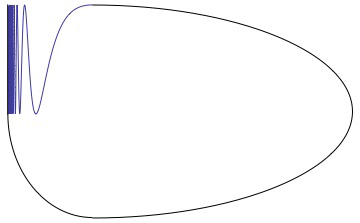
\includegraphics[scale = 0.8]{imagenes/Warsaw-circle.png}
  \caption{El círculo de Varsovia.}
  \label{circulovarsovia}
\end{figure}

Este espacio es conexo por caminos y simplemente conexo, de tal forma que la aplicación $ f:X\lra \{*\} $ induce isomorfismos en todos sus grupos de homotopía. Sin embargo, no se cumple en él el Teorema de Whitehead, puesto que no hay una equivalencia homotópica entre ambos: si la hubiera, pongamos $ H(x,0) = \id_{X} $ y $ H(x,1) = \{a\} $, entonces $ h_x(t) = H(x,t ) $ constituiría un camino uniendo $ x  $ y $ a  $. Por las propiedades del Círculo de Varsovia, sabemos que un tal camino no puede pasar por el tramo irregular, de tal forma que los puntos en la línea contigua a dicho tramo viajan a su imagen dando la vuelta por debajo y los puntos infinitamente próximos del tramo lo hacen superando las ondas, contra la continuidad de $ H  $. Sin embargo, las aplicaciones de $ \mathbb{S}^1 \lra U_n $ donde los $ U_n  $ son entornos de $ X  $ cada vez más cercanos sí se hacen cargo de su similitud con la circunferencia, y de hecho el grupo de dichos lazos es $ \Z  $, como lo es el grupo fundamental de la circunferencia.

Volvemos a la descripción de la forma de Borsuk. Borsuk considera espacios métricos compactos $ X, Y  $ inmersos en el cubo de Hilbert $ Q  $, y estudia sucesiones de aplicaciones entre sus entornos que llama \textbf{sucesiones fundamentales}, $ f_n:Q\lra Q  $ tales que
\begin{itemize}
  \item[] para todo entorno $ V$ de $Y  $ existe un entorno $ U  $ de $ X  $ (todos ellos en $ Q  $) que cumple $ f_n(U)\subc V  $ y $ \rest{f_n}{U} \simeq \rest{f_{n+1}  }{U }$ para casi todo $n$.
\end{itemize}
Dos sucesiones $ \underbar{f}, \underbar{g} $ son homótopas si todo entorno $ V  $ de $ Y  $ admite un entorno $ U  $ de $ X  $ tal que $ \rest{f_n}{U}\simeq \rest{g_n}{U} $ para casi todo $ n $. Esto define una relación de equivalencia entre sucesiones  que las divide en \textbf{clases fundamentales}. Podemos comprobar que la composición de clases componiendo sus representantes es una operación bien definida \cite[p. 232]{Borsuk_1968} y que la sucesión $ (\id_X ) $  es fundamental. Obtenemos así una categoría $ \Sh_B $ cuyos objetos son los compactos en $ Q $ y sus morfismos las clases fundamentales. Tal y como hacíamos en homotopía, diremos que dos espacios $ X$ e $Y $ tienen la misma \textbf{forma} si existen clases fundamentales $ [\underbar{f }]:X\lra Y  $, $ [\underbar{g}]:Y\lra X  $ tales que $ [\underbar{f}][\underbar{g}]  = [\id_{Y }] $ y $ [\underbar{g}][\underbar{f}]  = [\id_X ] $.     

Siguiendo a Christie, Borsuk presenta otro acercamiento a la forma a través de lo que denomina \textbf{aplicaciones aproximativas}: dados dos compactos $ X,Y\subc Q  $, son sucesiones de aplicaciones $ f_n: X\lra Q  $ tales que 
\begin{itemize}
  \item[] para todo $ V  $ entorno de $ Y  $ se tiene $ f_n\simeq f_{n+1}  $ en $V$ para casi todo $ n $.
\end{itemize}
Entre aplicaciones aproximativas también podemos definir una noción de homotopía, y diremos que $ (\vf_n) $ y $ (\psi_n) $ son homótopas si para todo entorno $ V  $ de $ Y  $ tenemos $ \vf_n\simeq \psi_n  $ en $ V  $ para casi todo $ n  $. De nuevo, esto define una relación de equivalencia a cuyas clases llamaremos \textbf{clases aproximativas}. Observamos que, aunque no podemos componer clases aproximativas porque los dominios no coinciden, sí podemos definir la composición de clases fundamentales con clases aproximativas componiendo representantes. Si asociáramos a cada clase aproximativa una fundamental, podríamos definir una categoría mediante esta operación. 

\begin{theorem}
  Existe tal asociaci'on y nos permite definir una categoría de compactos métricos que tiene por morfismos las clases aproximativas y es isomorfa a $ \Sh_B  $.
\end{theorem}
\begin{proof}
  Dada una aplicación aproximativa $ \vf = (\vf_n):X\lra Q  $, podemos extender cada aplicación $ \vf_n:X\lra Q  $ a una $ \Phi_n:Q\lra Q  $ porque el cubo de Hilbert es un AE. Todo entorno abierto $ V $ de $ Y  $ en $ Q  $ es abierto de un ANE, así que es ANE y, por tanto, ANR. Como $ \rest{\Phi_n}{X} \simeq \rest{\Phi_m}{X} $ en $ V  $, el Teorema \ref{extensionhomotopia} asegura que podemos extender esta homotopía de tal forma que $ (\Phi_n) $ sea una sucesión fundamental.

  Si tomamos otra aplicación aproximativa $ \psi = (\psi_n) $ homótopa a $ \vf  $, tenemos que las sucesiones fundamentales asociadas a cada una, $ \Psi  $ y $ \Phi  $ respectivamente, cumplen que para todo $ V $ entorno de $ Y  $ en $ Q  $,
  \begin{gather*}
    \rest{\Phi_n }{X } = \vf_n \simeq \psi_n  = \rest{\Psi_n }{X} \text{ en } V \text{ para casi todos } n,m .
  \end{gather*}
  De nuevo por el Teorema \ref{extensionhomotopia} podemos extender esta homotopía y, por tanto, la correspondencia establecida respeta las clases aproximativas. Esto significa que la composición de clases aproximativas $ [\psi]\circ [\vf ] $ está bien definida como $ [\Psi]\circ [ \vf ] $. Llamaremos a esta correspondencia $ F  $. Observamos que 
  \begin{gather*}
    F([\psi]\circ [\vf]) = F([\Psi \circ \vf])  \quad  \& \quad F([\psi])\circ F([\vf]) = [\Psi]\circ [\Phi ] = [\Psi \circ \Phi ]. 
  \end{gather*}
  Si tenemos un representante $ \Gamma  $ de $ F([\Psi \circ \vf]) $, es claro que para todo $ V  $ entorno de $ Y  $ en $ Q  $,
  \begin{gather*}
    \rest{\Gamma_n }{X} \simeq \Psi_n \circ \vf_n  = \rest{\Psi_n\circ \Phi _n}{X} \text{ en } V \text{ para casi todos } n,m,
  \end{gather*}
  de donde $ F  $ es un funtor por el argumento anterior. 

  La restricción a $ X  $ de una sucesíon fundamental $ \underbar{f} = (f_n):Q\lra Q  $ es una clase aproximativa por definición y, si dos sucesiones son homótopas, dichas clases lo son también. Además, la restricción conmuta con la composición y, por ende, esta asociación trivial es el funtor inverso de $ F  $. Esto implica que $ F  $ es un isomorfismo de categorías, como queríamos demostrar.
\end{proof}

Será útil más adelante tener en cuenta esta correspondencia entre aplicaciones aproximativas y sucesiones fundamentales. Mediante la noción de clase aproximativa se definen operaciones de producto e inversión y se da estructura de grupo a las clases aproximativas de $ \mathbb{S}^n\lra Y  $, lo que se llama el $ n $\textbf{-ésimo grupo de homotopía fundamental} de $ Y  $. De hecho, toda clase fundamental entre dos espacios induce de manera funtorial un homomorfismo entre sus grupos fundamentales\footnote{No confundir con el grupo fundamental de teoría de homotopía clásica.} y aunando ambas afirmaciones se obtiene un funtor $ \Sh_B \lra \text{Ab} $ para $ n>1  $ y en Grp para $ n=1 $.

Como afirmamos al principio, toda esta teoría se puede ver como una extensión interesada de la teoría de homotopía, puesto que sobre los espacios con buenas propiedades locales como los ANR's, coinciden. Esto es consecuencia de los siguientes hechos:
\begin{enumerate}
  \item Toda aplicación $ f:X\lra Y  $ se puede extender a una $ \hat{f}:Q\lra Q  $ por ser $ Q  $ un AE y $ X  $ cerrado en $ Q  $. Así, podemos formar una sucesión fundamental $ (f_n )_n  $ con $ f_n =  \hat{f} $.
  \item  \label{punto2} Si dos aplicaciones son débilmente homótopas, es decir, homótopas en cada entorno $ V  $ de $ Y  $ en $ Q  $, sus sucesiones fundamentales inducidas son homótopas. 
  \item La clase fundamental $ [\hat{f}] $ no depende de la extensión escogida.
  \item Si $ Y  $ es un ANR, toda clase fundamental $ [\underbar{f}]:X\lra Y  $ viene inducida por una aplicación $ f:X\lra Y  $.
  \item Si dos aplicaciones $ f,g:X\lra Y  $ generan la misma clase fundamental, entonces son débilmente homótopas.\label{punto5}
  \item Si dos aplicaciones entre ANR's son débilmente homotópas, entonces son homótopas. \label{punto6}
  \item Si dos ANR $ X  $ e $ Y  $ tienen la misma forma, entonces tienen el mismo tipo de homotopía. \label{punto7}
  \begin{proof}[Demostraci'on del Punto \ref{punto7}]
    Sean $ [\underbar{f}] $ y $ [\underbar{g}] $ las clases que nos dan la equivalencia de forma. Por ser ambos espacios ANR's, ambos morfismos vienen inducidos por aplicaciones continuas $ f:X\lra Y  $, $ g:Y\lra X  $. Como $ [g][f] = [\id_X ] $ y $ [f][g] = [\id_Y] $, son débilmente homótopas por el punto \ref{punto5}, y por el punto \ref{punto6} son homótopas.
  \end{proof}
\end{enumerate}
Como corolario de este desarrollo también podemos deducir que si dos espacios tienen el mismo tipo de homotopía, la equivalencia homotópica induce una equivalencia fundamental por el punto \ref{punto2} y tienen la misma forma. 

Después de la publicación del artículo de Borsuk, diversos autores intentaron generalizar la teoría más allá de los compactos métricos mediante nuevas aproximaciones. En 1970, S. Marde\v si\'c y J. Segal definieron la forma en espacios Hausdorff compactos \cite{Mardešić1970,Mardešić1971}, iniciando el acercamiento por sistemas inversos a la forma y poniendo la base para la generalización categórica del concepto, que vendría de la mano de Morita para espacios topológicos en general \cite{Morita1975}. Mientras tanto, Fox \cite{Fox1972} y  Borsuk \cite{borsuk1975} la generalizarían por distintas vías a espacios métricos generales. En Espa\~na, J. M. Sanjurjo dio una nueva descripción de la categoría forma basada en las aplicaciones multivaluadas \cite{sanjurjo_1990,sanjurjo_1992} que más tarde revisarían M. A. Morón y A. González \cite{ALONSOMORON2008972}.

Más progresos de la teoría siguieron llegando, consiguiendo probar teoremas análogos a los de Whitehead, Hurewicz \cite{Morita1975} y Smale \cite{dydak1978whitehead} sin las condiciones locales que aparecían como necesarias en la teoría de homotopía. Otra fuente de aplicaciones de la teoría de la forma serían los sorprendentes teoremas sobre complementos demostrados por Chapman \cite{chapman1972some,chapman1972shapes}, quien consiguió caracterizar la forma de un compacto métrico mediante el tipo topológico de su complementario en $ Q  $. 




\section{La forma mediante ANR-sistemas}\label{seccionanr}
En esta sección vamos a generalizar la teoría de la forma a compactos Hausdorff basándonos en el artículo \textit{Shape of compacta and ANR-systems} de S. Mard\v esi\'c y J. Segal \cite{Mardešić1971}. Esta descripción fue rápidamente generalizada a un nivel más abstracto que visitaremos en el Cap'itulo \ref{formacategorica}. La filosofía consistirá en asociar a cada espacio un sistema de espacios ANR y estudiar los morfismos entre estos sistemas, emulando lo que hacíamos mediante los entornos y las sucesiones fundamentales.

En lo que sigue, cuando hablemos de un ANR nos referiremos a un compacto ANR para la categoría de espacios métricos; cuando hablemos de un espacio $ X  $, será de la categoría Cpt de espacios compactos Hausdorff. 

\begin{definition}
    Diremos que un conjunto parcialmente ordenado $\Lambda $ es \textbf{dirigido} si, para todos $\lam_1,\lam_2\in \Lambda $, existe un $\lam\in \Lambda $ mayor que ambos, $\lam_1,\lam_2\leq \lam $. Diremos que es \textbf{cofinito} si el conjunto de predecesores de todo 'indice es finito. Un subconjunto $\Lambda'\subc \Lambda $ es \textbf{cofinal} si, para todo $\lam\in \Lambda $, existe $\lam'\in \Lambda ' $ tal que $\lam\leq \lam'$.
\end{definition}


\begin{definition}
  Sea $ \ccal  $ una categoría. Un \textbf{sistema inverso} $ \mathbf{X } $ en $ \ccal  $ está formado por un conjunto dirigido de índices $ \Lambda  $, un objeto $ X_\lambda  $ para cada $ \lambda \in \Lambda  $ y un \textbf{morfismo de paso} $ p_{\lam \lam' } : X_{\lam'} \lra X_\lam $ para cada par $ \lam\leq \lam'  $. Estos morfismos han de cumplir $ p_{\lam \lam }  = \id_{X_\lam } $ y que si tenemos $ \lam\leq \lam' \leq \lam''  $ entonces $ p_{\lam \lam'}p_{\lam'\lam ''} = p_{\lam \lam' } $. Si $ \Lambda  = \N  $, diremos que $ \mathbf{X } $ es una sucesión inversa.
\end{definition}

Diremos que un sistema inverso es un \textbf{ANR-sistema}\footnote{La traducci'on cl'asica al espa\~nol de este concepto es <<sistema de ANR's>>. En este texto preferimos <<ANR-sistema>> porque acorta la escritura y es m'as conveniente.} si el conjunto dirigido es cofinito, cada $ X_\lam  $ es un ANR y los morfismos de paso son funciones continuas. Dado un ANR $ X  $, podemos construir un ANR-sistema trivial asociado haciendo $ X_\lam = X  $ y $ p_{\lambda\lambda'} = \id_X  $. Un \textbf{morfismo de ANR-sistemas} o \textbf{ANR-morfismo} $ \mathbf{f}:\mathbf{X} = (X_\lam,p_{\lam\lam'},\Lambda)\lra \mathbf{Y} = (Y_\mu,q_{\mu\mu'},M )  $ consiste en una función creciente $ \vf:M \lra \Lambda  $ y aplicaciones $ f_\mu :X_{\vf(\mu)}\lra Y_\mu  $ tales que para todo $ \mu $, si $ \mu\leq \mu'  $, el siguiente diagrama conmuta en homotopía\footnote{A partir de aquí, cada vez que nos refiramos a la conmutatividad de un diagrama, será en homotopía a no ser que se especifique lo contrario.}:
\begin{center}
  \begin{tikzcd}
    X_{\vf(\mu)}\arrow{d}{f_\mu} & X_{\vf(\mu')} \arrow{d}{f_{\mu'}}\arrow{l} \\ 
    Y_\mu & Y_{\mu'} \arrow{l}
  \end{tikzcd}.
\end{center}
 Si cambiamos los sistemas por Cpt-sistemas, obtenemos un \textbf{Cpt-morfismo}. Denotaremos los morfismos desde un sistema trivial $(X,\id_X) $ como $\mathbf{f}:X\lra \mathbf{Y}$. El morfismo identidad es $ \mathbf{\id_\mathbf{X}} = (\id_{X_\lam},\id_\Lambda) $. La composición de dos morfismos $ (f_\mu, \vf ) $ y $ (g_\alf, \psi ) $ se define como el morfismo $ (g_\alf\circ f_{\psi(\alf )}, \vf\circ \psi ) $, y está bien definida por la conmutatividad de
\begin{center}
  \begin{tikzcd}
    X_{\vf\psi(\alf')} \arrow{d} \arrow{r}{f_{\psi(\alf')}} & Y_{\psi(\alf')} \arrow{r}{g_{\alf'}} \arrow{d} & Z_{\alf'} \arrow{d} \\ 
    X_{\vf\psi(\alf)} \arrow{r}{f_{\psi(\alf)}} & Y_{\psi(\alf)} \arrow{r}{g_{\alf}} & Z_\alf 
  \end{tikzcd}.
\end{center}

Diremos que dos morfismos de ANR-sistemas $ \mathbf{f},\mathbf{g}:\mathbf{X}\lra \mathbf{Y} $ son homótopos, $ \mathbf{f}\simeq \mathbf{g} $, si para todo $ \mu\in M  $ existe un índice $ \lam\geq \vf(\mu),\psi(\mu ) $ tal que el siguiente  diagrama conmuta:
\begin{center}
  \begin{tikzcd}
    X_{\vf(\mu)}\arrow[swap]{dr}{f_\mu} & X_{\lambda} \arrow[r] \arrow[l] & X_{\psi(\mu)} \arrow{dl}{g_\mu} \\ & Y_\mu &
  \end{tikzcd}.
\end{center}
Es rutinario comprobar que esta relación es de equivalencia por la conmutatividad del diagrama 
\begin{center}
  \begin{tikzcd}
    & & X_{\lam''}\arrow{dr}\arrow{dl} & & \\ 
    X_{\vf(\mu)} \arrow{drr}{f_\mu} & X_\lam \arrow{r}\arrow{l} & X_{\psi(\mu)} \arrow{d}{g_\mu} & X_{\lam'}\arrow{r} \arrow{l} & X_{\chi(\mu)} \arrow{dll}{h_\mu}\\ 
    & &Y_\mu & & 
  \end{tikzcd}
\end{center}
tomando $ \lam'' \geq \lam,\lam'  $. De hecho, esta relación de equivalencia respeta la composición de morfismos: si tenemos $ \mathbf{f},\mathbf{f}':\mathbf{X}\lra \mathbf{Y} $ y $ \mathbf{g},\mathbf{g}':\mathbf{Y}\lra \mathbf{Z } $ homótopos dos a dos, 
\begin{enumerate}
  \item primero, probamos que $ \mathbf{g}\mathbf{f}\simeq \mathbf{g}'\mathbf{f} $: existe un $ \mu\geq \psi(\alf),\psi'(\alf) $ tal que el siguiente diagrama conmuta:
  \begin{center}
    \begin{tikzcd}
      X_{\vf\psi(\alf)} \arrow{d}{f_{\psi(\alf)}} & X_{\vf(\mu )} \arrow{r} \arrow{d}{f_\mu} \arrow{l} & X_{\vf\psi'(\alf)} \arrow{d}{f_{\psi'(\alf)}} \\ 
      Y_{\psi(\alf)} \arrow{dr}{g_\alf} & Y_\mu \arrow{r} \arrow{l}  & Y_{\psi'(\alf)} \arrow{dl}{g_\alf} \\ 
      & Z_\alf &
    \end{tikzcd};
  \end{center}
  \item segundo, observamos que $ \mathbf{g}\mathbf{f}\simeq \mathbf{g}\mathbf{f}'  $ porque existe $ \lam\geq \vf\psi(\alf),\vf'\psi(\alf) $ que hace conmutativo
  \begin{center}
    \begin{tikzcd}
      X_{\vf\psi(\alf)} \arrow{dr}{f_{\psi(\alf)}} & X_\lam \arrow{r} \arrow{l} & X_{\vf'\psi(\alf)} \arrow{dl}{f_{\psi(\alf)}} \\ & Y_{\psi(\alf)} \arrow{d}{g_\alf} & \\ & Z_\alf & 
    \end{tikzcd}
  \end{center}.
\end{enumerate}
Diremos que un ANR-morfismo $ \mathbf{f} $ es una \textbf{equivalencia homotópica} si existe $ \mathbf{g} $ tal que $ \mathbf{g}\mathbf{f}\simeq \id_X  $ y $ \mathbf{f}\mathbf{g}\simeq \id_Y  $. Diremos que dos sistemas tienen el mismo \textbf{tipo de homotopía} si existe una equivalencia homotópica entre ellos. Gracias a lo que acabamos de ver, sabemos que esta relación es de equivalencia y divide la categoría de ANR-sistemas y ANR-morfismos en clases de equivalencia. 

\begin{definition}
  Un \textbf{límite inverso} de un Cpt-sistema $ \mathbf{X} $ son un $ X \in \text{Cpt} $ y un Cpt-morfismo $ \mathbf{p}:X\lra \mathbf{X} $ con la propiedad universal siguiente: para todo Cpt-morfismo  $ \mathbf{g}:Y \lra \mathbf{X} $ con $ Y\in \text{Cpt} $, existe una aplicación continua $ g:Y\lra X  $ tal que $ \mathbf{p}g = \mathbf{g} $.
\end{definition}
\begin{observation}
  Para cualquier otro límite inverso $ \mathbf{p}':X'\lra \mathbf{X} $, la aplicación  $ g:X\lra X'  $ es un homeomorfismo, es decir, el límite inverso es único. Escribiremos $ X = \displaystyle\lim_{\longleftarrow}\mathbf{X}  $ y diremos en tal caso que $ \mathbf{X} $ está \textbf{asociado} con el espacio $ X  $.
\end{observation}

De la misma forma, si tenemos sistemas $ \mathbf{X} $, $ \mathbf{Y} $ asociados a espacios $ X $, $ Y$, diremos que los morfismos $ \mathbf{f}:\mathbf{X}\lra \mathbf{Y} $ y $ f:X\lra Y  $ están \textbf{asociados} si el siguiente diagrama conmuta:
\begin{center}
  \begin{tikzcd}
    X_{\vf(\mu)}\arrow{d}{f_\mu} & X \arrow{l}{p_{\vf(\mu)}} \arrow{d}{f} \\ 
    Y_\mu & Y \arrow{l}{q_\mu}
  \end{tikzcd}.
\end{center}


\begin{theorem}\label{teoremavietoris}
  Todo espacio compacto Hausdorff admite un \emph{ANR}-sistema asociado.
\end{theorem}
\begin{proof}
  Si el cardinal de $ X  $ es finito, entonces $ X  $ ya es un poliedro y el sistema trivial es suficiente. Por el Teorema de Inmersi'on de Tykhonov \cite[17.11]{willard1970general}, $ X  $ se puede considerar como un subconjunto del producto infinito de intervalos unidad $ I^\Omega  = \prod_{\omega\in \Omega}I_\omega  $, donde el cardinal de $ \Omega  $ es igual al peso de $ X  $, es decir, el menor cardinal de sus bases de abiertos. Vamos a ver que podemos construir un sistema inverso con l'imite inverso $ I^{\omeg } $ de tal forma que al restringirnos a $ X  $ obtengamos el deseado.
  
  Consideramos $ \Lambda = F(\omeg ) $ el conjunto de subconjuntos finitos no vac'ios de $ \omeg $, ordenado por la inclusi'on. Para $ \lam = \{\omega_1,...,\omega_n\} $, definimos $ I^\lam = I_{\omega_1}\times\cdots \times I_{\omega_n } $. Si $ \lam\leq \lam'  $, la proyecci'on natural $ p_{\lam\lam'}:I^{\lam'}\lra I^\lam  $ completa un sistema inverso $ (I^\lam,p_{\lam\lam'},\Lambda ) $ cuyo l'imite inverso es $ I^\omeg $ mediante la proyecci'on natural $ p_\lam:I^\omeg\lra I^\lam  $.

  Para cada $ \lam\in \Lambda  $, denotamos por $  \abs{\lam} $ su cardinal. Construimos una sucesi'on de abiertos $ U^\lam_n\subc I^\lam  $ tales que:
  \begin{enumerate}
    \item $ p_\lam (X) = \bigcap_n U_n ^\lam  $,
    \item $ U^\lam_1 \supset \ol{U^\lam_2}\supset U^\lam_2 \supset U_{3}^\lam \supset U_4^\lam \supset \cdots  $,
    \item $ p_{\lam\lam'}(U^{\lam'}_1)\subseteq U^\lam_{\abs{\lam'}-r\abs{\lam}+1} $, para todo $ \lam\leq \lam'  $.
  \end{enumerate}
  Por inducci'on en $ \abs{\lam} $, si $ \abs{\lam} = 1 $, podemos escoger los $ U_n^\lam  $ libremente para que satisfagan las dos primeras condiciones. Si ahora tomamos $ \lam'$ y  lo suponemos probado para todo $ \lam  $ con cardinal $  \abs{\lam}<\abs{\lam' } $, 
  \begin{gather*}
    p_{\lam\lam'}(p_{\lam'}(X)) = p_\lam(X) \subc U_{\lam,\abs{\lam'}-\abs{\lam}+1}.
  \end{gather*}
  Como solo hay una cantidad finita de estos $ \lam <\lam'   $, podemos encontrar un entorno abierto $ U_1^{\lam' } $ de $ p_{\lam'}(X ) $ que cumpla la tercera propiedad. Despu'es, definimos el resto de sucesi'on de entornos para que se cumplan las dem'as propiedades.

  Claramente, para todo $ \lam\in \Lambda  $ podemos encontrar un poliedro $ X_\lam\subc I^\lam  $ tal que 
  \begin{gather*}
    \ol{U_2^\lam }\subc X_\lam \subc U_1^\lam.
  \end{gather*}
  Combinando esto con lo anterior, para todo $ \lam<\lam'  $ se tiene 
  \begin{gather*}
    p_{\lam\lam'}(X_{\lam'}) \subc p_{\lam\lam'}(U_{1}^{\lam'}) \subc U^\lam_{\abs{\lam'}-\abs{\lam}+1} \subc U_1^\lam \subc X_\lam,
  \end{gather*}
  y, por ende, $ (X_\lam,p_{\lam\lam'},\Lambda ) $ es un sistema inverso de poliedros (que son ANR's por el Teorema \ref{complejoanr}). Su l'imite inverso $ \xfrak  $ cumple que, para todos $ y\in \xfrak  $ y $ \lam\leq\lam'$,
  \begin{gather*}
    p_\lam\py = p_{\lambda\lambda'}p_{\lam'}\py \in p_{\lambda\lambda'}(X_{\lam'}) \subc U^\lam_{\abs{\lam'}-\abs{\lam}+1}.
  \end{gather*}
  Como $ \lam'  $ puede ser de cardinal arbitrariamente grande, esto implica que para todo $ \lam\in \Lambda  $ 
  \begin{gather*}
    p_\lam(y)\in \bigcap_n U^\lam_n = p_\lam(X)
  \end{gather*}
  y por tanto $ y\in X  $. Rec'iprocamente, $ p_\lam (X)\subc U_2^\lam \subc X_\lam  $, de donde se colige que $ X\subc \xfrak  $, como quer'iamos demostrar.
\end{proof}

\begin{observation}
  Todo espacio compacto m'etrico $ X  $ tiene una base numerable. Esto implica que el peso de $ X  $ es menor o igual que $ \aleph_0  $, y la demostraci'on anterior prueba que existe una ANR-sucesi'on de poliedros asociada a $ X  $.
\end{observation}

Visto esto, podemos asociar a cada $ X  $ una clase de homotopía de ANR-sistemas, y esto es lo que llamaremos la \textbf{forma} de $ X  $, y denotaremos por $ \Sh(X)  $. Sin embargo, no hemos demostrado que esta clase sea única, es decir, que dos sistemas asociados con el mismo espacio sean siempre homótopos. Esto es consecuencia de los siguientes hechos:
\begin{enumerate}
  \item \label{teorema8} Si tenemos morfismos $ \mathbf{f}:\mathbf{X}\lra \mathbf{Y} $, $ \mathbf{g}:\mathbf{Y}\lra \mathbf{Z} $ asociados con morfismos $ f:X\lra Y  $, $ g:Y\lra Z  $, entonces $ \mathbf{g}\mathbf{f}  $ está asociado con $ gf  $; además, $ \mathbf{\id_X}:\mathbf{X}\lra \mathbf{X} $ está asociada con la identidad $ \id_X:X\lra X  $.
  \item Si $ \mathbf{f} $ está asociado con $ f  $ y tenemos otro morfismo $ \mathbf{g}\simeq \mathbf{f} $, entonces $ \mathbf{g} $ también está asociado con $ f  $.
  \item \label{teorema10} Toda aplicación $ f:X\lra Y  $ tiene un ANR-morfismo $ \mathbf{f}:\mathbf{X}\lra \mathbf{Y} $ asociado.
  \item \label{homotopia} Si tenemos $ \mathbf{f} $, $ \mathbf{g} $ asociados con $ f  $, $ g  $, entonces $ f\simeq g  $ implica $ \mathbf{f}\simeq \mathbf{g} $.
  \item \label{ultimopunto} Si $ X  $ e $ Y  $ tienen el mismo tipo de homotopía, cualesquiera sistemas asociados $ \mathbf{X} $ e $ \mathbf{Y} $ también lo tienen, así que tienen la misma forma.
  \begin{proof}[Demostraci'on del Punto \ref{ultimopunto}]
    Sabemos que hay aplicaciones $ f:X\lra Y  $, $ g:Y\lra X  $ tales que $ gf\simeq \id_X  $ y $ fg\simeq \id_Y  $. Por el punto \ref{teorema10}, existen ANR-morfismos $ \mathbf{f}:\mathbf{X}\lra \mathbf{Y} $ y $ \mathbf{g}:\mathbf{Y}\lra \mathbf{X}$ asociados, y por el punto \ref{teorema8}, $ \mathbf{g}\mathbf{f} $ y $ \mathbf{f}\mathbf{g} $ están asociados con $ gf  $ y $ fg  $. Es más, por el punto \ref{homotopia}, $ \mathbf{g}\mathbf{f}\simeq \mathbf{\id_{\mathbf{X}}} $ y $ \mathbf{f}\mathbf{g}\simeq \mathbf{\id_{\mathbf{Y}}} $, de donde tienen la misma forma.
  \end{proof}
\end{enumerate}

Al igual que en el caso de Borsuk, la forma es un invariante por homotopía, y si nos ponemos en el caso de espacios ANR, coinciden: si $ X  $ e $ Y  $ son ANR's, sabemos que los sistemas triviales $ (X,\id_X) $ y $ (Y,\id_Y ) $ son ANR-sistemas asociados; que tengan la misma homotopía implica que existe una equivalencia homotópica de sistemas dada por $ \mathbf{f}:(X)\lra (Y) $ y $ \mathbf{g}:(Y)\lra (X) $, pero en este caso ambos morfismos se reducen a morfismos $ f:X\lra Y  $ y $ g:Y\lra X  $ que nos dan una equivalencia homotópica.

\begin{theorem}
  La categoría de compactos métricos y ANR-morfismos es isomorfa a $ \Sh_B  $.
\end{theorem}
\begin{proof}
  Todo compacto métrico $ X  $ admite un ANR-sistema sencillo asociado, consistente en tomar entornos abiertos cada vez más peque\~nos en $ Q  $ ordenados por la inclusión, $ X_n := X_{\frac{1}{n}} = \{x\in Q\mid \dd(x,X_n)<\frac{1}{n}\} $. El límite inverso será $ \bigcap_n X_n = X  $. Trabajaremos con estos sistemas durante toda la demostración. 

  Para definir un funtor entre las categorías, tomamos primero una sucesión fundamental $ \underline{\vf}:X\lra Y  $. Dado $ n\in \N $, $ Y_n  $ es un entorno de $ Y  $, de donde existen un índice $ n_0 $ y un entorno $ U_n  $ tales que $ \vf_m (U_n)\subc Y_n  $ y $ \rest{\vf_m}{U_n }\simeq \rest{\vf_{m+1}}{U_n } $ en $ Y_n  $ para todo $ m\geq n_0  $. Podemos tomar $ n_1  $ tal que, si $ k\geq n_1  $, $ X_k\subc U_n  $. Escogiendo una función creciente $ f:\N \lra \N  $ que cumpla $ f(n)\geq n_0,n_1 $, tenemos que $ X_{f(n)}\subc U_n  $, y por ende para todo $m\geq f(n)  $, $ \rest{\vf_m }{X_{f(n)}}\simeq \rest{\vf_{m+1}}{X_{f(n)}} $ en $ Y_n  $. Podemos definir $ f_n = \rest{\vf_{f(n)}}{X_{f(n)}} $, que es un ANR-morfismo porque, dados $ n\leq m  $, 
  \begin{gather*}
    f_n = \rest{\vf_{f(n)}}{X_{f(n)}} \simeq \rest{\vf_{f(m)} }{X_{f(n )}} \text{ en } Y_n, 
  \end{gather*}
  y esto implica que, restringiendo a $ X_{f(m)} $, 
  \begin{gather*}
    \rest{f_n }{X_{f(m)}} \simeq \rest{\vf_{f(m)} }{X_{f(m )}}  = f_m \text{ en } Y_n.
  \end{gather*} 
  Hemos deducido así que $ f_n i_{f(n)f(m)} \simeq j_{nm} f_{m} $, como queríamos demostrar.

  Esta asociación no es sobreyectiva sobre el conjunto de ANR-morfismos, pero sí lo es sobre el conjunto de ANR-morfismos regulares: aquellos que tienen función de índices $ \vf  $ estrictamente creciente. Esto es suficiente para establecer una biyección entre clases de ANR-morfismos y clases fundamentales, puesto que toda clase de ANR-morfismos tiene un representante regular. Solo queda demostrar que hemos definido un funtor: sean $ \underline{\vf}:X\lra Y  $ y $ \underline{\psi }:Y\lra Z  $ sucesiones fundamentales asociadas con $ \mathbf{f} = (f_n,f):\mathbf{X}\lra \mathbf{Y} $ y $ \mathbf{g}=(g_n,g):\mathbf{Y}\lra \mathbf{Z} $ respectivamente. Queremos ver que la clase asociada a $ [\underline{\psi }][\underline{\vf }] $ es $ [\mathbf{g}][\mathbf{f}] $. 
  
  Por definición, si $ m\geq fg(n) $, entonces 
  \begin{gather*}
    \rest{\vf_m }{X_{fg(n)}} \simeq \rest{\vf_{fg(n)}}{X_{fg(n )}}  = f_{g(n)} \text{ en } Y_{g(n )}.
  \end{gather*}
  De igual modo, si $ m\geq g(n)  $,
  \begin{gather*}
    \rest{\psi_m}{Y_{g(n )}} \simeq \rest{\psi_{g(n) }}{Y_{g(n)}}  =g_n \text{ en } Z_n .
  \end{gather*}
  Si escogemos una función $ h:\N \lra \N  $ creciente tal que $ h(n)\geq fg(n),g(n) $, entonces 
  \begin{gather*}
    h_n = \rest{\psi_{h(n)}\vf_{h(n)}}{X_{h(n)}} \simeq g_n f_{g(n)} \text{ en } Z_n.
  \end{gather*}
  Es claro que $ \mathbf{h}= (h_n, h)$ está asociado a $\underline{\psi}\underline{\vf } $ y, además, $ \mathbf{h }\simeq \mathbf{g}\mathbf{f} $, por lo que ambas clases coinciden, y esto concluye la demostración. Los detalles sobre esta demostración se pueden consultar en el artículo \textit{Equivalence of the Borsuk and the ANR-system approach to shapes} de Marde\v si\'c y Segal \cite{mardevsic1971equivalence}.
\end{proof}


\section{La Forma mediante aplicaciones multivaluadas}
Como comentábamos en la primera sección, J. M. Sanjurjo  \cite{sanjurjo_1990,sanjurjo_1992} introdujo una nueva descripción de la forma en la categoría de compactos métricos basándose en las aplicaciones multivaluadas y descripción de la forma de Christie mediante las aplicaciones aproximativas \cite{christie1944net}. Esta descripción de la forma es intrínseca en el sentido de que no necesita de expansiones y espacios distintos del propio compacto métrico para describir los morfismos y definir la forma. A lo largo de la sección, $ X $ e $ Y  $ denotarán compactos métricos si no indicamos lo contrario.

Una \textbf{función multivaluada} $ F:X\lra Y  $ es una correspondencia que a cada $ x\in X  $ le asigna un conjunto cerrado $ F(x)\subc Y  $. Diremos que es \textbf{semicontinua superiormente} si para todo $ x\in X  $ y $ V \subc Y $ entorno de $ F(x) $ existe un entorno $ U\subc X  $ del punto tal que $ F(U) = \bigcup \{F(x')\mid x'\in U \} $ está contenido en $ V  $. El papel de las homotopías en la teoría clásica lo juegan ahora las $ \eps $-homotopías:
\begin{definition}
  Diremos que una función multivaluada es $ \eps  $-\textbf{peque\~ na} si \\ $ \diam(F(x))<\eps  $ para todo $ x\in X  $. 

  Dos aplicaciones $ \eps $-peque\~ nas son $ \eps  $\textbf{-multihom'otopas} si existe una aplicación multivaluada semicontinua superiormente  
  \begin{gather*}
    H:X\times I\lra Y 
  \end{gather*}
  $ \eps  $-peque\~ na que cumple $ H(x,0) = F\px  $ y $ H(x,1) = G\px  $. Lo denotaremos $ F\simeq_\eps G  $ y llamaremos a $ H  $ una $ \eps  $\textbf{-multihomotopía}.   
\end{definition}
Observamos que, si $ Y  $ es un compacto métrico, toda aplicación multivaluada es $ \eps  $-peque\~na para algún $ \eps>0  $. Ser aplicaciones $ \eps  $-multihomótopas define una relación de equivalencia. Ya podemos definir e análogo a una sucesión fundamental:
\begin{definition}
  Una \textbf{multirred} de $ X  $ en $ Y  $ es una sucesión de funciones multivaluadas $ F_n:X\lra Y  $ tal que para todo $ \eps>0  $ existe un $ n_0\in \N  $ tal que $ F_n \simeq_\eps F_{n+1} $ para todo $ n\geq n_0  $. Las representaremos en negrita como $ \mathbf{F}:X\lra Y  $.
\end{definition}
Dadas dos multirredes $ \mathbf{F},\mathbf{G}:X\lra Y  $, diremos que son homótopas si para todo $ \eps>0  $ se tiene $ F_n\simeq_\eps G_n  $ para casi todo $ n \in \N  $. En la demostración de la equivalencia de categorías nos serviremos de un tipo más de funciones:



Diremos que una aplicación aproximativa $ \vf  $ se obtiene de una multirred $ \mathbf{F} $ si para todo $ \eps>0  $ se tiene $ \dd(\vf_n,F_n)<\eps  $ para casi todo $ n $. Para asociar una aplicación aproximativa a una multirred, demostramos el siguiente lema:
\begin{lemma}[de Aproximación] \label{lemaaproximacion}
  Para toda aplicación multivaluada $ \eps  $-peque\~na $ F:Y\lra Q  $ con $ Y  $ compacto existe una aplicación $ f:Y\lra Q  $ tal que $ \dd(f,F)<\eps  $.
\end{lemma}
\begin{proof}
  Asumimos que $ Y  $ tiene más de un punto (de lo contrario, el resultado es trivial). Como $ F  $ es semicontinua superiormente, para todo $ y\in Y  $ existe un entorno $ V  $ tal que $ F(V)\subc B(F(y),r) $, donde $ r = \frac{\eps-\diam(F(y))}{3} $. Recopilando estos entornos y usando la compacidad de $ Y  $, existe un recubrimiento abierto finito $ \{Y_i\}_{i=1,..,n} $ de abiertos no vacíos, distintos entre sí y tales que $ \diam(F(Y_i)) < 2r+\diam(F(y)) < \eps  $. Para cada $ i=1,...,n  $, definimos la función 
  \begin{gather*}
    \lam_i(y) = \frac{\dd(y,Y\setminus Y_i)}{\sum_{j=1}^{n}\dd(y,Y\setminus Y_j )}.
  \end{gather*}
  Estas funciones son claramente continuas y $ \lam_i(y) \neq 0  $ si y solo si $ y\in Y_i  $. Para construir $ f:Y\lra Q  $, escogemos un punto $ x_i \in F(Y_i) $ para cada $ i  $ y los pegamos mediante las funciones $ \lam_i$:
  \begin{gather*}
    f\py = \sum_{i=1}^{n} \lam_i(y)x_i .
  \end{gather*}
  Esta función es continua por serlo las $ \lam_i  $ y se cumple que para todo $ y\in Y  $, si tomamos $ x\in F(y)  $, 
  \begin{gather*}
    \dd(x,f\py)\leq \norm{x-\sum_{i=1}^{n}\lam_i\py x_i}  = \norm{\sum_{i=1}^{n }\lam_i\py (x-x_i )}\leq \sum_{i=1}^{n } \lam_i\py \norm{x-x_i} < \\  \eps \sum_{i=1 }^{n }\lam_i\py  = \eps,
  \end{gather*}
  como queríamos demostrar. 
\end{proof}
Dadas una multirred $ \mathbf{F } = (F_n)_n$ y una sucesión decreciente que tiende a cero $ (\eps_n)_n  $, por el Lema de Aproximación \ref{lemaaproximacion}, para cada $ F_n:X\lra Y \subc Q $ existe una aplicación $ \vf_n:X\lra Q $ a distancia $ \dd(\vf_n,F_n)<\eps_n $. Nuestro objetivo es probar que es una aplicación aproximativa. Para todo entorno $ V  $ de $ Y  $ en $ Q  $, por ser $ Y  $ cerrado en $ Q  $, existe un $ n_0  $ tal que $ Y_{2\eps_{n_0}} = \{z\in V\mid \dd(z,Y)<2\eps_{n_0}\} $ está contenido en $ V  $. Tal vez aumentando $ n_0  $, podemos conseguir $ F_n \simeq_{\eps_{n_0}} F_{n+1}$ para $ n\geq n_0 $. Si llamamos $ H_{n_0}  $ a esta $ \eps_{n_0} $-multihomotopía, podemos usar de nuevo el Lema de Aproximación \ref{lemaaproximacion} para obtener una homotopía $ H  $ a distancia $ \dd(H_{\eps_{n_0}},H)<\eps_{n_0}  $. Denotamos $ f_n = H(x,0) $ y $ f_{n+1} = H(x,1) $ y observamos que
\begin{gather*}
  \dd(\vf_n,f_n)\leq \dd(\vf_n,F_n)+\dd(F_n,f_n)<2\eps_{n_0},
\end{gather*}
e igualmente para $ n+1$. Así pues, tenemos dos aplicaciones $ \vf_n,f_n:X\lra Y  $ a distancia menor que $ 2\eps_{n_0} $. Esto implica que la función 
\begin{gather*}
  \begin{matrix}
  G : \ &X\times I  &\longrightarrow &V  \\
  &(x,t) &\mapsto &t\vf_n\px +(1-t)f_n\px 
  \end{matrix}  
\end{gather*}
tiene su imagen contenida en $ Y_{2\eps_{n_0}}\subc V  $ y por tanto $ \vf_n\simeq f_n  $. Si repetimos el argumento para $ f_{n+1} $, conseguimos $ \vf_n \simeq f_n\simeq f_{n+1}\simeq \vf_{n+1} $, como queríamos demostrar.

Esta demostración prueba también que para cualquier otra elección $ \mathbf{G} \simeq \mathbf{F}$ que hubiéramos hecho, la aplicación aproximativa resultante sería homótopa a $ \vf  $, y por tanto una clase de homotopía de multirredes determina una única clase aproximativa. Vamos a probar que esta correspondencia es biyectiva:
\begin{theorem}
  La correspondencia $ \omega: [\mathbf{F }]\mapsto[ \vf]  $ entre multirredes y clases aproximativas descrita anteriormente es biyectiva.
\end{theorem}
\begin{proof}
  Primero, veamos la sobreyectividad. Sea $ [\vf]$ una clase aproximativa y $ (\eps_n)_n  $ una sucesión decreciente que tiende a cero. Para cada $ n\geq 1 $, si consideramos el entorno $ Y_{\eps_n } $ de $ Y  $, sabemos que existe un $ m_0\geq n$ tal que para todo $ m\geq m_0  $ se tiene $ \vf_m \simeq \vf_{m+1} $ en $ Y_{\eps_n } $. Si eliminamos los términos previos a  $ m_0 $ de la sucesión para cada $ n  $, obtenemos un nuevo representante de la misma clase aproximativa que cumple $ \vf_n\simeq \vf_{n+1}  $ en $ Y_{\eps_n } $ para todo $ n\geq 1 $. Denotamos a esta homotopía $ H_n  $, y definimos ahora 
  \begin{gather*}
    F_n (x) = \{y\in Y\mid \dd(y,\vf_n(x))\leq \eps_n/3 \}.
  \end{gather*}
  Para todo $ \eps>0  $, sea $ n_0 \in \N  $ tal que  $ \eps_{n_0}<\eps  $. Entonces, para todo $ n\geq n_0  $, la función multivaluada 
  \begin{gather*}
    \hat{H}_n(x,t)  = \{y\in Y\mid \dd(y,H_n(x,t))\leq \eps_n/3 \}
  \end{gather*}
  es semicontinua superiormente por ser $ H_n $ continua y es $ \eps_n  $-peque\~na. Además, cumple que $ \hat{H}_n(x,0) = F_n(x) $ y $ \hat{H}_n(x,1) = F_{n+1}(x) $, de donde ambas son $ \eps $-multihomótopas y $ \mathbf{F} = (F_n)_n  $ es una multirred. Llamemos $ [\psi ]= \omega([\mathbf{F }]) $. Para todo entorno $ V $ de $ Y  $ en $ Q  $, dado que para todo $ n\geq 1 $ 
  \begin{gather*}
    \dd(\vf_n,\psi_n)\leq \dd(\vf_n,F_n)+\dd(F_n,\psi_n) <\eps_n/3+\eps_n <2\eps_n,
  \end{gather*}
  podemos encontrar (por el desarrollo hecho en la definición de $ \omega  $) $ n_0 $ suficientemente grande tal que dos aplicaciones $ 2\eps_n $-cercanas sean homótopas para todo $ n\geq n_0 $. Esto prueba la sobreyectividad.


  Para la inyectividad, supongamos que $ [\vf]  = \omega([\mathbf{F}]) = \omega([\mathbf{G}])  = [\psi ]$. Para todo $ \eps>0  $, existe un $ n_0  $ tal que $ \eps_n<\eps/3  $ y  $ \vf_n \simeq \psi_n  $ en $ Y_{\eps}$ para $ n\geq n_0 $. Llamamos a esta homotopía $ H_n  $ y definimos $ \hat{H}_n(x,t) = \{y\in Y\mid \dd(y,H_n(x,t))\leq \eps/3 \}$. Esta es una aplicación multivaluada $ \eps  $-peque\~na y cumple $ F_n(x)\subc \hat{H}(x,0) $ y $ G_n(x)\subc \hat{H}(x,1) $, así que son $ \eps  $-multihomótopas, como queríamos demostrar.
\end{proof}

Para elevar el conjunto de multirredes a categoría, necesitamos una noción de composición. Sin embargo, la composición componente a componente no es necesariamente una multirred porque la composición de aplicaciones $ \eps  $-peque\~nas no tiene por qué serlo. Sanjurjo soluciona el problema definiendo la composición de clases de homotopía de multirredes $ \mathbf{F}:X\lra Y  $, $ \mathbf{G}:Y\lra Z  $ escogiendo una cierta sucesión $ (k_n)_n  $  y haciendo $ [\mathbf{G}]\circ [\mathbf{F}] = [(G_n \circ F_{k_n})_n] $. El modo de construir esta sucesión es el siguiente: se escoge una sucesión de reales decreciente que tiende a cero, $ (\eps_n)_n  $, para la cual $ G_m  $ es $ \eps_{n} $-multihomótopa a $ G_{n} $ para $ m\geq n  $ (se puede conseguir eliminando miembros de la sucesión sin modificar su clase de homotopía) y otra $ (\mu_n)_n  $ tal que $ \diam(G_n(K))<\eps_n  $ para todo $ K\subc Y  $ de $ \diam(K)<\mu_n  $\footnote{Esto es posible por la compacidad de $ X  $: dado $ x\in X  $, para todo $ \eps>0 $, por la semicontinuidad superior existe un $ \delta_x>0  $ tal que, si $ \dd(x,y)<\delta  $, entonces $ \dd(G_n(x),G_n(y))<\eps  $. La unión $ \bigcup_{x\in X}B(x,\delta_x) $ es un recubrimiento de $ X  $ y podemos encontrar un número $ \ro>0  $ de Lebesgue para el recubrimiento de tal forma que para todo $ \eps>0  $ y $ x,y\in X  $, si $ \dd(x,y)<\ro  $, entonces $ \dd(G_n(x),G_n(y))<\eps  $. Si tomamos $ \eps=\eps_n  $ y $ \mu_n = \ro/2 $, obtenemos la sucesión deseada.}.  Entonces $ (k_n)_n $ es una sucesión creciente de índices tal que $ F_k  $ es $ \mu_n  $-multihomótopa a $ F_{k_n} $ para todo $ k\geq k_n  $. Esta definición de composición nos lleva al teorema final 
\begin{theorem}[Sanjurjo]
  La categoría de compactos métricos y clases de homotopía de multirredes, que denotaremos \emph{HN}, es isomorfa a la categoría forma de compactos métricos.
\end{theorem}
\begin{proof}
  Veamos que la definición de composición asegura que hemos definido una multirred. Para todo $ \eps>0  $, tomamos $ n_0 $ tal que $ \eps_{n_0}<\eps $. Sabemos que $ G_n\simeq_{\eps_n}G_{n_0} $, y llamamos $ H_{n} $ a esta homotopía. Por el mismo razonamiento de antes, podemos escoger $ m_0\geq n_0  $ suficientemente grande de tal forma que, si $ \diam(K)<\mu_{m_0}  $ para $ K\subc Y\times I  $, entonces $ \diam(H_n(K))<\eps_{n_0} $. Para este índice, $ F_{k_{n}}\simeq_{\mu_0} F_{k_{m_0}} $ si $ n\geq m_0 $ por una $ \mu_{m_0} $-multihomotopía que denotamos $ L_{m_0} $. Si consideramos ahora $ H_{n}(L_{m_0}(x,t),t) $, esta es una aplicación multivaluada $ \eps_{n_0} $-peque\~na que nos da la homotopía $G_{n_0}F_{k_{m_0}}\simeq_{\eps_{n_0}}G_nF_{k_n} $. Por último, dado que $ F_{k_{n_0}}\simeq_{\mu_{n_0}} F_{k_{m_0}} $, podemos concluir que $ G_{n_0}F_{k_{n_0}}\simeq _{\eps_{n_0}} G_nF_{k_n} $ para todo $ n\geq n_0  $, como queríamos demostrar.

  Tenemos que demostrar ahora que la composición no depende de los representantes. Sean multirredes $ \mathbf{F},\mathbf{F'}:X\lra Y  $ y $ \mathbf{G},\mathbf{G'}:Y\lra Z $ con $ [\mathbf{F}] = [\mathbf{F'}] $ y $ [\mathbf{G}] = [\mathbf{G'}] $. Denotaremos $ (\eps'_n)_n  $, $ (\mu'_n)_n ,(k'_n)_n  $ a las sucesiones que intervienen en la definición de $ [\mathbf{G'}][\mathbf{F' }] $. Sea $ \eps>0 $ y consideremos $ n_0 $ tal que $ \eps_{n_0},\eps'_{n_0}<\eps  $, $ G_{n_0} \simeq_{\eps}G'_{n_0} $ y $ G_nF_{k_n}\simeq_\eps G_{n_0}F_{k_{n_0}} $ y $ G'_nF'_{k'_n}\simeq_\eps G'_{n_0}F'_{k'_{n_0}}  $ para todo $ n\geq n_0 $. Si tomamos $ m_0 \geq n_0 $ que garantice $ G_{n_0}F_{k_{m_0}}\simeq_\eps G'_{n_0}F_{k_{m_0}} $ como hicimos antes y también $ F_{k_{m_0}}\simeq_{\mu'_{n_0}} F'_{k'_{m_0}} $, entonces 
  \begin{gather*}
    G_{n_0}F_{k_{n_0}} \simeq_\eps G_{n_0}F_{k_{m_0}}\simeq_\eps G'_{n_0}F_{k_{m_0}} \simeq_\eps  G'_{n_0}F'_{k'_{m_0}} \simeq_\eps G'_{n_0}F'_{k'_{n_0}}.
  \end{gather*}

  Resta demostrar que la correspondencia $ \omega $ define un isomorfismo de categorías. Llamaremos $ \Omega :\text{HN}\lra \Sh_B $ al funtor $ \Omega(X) = X  $ y $ \Omega ([\mathbf{F}]) = \omega([\mathbf{F}]) $. Hemos de probar que $ \Omega([\mathbf{G}])\circ \Omega([\mathbf{F}]) = \Omega ([\mathbf{G}][\mathbf{F}]) $. Denotaremos $\Omega ([G_nF_{k_n}]) = [\vf] $, $ \Omega([\mathbf{F}]) = [\gamma  ] $, $ \Omega([\mathbf{G}]) = [\psi] $, y $ \Psi $ la extensión de $ \psi  $ tal que $ [\psi]\circ[\gamma] = [\Psi \circ \gamma ] $.
  
  Sea $ (\eps_n)_n  $ una sucesión decreciente que tiende a cero tal que 
  \begin{enumerate}
    \item $ \dd(\vf_n,G_nF_{k_n})<\eps_n  $,
    \item $ \dd(\psi_n,F_{k_n})<\eps_n  $, 
    \item $ \dd(\gamma_n,G_n)<\eps_n  $.
  \end{enumerate}
  Queremos probar que para todo $ V   $ entorno abierto de $ Y  $ en $ Q  $, $ \vf_n\simeq \Psi_n\circ \gamma_n  $ en $ V  $. Sea $ \ro>0  $ tal que todas dos aplicaciones $ \ro $-cercanas en $ V  $ son homótopas. Sabemos que si $ y\in F_{k_n}(x) $,
  \begin{gather*}
    \dd(\vf_n(x),\Psi_n \circ \gamma_n\px)\leq \dd(\vf_n(x),G_nF_{k_n}(x)) + \dd (G_nF_{k_n}\px,\Psi_n(F_{k_n}\px))+\\ 
    \dd(\Psi_n(F_{k_n}(x)),\Psi_n\gamma_n(x))<\eps_n +  \dd(G_n(y),\Psi_n(y)) +\dd(\Psi_n(y),\Psi_n\gamma_n(x)).
  \end{gather*}
  Escogemos $ n_0\geq 1 $ tal que $ \eps_n <\ro/3 $ y tal que, si $ \dd(F_{k_n}\px,\gamma_n \px ) <\eps_n $, entonces, $ \dd(\Psi_n(F_{k_n}(x)),\Psi_n\gamma_n(x))<\ro/3 $ para $ n\geq n_0 $. Siguiendo la cadena de desigualdades anterior, 
  \begin{gather*}
    \dd(\vf_n(x),\Psi_n \circ \gamma_n\px)<2\eps_n +\ro/3<\ro,
  \end{gather*}
  como queríamos demostrar.
\end{proof}

\section{Hiperpespacios}
Esta sección está basada en el artículo \textit{Homotopical properties of upper semifinite hyperspaces of compacta} de M. Alonso Morón y A. González Gómez \cite{ALONSOMORON2008972}. En él, los autores introducen una topología especial en el hiperespacio de un compacto métrico que permite reformular el acercamiento a la forma de Sanjurjo, mostrando así sus similitudes con la descripción original de la forma por Borsuk.

\begin{definition}
  Llamaremos \textbf{hiperespacio} de $ X  $ al conjunto $2^X$ de subconjuntos cerrados no vac'ios de $ X  $.
\end{definition}
Podemos asociar diversas topologías a este espacio según las propiedades que queramos otorgarle. La \textbf{topolog'ia Hausdorff} viene dada por la \textbf{m'etrica Hausdorff}, 
\begin{gather*}
    \dd_H(C,D) = \inf\{\eps>0\mid C\subc D_\eps \ \& \ D\subc C_\eps\}.
\end{gather*}
Con esta topolog'ia, el hiperespacio, que denotaremos $2^X_H$, es un compacto m'etrico. Hay multitud de resultados que relacionan ambos espacios, entre los cuales destacamos que $2^X_H$ es un continuo de Peano si y solo si $X$ lo es. Adem'as, si $X$ es un continuo de Peano, $2^X$ es un AR y, de hecho, es homeomorfo al cubo de Hilbert.

En este trabajo, nos centraremos en otra topolog'ia. Supuesto que $X$ es un espacio $T_1$, definimos la \textbf{topología semifinita superior} como la dada por la base de abiertos $ \bcal = \{B_U\mid U\text{ abierto en } X \} $, donde $ B_U = \{C\in 2^X \mid C\subc U \}$. Como cada punto de $ X  $ es un cerrado, podemos considerar la inmersión 
\begin{gather*}
  \begin{matrix}
  \phi: \ &X  &\longrightarrow &2^X  \\
  &x  &\mapsto &\{x \}.
  \end{matrix}
\end{gather*}
Llamaremos a esta aplicación la \textbf{inclusión canónica} y a $ \phi(X) $ la \textbf{copia canónica} de $ X  $ en $ 2^X  $. Identificaremos $ X  $ y $ \phi(X) $ cuando sea preciso para simplificar la notación.

\begin{proposition}
  Sea $ (X,d) $ un compacto métrico. La familia $ \{U_\eps \}_{\eps> 0 } $ formada por $ U_\eps = \{C\in 2^X \mid \diam(C)<\eps \} $ es una base de entornos abiertos de $ X\subc 2^X   $ para la topología semifinita superior.
\end{proposition}
\begin{proof}
  Es evidente que $ X\subc U_\eps$ para todo $ \eps>0  $. Veamos que cada $ U_\eps  $ es abierto: dado $ C\in U_\eps  $, el conjunto $ B = \{F\in 2^X \mid F\subc C_{\frac{\eps-\diam(C)}{2}}\} $ es abierto en $ 2^X  $ por definición y está contenido en $ U_\eps $: si $ F\in B  $, entonces para todos $ x, y\in F$ se tiene 
  \begin{gather*}
    \dd(x,y)<\dd(x,C)+\dd(C,y)+\diam(C) <\eps.
  \end{gather*}
  Solo resta ver que es base de entornos. Sea $ U \subc 2^X $ abierto que contiene a $ X  $. Todo abierto es unión de elementos de la base, $ U = \bigcup_i B_{V_i } $; además, los $ U_i  $ forman un recubrimiento de $ X  $ porque $ X\subc U  $. Si tomamos un número de Lebesgue $ \ro>0  $ para el recubrimiento, entonces $ X\subc U_\ro\subc U  $, como queríamos demostrar.
\end{proof}

En la sección anterior establecíamos un isomorfismo de categorías considerando aplicaciones multivaluadas. En realidad, una aplicación multivaluada $ F:X\lra Y  $ no es más que una función continua $ f:X\lra 2^Y  $, y podemos volver de la noción de multirred a la de aplicación aproximativa:
\begin{definition}
  Una \textbf{aplicación aproximativa en} $ 2^X $ consiste en una sucesión de aplicaciones $ f_n: X\lra 2^Y  $ tales que, para todo entorno $ U  $ de $ Y $ en $ 2^Y  $, $ f_n\simeq f_{n+1} $ en $ U  $ para casi todo $ n  $.
\end{definition}
Esta noción coincide con la discutida en la primera sección, y aun más: podemos definir una noción de homotopía análoga para obtener, de nuevo, la categoría forma:
\begin{theorem}
 La categoría forma es isomorfa a la que tiene por objetos los compactos métricos y, por morfismos, las clases aproximativas en el hiperespacio.
\end{theorem}
\begin{proof}
  La asociación se hace mediante la descripción de la forma de Sanjurjo: cada sucesión aproximativa $ (\vf_n)_n$ es así mismo una multirred. Esto es porque, para todo $ \eps>0  $, existe un $ n_0 $ tal que $ \vf_n\simeq \vf_{n+1} $ en $ U_\eps  $. La homotopía $ H  $  que obtenemos es una aplicación en $ U_\eps  $, lo que implica que es una $ \eps  $-multihomotopía viendo $ \vf_n  $ como aplicaciones multivaluadas. 

  De igual forma, toda multirred constituye una aplicación aproximativa, dado que para todo entorno $ U $ de $ Y  $ en $ 2^Y  $ existe un $ \eps>0  $ con $ U_\eps\subc U  $. Para este $\eps  $, existe un $ n_0 $ con $ F_n\simeq_\eps F_{n+1 } $, y esta $ \eps  $-multihomotopía es una homotopía en $ U_\eps  $ entre $ F_n  $ y $ F_{n+1} $ como aplicaciones en el hiperespacio.

  Hemos definido así una correspondencia biunívoca entre aplicaciones aproximativas en el hiperespacio y multirredes. Argumentando como hemos hecho, es claro que esta asociación respeta las clases de homotopía o multihomotopía. Adem'as, sin m'as que exigir las mismas condiciones a los entornos $U_\eps$, se puede definir una noci'on an'aloga a la de Sanjurjo de composici'on de clases aproximativas en el hiperespacio que convierta la correspondencia en un isomorfismo.
\end{proof}

La clave de la demostración anterior es la equivalencia entre ser aplicaciones multivaluadas $ \eps  $-multihomótopas y ser aplicaciones en el hiperespacio homótopas en $ U_\eps  $. Esta observación nos lleva del enfoque de Sanjurjo al de Borsuk de nuevo, mostrando que, en realidad, estábamos sustituyendo el cubo de Hilbert por el hiperespacio. Terminamos con un teorema que clarifica este comentario:

\begin{theorem}
  El hiperespacio $ 2^X  $ de un compacto métrico $ (X,\dd)  $ es un \emph{AE} para la clase de compactos métricos.
\end{theorem}
\begin{proof}
  Dados un espacio compacto métrico $ (Y,\dd_Y)  $ y un subespacio cerrado $ A\subc Y  $, hemos de probar que toda aplicaci'on $ f:A\lra 2^X  $ admite una extensi'on $ \tilde{f}:Y\lra 2^X  $. Vamos a definir la extensi'on en dos partes. Primero, definimos 
  \begin{gather*}
    g\py = \{a\in A\mid \dd_Y (a,y) = \dd_Y(y, A )\} = A_y.
  \end{gather*}
  Esta funci'on est'a bien definida porque $ A_y  $ es cerrado: dada una sucesi'on $ (a_n)_n \subc A_y $ convergente a $ a_0  $, 
  \begin{gather*}
    \dd(y,a_0) = \lim_{n\to \infi }\dd(y,a_n) = \dd(y, A_y ),
  \end{gather*}
  as'i que $ a_0 \in A_y  $. Supongamos que no fuera continua en $ y_0 \in Y  $. En tal caso, existir'ia un entorno de la imagen (podemos suponer que es un abierto b'asico) $ U = B_{B(A_{y_0},\eps_0)} $ tal que ninguna imagen de las bolas $ B(y_0,\eps)\subc Y$ estar'ia contenida en dicho entorno. Sea $ (\eps_n ) $  una sucesi'on decreciente que tiende a cero. Podemos escoger $ y_n\in B(y_0,\eps_n )$ de tal forma que $ g(y_n) \not \subset U $, es decir, existen $ b_n \in g(y_n)$ tales que $ \dd_Y (b_n, A_{y_0})\geq \eps_0 $ y, sin embargo, $ \dd_Y(b_n,y_n) = \dd_Y(y_n, A) $. Como $ A  $ es compacto, $ (b_n)_n $ tiene una subsucesi'on convergente a un $ b\in A  $ que denotamos $ (b_{n_k})_k $. Ahora bien, 
  \begin{gather*}
    \dd_Y(y_0, A) \leq \dd_Y(y_0,b_{n_k} ) \leq \dd_Y(y_0,y_n)+\dd_Y(y_n,b_{n_k}) = \dd_Y(y_0,y_n)+\dd_Y(y_n,A).
  \end{gather*}
  Tomando l'imites, tenemos $ \dd_Y(y_0,A) = \dd(y_0,b) $, y entonces $ b\in A_{y_0} $, contra la hip'otesis. Esto prueba que $ g  $ es continua. 
  
  Para concluir, probamos el hecho general de que, en estas condiciones, la funci'on $ f\dual:2^A\lra 2^X  $ definida por $ f\dual(C) = \bigcup_{c\in C}f(c) $ es continua. Primero, demostremos que $ f\dual(C) $ es cerrado en $ X  $. Dada una sucesi'on convergente $ (x_n)_n \subc f\dual(C) $ a un $ x\in X  $, entonces $ x_n\in f(c_n) $ para una cierta sucesi'on de $ (c_n)_n  $. Esta tendr'a una subsucesi'on convergente a un $ c  $ y, por la continuidad de $ f  $,
  \begin{gather*}
    f(c) = \lim f(c_{n_k}) = \lim x_{n_k}  = \lim x_n  = x ,
  \end{gather*}
  as'i que $ x \in f\dual(c) $. La continuidad tambi'en es sencilla: si $ C\in 2^A  $, sea $ B_V  $ un entorno de $ f\dual(C)  $ en $ 2^X  $. Entonces $ f\inv(B_V ) $ es un entorno abierto de $ C  $ por la continuidad de $ f  $, y $ f\dual(B_{f\inv(B_V )}) \subc B_V  $. La composici'on $ f\dual\circ g  $ es la extensi'on buscada, y esto concluye la demostraci'on.
\end{proof}

La generalizaci'on que Borsuk dio de su teor'ia de la forma a espacios m'etricos generales consist'ia en sustituir el cubo de Hilbert por un par de AR's arbitrarios \cite{borsuk1975}. Aunque hemos visto claras similitudes entre los enfoques de Borsuk y Sanjurjo, los hiperespacios (con la topolog'ia semifinita superior) no nos llevan a dicha generalizaci'on, puesto que, a pesar de ser AE's, no son espacios m'etricos, ni siquiera Haursdorff. 
\chapter{La forma en espacios topológicos}\label{formacategorica}
En esta sección haremos una introducción a la teoría de la forma desde el punto de vista categórico, basada principalmente en el texto \textit{Shape Theory: The Inverse System Approach} de S. Marde\v si\' c y J. Segal \cite{mardešić1982shape}. La noci'on de ANR-sistema del Cap'itulo \ref{formahistorica} ser'a sustituida por la HPol-expansi'on, y la de homotop'ia por la relaci'on de equivalencia que define pro-$\ccal$. Comenzamos recordando la definici'on de sistema inverso:
\begin{definition}
  Sea $ \ccal  $ una categoría. Un \textbf{sistema inverso} $ \mathbf{X } $ en $ \ccal  $ está formado por un conjunto dirigido de índices $ \Lambda  $, un objeto $ X_\lambda  $ para cada $ \lambda \in \Lambda  $ y un \textbf{morfismo de paso} $ p_{\lam \lam' } : X_{\lam'} \lra X_\lam $ para cada par $ \lam\leq \lam'  $. Estos morfismos han de cumplir $ p_{\lam \lam }  = \id_{X_\lam } $ y que si tenemos $ \lam\leq \lam' \leq \lam''  $ entonces $ p_{\lam \lam'}p_{\lam'\lam ''} = p_{\lam \lam' } $. Si $ \Lambda  = \N  $, diremos que $ \mathbf{X } $ es una sucesión inversa.
\end{definition}
\begin{definition}
  Un \textbf{morfismo de sistemas inversos} $ \mathbf{X} = (X_\lam,p_{\lam\lam' },\Lambda)\lra \mathbf{Y} = (Y_\mu ,q_{\mu\mu' },M ) $ viene dado por una función $ \vf:M\lra \Lambda  $ y morfismos $ f_\mu:X_{\vf(\mu)}\lra Y_\mu  $ en $ \ccal  $, de tal forma que para todo $ \mu $, si $ \mu\leq \mu'  $, existe un $ \lam\geq \vf(\mu),\vf(\mu' ) $ tal que el siguiente diagrama conmuta:
  \begin{center}
    \begin{tikzcd}
      X_{\vf(\mu )} \dar{f_\mu} & X_\lam \lar{} \arrow[r] & X_{\vf(\mu')} \dar{f_{\mu' }}\\ 
      Y_\mu & & Y_{\mu'} \arrow[ll]
    \end{tikzcd}.
  \end{center}
\end{definition}
Para demostrar que hemos definido una categoría inv-$ \ccal  $, podemos definir la composición de morfismos $ (f_\mu,\vf)\circ (g_\nu,\psi ) $ como el morfismo $ (g_\nu\circ f_{\psi(\nu )},\vf\circ \psi ) $. La composición es asociativa puesto que lo es para las funciones que lo componen, y podemos definir el morfismo identidad considerando $ (\id_{X_\lam}, \id_{\Lambda }) $.

\begin{observation}
    Una condici'on suficiente para que un subsistema $(X_\mu ,p_{\mu\mu' },M )$ de un sistema $(X_\lam,p_{\lam\lam' },\Lambda)$, con $M\subc \Lambda $, sea isomorfo  a 'el es que $M$ sea cofinal en $\Lambda$.
\end{observation}
Ahora, definiremos la relación de equivalencia entre morfismos que imita a la homotopía  dada por Borsuk entre sucesiones fundamentales. Diremos que $ (f_\mu,\vf)\sim (g_\lam ,\psi)  $ si cada $ \mu\in M  $ admite un $ \lam \geq \vf(\mu),\psi(\mu )$ tal que el diagrama 
\begin{center}
  \begin{tikzcd}
    X_{\vf(\mu)}\arrow[swap]{dr}{f_\mu} & X_{\lambda} \arrow[r] \arrow[l] & X_{\psi(\mu)} \arrow{dl}{g_\mu} \\ & Y_\mu &
  \end{tikzcd}
\end{center}
es conmutativo. Esta relación es reflexiva, simétrica y transitiva, y además respeta la composición, es decir, si $ (f_\mu,\vf)\sim (g_\nu,\psi ) $ y $ (f'_\mu ,\vf' )\sim (g'_\nu,\psi) $, entonces $ (g_\nu,\psi)\circ (f_\mu,\vf) \sim (g'_\nu ,\psi')\circ (f'_\mu,\vf') $. Con esta relación, definimos la categoría pro-$ \ccal  $ en la que los objetos son los de inv-$\ccal  $ y los morfismos las clases de equivalencia de morfismos de inv-$ \ccal  $. La observación anterior implica que la composición está bien definida en pro-$ \ccal  $ y la identidad será la clase conteniendo al morfismo $ (\id_{X_\lam },\id_{\Lambda }) $.

En realidad, la abstracción inicial se puede simplificar para acercanos a la intuición:
\begin{definition}
  Sean $ \mathbf{X} = (X_{\lambda},p_{\lambda\lambda'}, \Lambda) $ e $ \mathbf{Y } = (Y_\lam , q_{\lam,\lam'},\Lambda ) $ sistemas inversos sobre el mismo conjunto de índices. Un morfismo $ (f_\lam,\vf) $ entre ellos es un \textbf{morfismo de nivel} si $ \vf = \id_{\Lambda } $ y para todos $ \lam\leq \lam' $ el siguiente diagrama conmuta.
  \begin{center}
    \begin{tikzcd}
        X_{\lambda}\arrow{d}{f_\lam}& X_{\lambda'}\arrow{d}{f_{\lam'}}\arrow{l}\\Y_\lam &Y_{\lam'}\arrow{l}
    \end{tikzcd}.
  \end{center}
\end{definition}
\begin{theorem}[]
  Sea $ \mathbf{f }:\mathbf{X}\lra \mathbf{Y } $ un morfismo de pro-$ \ccal  $. Entonces existen sistemas inversos $ \mathbf{X}',\mathbf{Y }' $ indizados por el mismo conjunto totalmente ordenado e isomorfismos en pro-$ \ccal  $ $ i:\mathbf{X}\lra \mathbf{X}'  $ y $ j:\mathbf{Y }\lra \mathbf{Y}' $. Además, existe un morfismo $ f':\mathbf{X}\lra \mathbf{Y } $ tal que el diagrama 
  \begin{center}
    \begin{tikzcd}
      \mathbf{X}\arrow{d}{\mathbf{f}}\arrow{r}{\mathbf{i}}&\mathbf{X}'\arrow{d}{\mathbf{f'}}\\ \mathbf{Y }\arrow{r}{\mathbf{j }}&\mathbf{Y'}
    \end{tikzcd}
  \end{center}
  es conmutativo, y $ \mathbf{f' } $ admite un representante que es un morfismo de nivel.
\end{theorem}


Ahora, demostramos un teorema que nos da una condición necesaria y suficiente para que un morfismo de nivel sea un isomorfismo en pro-$ \ccal  $.
\begin{theorem}[Lema de Morita]\label{moritalemma}
  Sean $ \mathbf{X} = (X_\lam,p_{\lam,\lam'},\Lambda) $ e $ \mathbf{Y } = (Y_\lam,q_{\lam,\lam'},\Lambda ) $ sistemas inversos sobre el mismo conjunto de índices. Un morfismo de nivel en pro-$ \ccal  $ $ \mathbf{f }:\mathbf{X}\lra \mathbf{Y } $ es un isomorfismo si y solo si para todo $ \lam\in \Lambda  $ existen $ \lam'\geq \lam  $ y $ g_\lam:Y_{\lam'}\lra X_{\lambda}  $ morfismo de $ \ccal  $ tal que el siguiente diagrama conmuta:
  \begin{center}
    \begin{tikzcd}
      X_{\lambda} \arrow{d}{f_\lam} & X_{\lambda'} \arrow{l} \arrow{d}{f_{\lam'}}\\ Y_\lam & Y_{\lam'} \arrow{ul}{g_\lam} \arrow{l}
    \end{tikzcd}.
  \end{center} 
\end{theorem}
\begin{proof}
  \begin{itemize}
    \item[]
    \item[($ \implies  $)] Sea $ \mathbf{f } $ un isomorfismo de nivel con inversa $ \mathbf{h } = (h_\lam ,\chi ):\mathbf{Y }\lra \mathbf{X} $. Por definición, esto significa que existe un $ \lam'\geq \lam,\chi(\lam ) $ tal que los diagramas
    \begin{center}
        \begin{tikzcd}
          Y_{\chi(\lam )} \arrow[swap]{dr}{f_\lam\circ h_\lam }& Y_{\lam' }\arrow{r}\arrow{l} & Y_\lam \arrow{dl}{\id_\lam} \\ &Y_\lam & 
        \end{tikzcd} y 
        \begin{tikzcd}
          X_{\chi(\lam )} \arrow[swap]{dr}{h_\lam\circ f_{\chi(\lam )}}& X_{\lam' }\arrow{r}\arrow{l} & X_\lam \arrow{dl}{\id_\lam} \\ &X_\lam & 
        \end{tikzcd}
    \end{center}
    conmutan. Esto implica que el morfismo $ g_\lam = h_\lam q_{\chi(\lam)\lam'}:Y_{\lam' }\lra X_{\lambda}  $ cumple lo requerido: 
    \begin{gather*}
      g_\lam \circ f_{\lam'} = h_\lam\circ  q_{\chi(\lam)\lam'} \circ f_{\lam'} = h_{\lam} \circ f_{\chi(\lam)} \circ p_{\chi(\lam)\lam'} = p_{\lam\lam'}
    \end{gather*}
    y el segundo subdiagrama conmuta directamente, como queríamos demostrar.
    \item[($ \impliedby  $)] Supongamos que existen tales $ g_\lam $. Veamos que si para cada $ \lam\in \Lambda  $ tomamos cualquier $  \lam' =\psi(\lam)  \geq \lam  $, entonces $ \mathbf{g } = (g_\lam,\psi ):\mathbf{Y}\lra \mathbf{X}  $ es un morfismo de sistemas. Sean ahora $ \lam\in \Lambda  $, $ \lam'\geq \lam  $ y  tomemos $ \lam''\geq \psi(\lam),\psi(\lam') $: observando el diagrama 
    \begin{center}
      \begin{tikzcd}
        X_\lam & X_{\lam'} \arrow{l}\arrow{dd}{f_{\psi(\lam )}}  & & X_{\lam'' }\arrow{dd}{f_{\lam''}} \arrow{ll} & \\ 
        & & Y_{\psi(\lam')} \arrow{ul}{g_{\lam'}} & &  
        \\
        & Y_{\psi(\lam)} \arrow{uul}{g_\lam} & & Y_{\lam''} \arrow{ll} \arrow{ul} & Y_{\psi(\lam'' )} \arrow[swap]{uul}{g_{\lam''}} \arrow{l}
      \end{tikzcd}
    \end{center}
    y atendiendo a las propiedades de $g_\lam$ se tiene
    \begin{gather*}
      g_\lam \circ q_{\psi(\lam')\psi(\lam'')} = g_\lam q_{\psi(\lam')\lam''}\circ q_{\lam''\psi(\lam'')} = p_{\lam\lam'}\circ p_{\lam'\lam''} \circ g_{\lam''} =\\ p_{\lam\lam'}\circ g_{\lam'} \circ q_{\psi(\lam')\lam''} \circ q_{\lam''\psi(\lam'')} = p_{\lam\lam'}g_{\lam'}\circ q_{\psi(\lam')\psi(\lam'')}.
    \end{gather*}
    Así, $ \mathbf{g }  $ es un morfismo. Además, es la inversa de $ f  $ en pro-$ \ccal  $, puesto que 
    \begin{gather*}
      f_\lam g_\lam = q_{\lam\psi(\lam )} \quad \& \quad g_\lam\circ f_{\psi(\lam)} = p_{\lam\psi(\lam )}
    \end{gather*}
    se deducen de la hipótesis.
  \end{itemize}
\end{proof}
\begin{observation}
    Dado un espacio $ X\in \ccal  $, podemos definir un sistema inverso trivial $ \mathbf{X} = (X,\id_X) $. Cualesquiera morfismos $ \mathbf{f},\mathbf{g}:\mathbf{X}\lra \mathbf{Y} $ de pro-$ \ccal  $ desde $X$ que est'en relacionados son de hecho el mismo, as'i que, en este caso, un morfismo de pro-$ \ccal  $ es lo mismo que uno de inv-$ \ccal  $. Por simplicidad, los denotaremos como $ \mathbf{f}:X\lra \mathbf{X} $.
\end{observation}
Terminamos la secci'on con una definici'on que ya aparec'ia en el Cap'itulo \ref{formahistorica} a la hora de definir la forma:
\begin{definition}
    Sea $ \mathbf{X}$ un sistema en pro-$ \ccal  $. Un l'imite inverso de $ \mathbf{X} $ consiste en un objeto $ X \in\ccal  $ y un morfismo $ \mathbf{p}:X\lra \mathbf{X} $ de pro-$ \ccal  $ con la propiedad universal siguiente: para cualquier otro morfismo $ \mathbf{g}:Y\lra \mathbf{X} $ de pro-$ \ccal  $, existe un 'unico morfismo $ g:X\lra Y  $ que hace conmutativo el diagrama
    \begin{center}
        \begin{tikzcd}
            X \arrow{r}{\mathbf{p}} & \mathbf{X}\\ 
            & Y \arrow[dotted]{ul}{g} \arrow[swap]{u}{\mathbf{g}}
        \end{tikzcd}.
    \end{center}
\end{definition}

\section{La definici'on de la forma} 
 En lo que sigue, vamos a trabajar en las categor'ias HTop (espacios topol'ogicos y H-aplicaciones\footnote{Por H-aplicaci'on $X\lra Y $ nos referiremos a una clase de homotop'ia de aplicaciones $X\lra Y$.}) y HPol (espacios con el tipo de homotop'ia de un poliedro y H-aplicaciones). Para definir la forma, asociaremos a cada espacio de HTop un sistema inverso de espacios de HPol, y la forma vendr'a dada como una clase de equivalencia de esos sistemas asociados.

 

\begin{definition}
  Dado un objeto $ X\in \text{HTop} $, una \textbf{HPol-expansión} de $ X  $ respecto de HTop es un morfismo de pro-HPol $ \mathbf{p }:X\lra \mathbf{X}  $ con la propiedad universal siguiente: para todo sistema inverso $ \mathbf{Y}\in \text{pro-HPol}$, y cada morfismo $ \mathbf{h }:X\lra \mathbf{Y} $ de pro-HTop, existe un único morfismo $ \mathbf{f }:\mathbf{X}\lra \mathbf{Y}  $ en pro-HPol tal que $ \mathbf{h } = \mathbf{f } \mathbf{p} $, es decir, hace conmutativo el diagrama 
  \begin{center}
    \begin{tikzcd}
      \mathbf{X} \arrow[swap]{dr}{\mathbf{f }} & X \arrow{l}{\mathbf{p }}\arrow{d}{\mathbf{h }}\\ & \mathbf{Y} 
    \end{tikzcd}.
  \end{center}
\end{definition}
\begin{observation}
    Dadas dos HPol-expansiones del mismo espacio, $ \mathbf{p}:X\lra \mathbf{X} $ y $ \mathbf{p'}:X\lra \mathbf{X'} $, existe un 'unico morfismo $ \mathbf{i}:\mathbf{X}\lra \mathbf{X}' $ tal que $ \mathbf{i}\mathbf{p} = \mathbf{p}' $. Tambi'en existe un 'unico morfismo $ \mathbf{i'}:\mathbf{X}'\lra \mathbf{X}  $ tal que $ \mathbf{i'}\mathbf{p} = \mathbf{p}' $. Como $ \mathbf{i'}\mathbf{i }\mathbf{p} = \mathbf{p} $, por la unicidad concluimos que $ \mathbf{i' }\mathbf{i } = \id_{\mathbf{X}} $. De igual forma, $ \mathbf{i}\mathbf{i'} = \id_{\mathbf{X}' } $, as'i que es un isomorfismo.
\end{observation}
Damos ahora una caracterización de las HPol-expansiones útil en la siguiente demostraci'on.

\begin{proposition}
  Dado un espacio $ X  $, una HPol-expansión consiste en un sistema inverso $ \mathbf{X}   = (X_\lam, p_{\lam\lam'},\Lambda)$ en HPol y un morfismo $ \mathbf{p}:X\lra \mathbf{X} $ tal que 
  \begin{gather*}
    p_{\lam\lam'}p_{\lam'} = p_\lam \quad \forall \lambda\leq \lam'
  \end{gather*}
  y, además, satisface 
  \begin{enumerate}
    \item[(E1)] \label{e1} Para todos $ P \in \text{ANR} $ y H-aplicación $ h:X\lra P  $ existe un $ \lam\in \Lambda $ y otra H-aplicación $ f:X_\lam\lra P  $ tal que $ fp_\lam = h  $.
    \item[(E2)] \label{e2} Si tenemos $ P \in \text{ANR} $  y  dos H-aplicaciones $ f,g:X_\lam\lra P  $ tales que $ fp_\lam = gp_\lam  $, entonces existe un $ \lam'\geq \lam  $ tal que $ fp_{\lam\lam'} = gp_{\lam\lam' } $.
  \end{enumerate}
\end{proposition}


\begin{theorem}
  Todo $ X\in \text{HTop} $ tiene una HPol-expansión. 
\end{theorem}
\begin{proof}
    Para esta demostraci'on vamos a definir una HPol-expansi'on especial conocida como el Sistema de \v Cech. Dado $ X\in \text{HTop}$, consideramos $ \Lambda  $ el conjunto de todos sus recubrimientos normales, es decir, recubrimientos abiertos que tienen una partici'on de la unidad localmente finita subordinada. Con cada recubrimiento $ \ucal \in \Lambda  $, podemos considerar el complejo simplicial $ N(\ucal) $, que llamamos el \textbf{nervio} de $ \ucal $, cuyos v'ertices son los abiertos del recubrimiento y $ \{U_1,...,U_n \} $ forman s'implice si su intersecci'on es no vac'ia. Si consideramos el preorden dado por el refinamiento, dados $ \ucal \leq \vcal  $ podemos definir $ p_{\ucal\vcal }:N(\vcal)\lra N(\ucal ) $ que lleva cada $ V\in \vcal  $ a un $ U\in \ucal  $ tal que $ V\subc U  $. Claramente, estas proyecciones son aplicaciones simpliciales y por tanto definen aplicaciones entre las realizaciones de los nervios. Adem'as, la composici'on de proyecciones es una proyecci'on. Dos proyecciones entre los mismos nervios son siempre contiguas, as'i que sus realizaciones son siempre hom'otopas (ver \ref{contiguashomotopas}).

    As'i pues, $C(X) =  (\abs{N(\ucal )},[p_{\ucal\vcal}],\Lambda ) $ es un sistema inverso en HPol que llamaremos \textbf{sistema de \v Cech}. Queremos demostrar que es una HPol-expansi'on, para lo cual hemos de definir un morfismo $ \mathbf{p}:X\lra C(X)  $. Una aplicaci'on can'onica $ p:X\lra \abs{N(\ucal )} $ es una aplicaci'on tal que, para todo $ U\in \ucal  $, 
    \begin{gather}\label{aplicacioncanonica}
      p\inv (\St(U,N(\ucal )))\subc U  .
    \end{gather}
    Dada una partici'on de la unidad $ \{\psi_U\}_{U\in \ucal } $ subordinada a $ \ucal  $, podemos definir una aplicaci'on can'onica mediante la f'ormula 
    \begin{gather*}
      \begin{matrix}
      p_\ucal : \ &X  &\longrightarrow &\abs{N(\ucal )} \\
      &x  &\mapsto &\sum_{U\in \ucal}\psi_U \px U.
      \end{matrix}
    \end{gather*}
    
    Observamos que dos aplicaciones can'onicas $ p  $ y $ p'  $ en el mismo nervio $ \abs{N(\ucal )} $ son simplicialmente cercanas: dado $ x\in X  $, la propiedad (\ref{aplicacioncanonica}) implica que, si $ \sop(p(x)) = \{U_1,...,U_n \} $ y $ \sop(p'(x)) = \{U'_1,...,U'_n \} $, entonces $ x\in U_1\cap...\cap U_n \cap U'_1\cap...\cap U'_n  $, as'i que todos ellos forman un s'implice que contiene a $ p(x) $ y $ p'(x) $. De la Proposici'on \ref{simplicialmentecercanas} se infiere que todas ellas son hom'otopas. Asimismo, si $ \ucal \leq \vcal  $, entonces $ p_{\ucal\vcal }p_\ucal  $ es una aplicaci'on can'onica: 
    \begin{gather*}
      (p_{\ucal\vcal}p_\ucal)\inv (\St(U,N(\ucal))) \subc p_\ucal\inv (\bigcup_{V\subc U } \St (V,N(\vcal ))) \subc \bigcup_{V\subc U }V \subc U .
    \end{gather*}
    Aunando ambos hechos, obtenemos que $ [p_{\ucal\vcal }][p_{\vcal }] = [p_{\ucal } ]$, as'i que el morfismo $ \mathbf{p} = (p_{\ucal}):X\lra C(X ) $ es un morfismo de sistemas inversos. Para demostrar que es HPol-expansi'on, hemos de verificar que se cumplen \hyperref[e1]{(E1)} y \hyperref[e2]{(E2)}. 

    Sean $ P $ y $ h  $ como en \hyperref[e1]{(E1)}. Tomamos $ \vcal  $ un recubrimiento abierto de $ P $ tal que dos aplicaciones $ f,g:X \lra P  $ $ \vcal  $-cercanas sean hom'otopas (ver \ref{vcercanashomotopas}). Entonces, el Lema 2 en \cite[p. 316]{mardešić1982shape} asegura que 
    \begin{itemize}
      \item[] existen un recubrimiento normal $ \ucal  $ y una aplicaci'on $ f_\ucal :\abs{N(\ucal )}\lra P  $ tales que para todo $ U\in \ucal  $ existe un $ V\in \vcal  $ con 
      \begin{gather*}
        f_\ucal (\St(U,N(\ucal)))\subc V \quad \&  \quad h(U)\subc V.
      \end{gather*}
    \end{itemize}
    Es evidente que, bajo estas condiciones, $ f_\ucal p_\ucal$  y $ h  $ son $ \vcal  $-cercanas y, por tanto, hom'otopas, como quer'iamos demostrar.

    An'alogamente, sean $ P  $ y $ f,g:X_\ucal \lra P  $ como en \hyperref[e2]{(E2)}. Denotaremos $ i:\abs{N(\ucal )}\lra \abs{N(\ucal )}_m  $ a la equivalencia homot'opica del Lema \ref{idhomotopia} y $ j  $ a su inversa homot'opica. Sabemos que este complejo m'etrico es un ANR \ref{complejoanr}, as'i que el Lema 1 en \cite[p. 46]{mardešić1982shape} nos asegura que 
    \begin{itemize}
      \item[] existen un $ M\in \text{ANR} $ y aplicaciones $ \vf:X\lra M  $ y $ \psi:M\lra \abs{N(\ucal)}_m  $ tales que el siguiente diagrama conmuta en homotop'ia:
      \begin{center}
        \begin{tikzcd}
          & X \arrow{d}{p_{\ucal}} \arrow{rr}{\vf} & &  M \arrow{d}{\psi} \\ 
          & \abs{N(\ucal )} \arrow{dl}{f} \arrow{dr}{g} \arrow{rr}{i} & & \abs{N(\ucal )}_m \arrow{ll}{j}  \\ 
          P & & P &
        \end{tikzcd}.
      \end{center}
    \end{itemize}  
    Si consideramos el recubrimiento $ \ucal' = \{U'\}_{U\in \ucal } $ dado por $ U' = \psi\inv(\St (U, N(\ucal ))) $, podemos aplicar el Lema 2 que enunciamos antes (\cite[p. 316]{mardešić1982shape}) para obtener un recubrimiento normal $ \vcal  $ y una aplicaci'on $ h : \abs{N(\vcal )}\lra M  $ tales que, para todo $ V\in \vcal  $, existe un $ U\in \ucal  $ con
    \begin{gather*}
      h(\St(V,N(\vcal ))) \subc \psi\inv(\St(U,N(\ucal ))) \quad \& \quad \vf(V )\subc \psi\inv (\St(U,N(\ucal  ))).
    \end{gather*}
    Esto implica que 
    \begin{gather*}
      V\subc \vf\inv\psi\inv(\St(U,N(\ucal )))  =  p_{\ucal}\inv(\St(U,N(\ucal))) \subc U,
    \end{gather*}
    de donde $\vcal $ es un refinamiento de $ \ucal  $ y $ p_{\ucal\vcal} (V) = U $ es una proyecci'on. Esta aplicaci'on simplicial es contigua a $ \psi h  $: dado $ y\in \abs{N(\vcal )} $ con $ \sop(y) = \{V_1,...,V_n \} $, entonces denotamos $ p_{\ucal\vcal}(V_i) = U_i  $. Por la definici'on de $ h  $, 
    \begin{gather*}
      \psi h(y)\in \bigcap_{i=1}^n \St(U_i,N(\ucal)), 
    \end{gather*}
    as'i que $ p_{\ucal\vcal}(y)\in \sop(\psi h(y)) $, de donde son contiguas. As'i, tenemos una homotop'ia $ p_{\ucal\vcal}\simeq j \psi h  $ y conlcuimos que 
    \begin{gather*}
      fp_{\ucal\vcal} \simeq f  j\psi h \simeq g j\psi h \simeq g p_{\ucal\vcal },
    \end{gather*}
    como queriamos demostrar.
\end{proof}


Para describir la categoría de forma, tenemos todavía que exhibir sus morfismos. En esencia, son simplemente los morfismos de pro-HPol entre expansiones. Como un espacio puede tener varias, tenemos que relacionarlos para evitar ambig\"uedades. Dados espacios de HTop y HPol-expansiones representados en el siguiente diagrama,
\begin{center}
  \begin{tikzcd}
    & \mathbf{X} \arrow{r}{\mathbf{f}}\arrow{dd}{\mathbf{i}} & \mathbf{Y} \arrow{dd}{\mathbf{j}} & \\ 
    X\arrow{ur}{\mathbf{p}} \arrow{dr}{\mathbf{p}'} & & & Y \arrow{ul}{\mathbf{q}} \arrow{dl}{\mathbf{q}'} \\ & \mathbf{X}' \arrow{r}{\mathbf{f}'}& \mathbf{Y}' &  
  \end{tikzcd},
\end{center}
decimos que dos morfismos $ \mathbf{f}  $ y $ \mathbf{f}'  $ de pro-HPol en esta situación están relacionados si el diagrama conmuta. Esta relación es de equivalencia y se puede definir la composición de clases componiendo representantes. Estas clases serán los morfismos de la \textbf{categoría Forma}, que denotaremos por ShTop, y sus objetos los de HTop. Dado un morfismo $ f:X\lra Y  $, podemos asociarle un único morfismo de ShTop expandiendo ambos espacios y completando el diagrama 
\begin{center}
  \begin{tikzcd}
    \mathbf{X} \arrow[dotted]{d}{\mathbf{f}}& X \arrow{l}{\mathbf{p}} \arrow{d}{f} \\ \mathbf{Y} & Y\arrow{l}{\mathbf{q}}
  \end{tikzcd}.
\end{center}
La clase $ \Sh  $ de este morfismo no depende de las expansiones, así que podemos definir el funtor forma 
\begin{gather*}
  \Shf: \text{HTop}\lra \text{ShTop} .
\end{gather*}
Este funtor no es inyectivo ni sobreyectivo, aunque induce una biyección entre morfismos cuando el espacio de llegada es un $ Y \in \text{HPol} $. Diremos que dos espacios tienen la misma forma y denotaremos $ \sh(X) = \sh(Y) $ cuando sean isomorfos en $ \Sh  $. Por ser $ \Shf  $ un funtor, dos espacios homotópicamente equivalentes tienen la misma forma; recíprocamente, si dos espacios son ANR's, podemos asociarles sistemas triviales y que tengan la misma forma equivale a que tengan el mismo tipo de homotopía. Así pues, cuando hay buen comportamiento local, la forma se reduce a la homotopía.  
\begin{proposition}
    Un morfismo $ F:X\overset{\Sh }{\lra } Y $ inducido por un $ \mathbf{f}:\mathbf{X}\lra \mathbf{Y} $ es un isomorfismo si y solo si lo es $ \mathbf{f} $.
\end{proposition}

Este teorema nos indica que dos espacios tienen la misma forma si y solo si tienen sendas HPol-expansiones isomorfas en pro-HPol. Esta fue la definici'on de la forma que dimos en el Cap'itulo \ref{formahistorica}, Secci'on \ref{seccionanr}, sustituyendo las expansiones por l'imites inversos. De hecho, son equivalentes tener el tipo de homotop'ia de un poliedro y el de un ANR \ref{complejoanr}, por lo que nuestros ANR-sistemas son tambi'en sistemas en inv-HPol, y tambi'en determinan la forma:

\begin{theorem}
  Sea $ \mathbf{X}  $ un sistema inverso de \emph{ANR's} compactos y $ \mathbf{p}:X\lra \mathbf{X}  $ un límite inverso. Entonces $ H \mathbf{p}:X\lra H\mathbf{X}$ es \emph{HPol}-expansión, donde $H$ es el funtor de homotop'ia.
\end{theorem}

 
Para concluir la sección, vamos a introducir un nuevo sistema inverso que llamaremos \textbf{Sistema de Vietoris}. Dado un espacio topológico $ X  $, tomamos $ \Lambda  $ el conjunto de todos sus recubrimientos normales ordenados por el refinamiento. Los poliedros $ \abs{K_\ucal }  $ serán la realización de los complejos cuyos vértices son los puntos de $ X  $, y $ \{x_0,...,x_n \} $ forman un símplice si existe un $ U\in \ucal  $ tal que $ \{x_0,...,x_n \}  \subc U $. Los morfismos de paso $ p_{\ucal\vcal} :K_{\vcal}\lra K_\ucal  $ vendrán dados por las aplicaciones simpliciales que llevan cada vértice en sí mismo. Podemos establecer un morfismo de pro-HPol entre este sistema y el Sistema de \v Cech: para cada $ \{U_1,...,U_n\}\in \abs{N(\ucal )} $, tenemos que existe un $ x\in U_1\cap...\cap U_n  $. La aplicaci'on  
\begin{gather}\label{cechvietoris}
  \begin{matrix}
  q_\ucal : \ &N(\ucal)'&\longrightarrow &K_\ucal \\
  &\{U_1,...,U_n \} &\mapsto &x\in U_1\cap...\cap U_n ,
  \end{matrix}
\end{gather} 
es simplicial entre la subdivisi'on baric'entrica del nervio de $ \ucal  $ y su complejo de Vietoris asociado. Dado que las realizaciones de un complejo y de su subdivisi'on baric'entrica coinciden (ver \ref{subdivbar}), esta induce una aplicaci'on continua $ q_\ucal:\abs{N(\ucal )}\lra \abs{K_\ucal } $. Es m'as, cualesquiera dos aplicaciones definidas de esta forma son contiguas, y por tanto hom'otopas. Fue probado por Dowker en \textit{Homology groups of relations} \cite{dowker1952homology} que este es un isomorfismo de pro-HPol, y por tanto el Sistema de Vietoris es tambi'en una HPol-expansi'on.


Aunque esta definición es bastante abstracta a priori, si nos reducimos a la categoría de espacios métricos compactos, los recubrimientos abiertos siempre son normales. Además, el subconjunto $ M\subc \Lambda  $ de todos los recubrimientos del tipo $ \{B(x,\eps)\mid x\in X, \ \eps>0 \} $ es cofinal y está ordenado por el refinamiento. Esto nos da un subsistema inverso isomorfo a  $ \vcal(X ) $ en el que cada término, que designaremos ahora $ \vcal_\eps(X)$,  será la realización del complejo cuyos vértices son los puntos de $ X  $ y en el que $ \sigma = \{x_0,...,x_n \} $ es un símplice si $ \diam(\sigma)<\eps  $. Evidentemente, si escogemos una sucesi'on decreciente de n'umeros reales positivos $(\eps_n)_n $, el subsistema de $\vcal_\eps(X) $ dado solo por los recubrimientos $\{B(x,\eps_n)\mid x\in X\}_n$ es tambi'en isomorfo a $\vcal(X)$. Este es el sistema del que nos servimos en el Cap'itulo \ref{sucesionesaprox}, y es tambi'en HPol-expansi'on por ser isomorfo a $\vcal(X)$. Es m'as, este es un ANR-sistema en el sentido del Cap'itulo \ref{formahistorica}, puesto que el conjunto de 'indices es cofinito. Sin embargo, su l'imite inverso no es en general homeomorfo a $X$.




\section{Invariantes de forma}

Una ventaja clave del acercamiento por sistemas inversos a la forma es la facilidad para definir invariantes algebraicos. En esta sección, vamos a definir  invariantes que podemos asociar a un espacio topológico tal y como lo hacíamos en teoría de homotopía. 

En muchos de los resultados que son hitos de la teor'ia de la forma necesitaremos condiciones sobre la dimensi'on del espacio. Diremos que un complejo simplicial tiene dimensi'on $ \dim K\leq n  $ si todos sus s'implices tienen cardinal menor o igual que $ n  $. Extenderemos esta definici'on a su realizaci'on, conviniendo que  $ P = \abs{K } $ tiene $ \dim P = n  $ si este es el m'aximo de los cardinales de sus s'implices. Un sistema inverso $ \mathbf{X}$ en pro-HPol tendr'a dimensi'on $ \dim \mathbf{X}\leq n$ si, para todo $ \lam\in \Lambda  $, la $ \dim X_\lam \leq n  $.
\begin{definition}
  Diremos que un espacio topol'ogico $ X  $ tiene \textbf{morfodimensi'on} $ \sd(X)= n  $ si $ n  $ es la m'inima dimensi'on de las HPol-expansiones que admite. Diremos que $ \sd(X) = \infi  $ si este m'inimo no existe.
\end{definition}


En sintonía con la idea de la teoría de la forma, en vez de asociar un único grupo invariante por forma, primero construiremos un sistema inverso de grupos, que llamaremos pro-grupo. Si $ \mathbf{X}= (X_\lam,p_{\lambda\lambda'},\Lambda )$ es un sistema en pro-HTop, para cada grupo abeliano $ G  $ podemos definir $ H_k(\mathbf{X}, G )  = (H_k(X_\lam;G),H_k(p_{\lambda\lambda'};G),\Lambda )$, que es un sistema en pro-Ab. De hecho, para cada morfismo $ \mathbf{f}:\mathbf{X}\lra \mathbf{Y}  $ podemos definir $ H_k(\mathbf{f};G):H_k(\mathbf{X};G)\lra H_k(\mathbf{Y};G ) $ y este funtor respeta la relación de pro-HTop, es decir, todo morfismo de pro-HTop induce uno en pro-Ab. Tenemos así un funtor de homología entre sistemas 
\begin{gather*}
  H_k(-;G):\text{pro-HTop}\lra \text{pro-Ab}.
\end{gather*}

Recuperando la idea de la sección anterior, para definir invariantes en un $ X\in \text{HTop}$, consideramos una HPol-expansión $ \mathbf{p}:X\lra \mathbf{X}  $ y definimos el $ k $-\textbf{ésimo pro-grupo de homotopía con coeficientes en}  $G $ como la clase de equivalencia de pro-grupos que contiene a $ H_k(\mathbf{X};G ) $. Esta definición es consistente, puesto que para cualquier otra HPol-expansión $ \mathbf{p}':X\lra \mathbf{X}'  $ hay un isomorfismo $ \mathbf{i }:\mathbf{X}\lra \mathbf{X}'  $ que induce un isomorfismo sobre los pro-grupos. Lo denotaremos por pro-$ H_k(X;G ) $, y si $ G= \Z  $ lo omitiremos en la notación. Lo relevante es que estos pro-grupos son un invariante de forma:
\begin{gather*}
\text{pro-}H_k(-;G ) :\text{ShTop} \lra \text{pro-Ab}
\end{gather*}
es un funtor para todo $ k\geq 0  $ y $ G\in\text{Ab} $. 

Podemos dar un paso más: dado que sabemos que la categoría pro-Ab tiene límites inversos, definimos los $ k  $\textbf{-ésimos grupos de homología de \v Cech}:
\begin{gather*}
  \check{H}_k(X;G) = \lim_{\longleftarrow}\text{pro-}H_k(X;G ).
\end{gather*} 
Estos coinciden con los grupos de homología de \v Cech clásicos y son invariantes de forma.
\begin{theorem}[continuidad]
  Sea $ \mathbf{p}:X\lra \mathbf{X}  $ una \emph{HTop}-expansión y $ \check{\mathbf{p}} $ el homomorfismo inducido entre los grupos de homología de \v Cech. Entonces el homomorfismo límite inducido por este, $ \check{p}:\check{H}_k(X;G)\lra \displaystyle\lim_{\longleftarrow}\check{H}_k(\mathbf{X}; G ) $ es un isomorfismo de grupos.
\end{theorem}

En el caso de la cohomología de \v Cech, el desarrollo es idéntico, pero ahora el $ k  $-\textbf{ésimo grupo de cohomología de \v Cech}  viene dado por un límite directo
\begin{gather*}
  \check{H}^k(X;G) =\lim_{\lra}H^k(\mathbf{X};G ) =  \lim_{\lra} (H^k(X_\lam;G),H^k(p_{\lambda\lambda'}),\Lambda),
\end{gather*}
puesto que la cohomología es un funtor contravariante. En resumen, es un invariante de forma y también coincide con la cohomología clásica. Dualizando el teoremea anterior, tenemos el siguiente
\begin{theorem}[continuidad]
  Sea $ \mathbf{p}:X\lra \mathbf{X}  $ una \emph{HTop}-expansión. Entonces el homomorfismo $ \check{p}:\displaystyle\lim_{\lra} \check{H}^k(\mathbf{X};G ) \lra \check{H}^k(X;G ) $ inducido por $ \mathbf{p} $ es un isomorfismo de grupos.
\end{theorem}

Por último, construimos los grupos de homotopía y de forma. En homotopía tenemos que considerar espacios puntuados $ (X,*) $ de $ \text{HPol}_*  $, y definimos el $ k  $\textbf{-ésimo pro-grupo de homotopía} como 
\begin{gather*}
  \text{pro-}\pi_k (X,*) = \pi_k(\mathbf{X},*) = ((\pi_k(X_\lam,*)),\pi_k(p_{\lambda\lambda'}),\Lambda),
\end{gather*}
dada una $ \text{HPol}_* $-expansión $ \mathbf{X} $ cualquiera de $ X  $. Estos grupos son independientes de la expansión y están bien definidos en pro-Grp. Además, todo morfismo de $ \Sh_*  $ $ F:(X,*)\lra (Y,* ) $ viene dado por uno de pro-$ \text{HPol}_* $, y por ende induce uno entre los pro-grupos, de tal forma que 
\begin{gather*}
  \text{pro-}\pi_k(-):ShTop_*\lra \begin{dcases}
    \text{pro-Set}_* & \si k=0\\ 
    \text{pro-Grp} &\si k=1\\ 
    \text{pro-Ab} & \si k\geq 2
  \end{dcases}
\end{gather*}
es un funtor. Podemos definir así el $ k $\textbf{-ésimo grupo de forma} 
\begin{gather*}
  \check{\pi}_k(X,*) = \lim_{\longleftarrow}\text{pro-}\pi_k(X,*),
\end{gather*}
que es un funtor $ \check{\pi}_k:\text{Set}_*\lra \ccal $ donde $ \ccal  $ varía según $ k  $ como acabamos de describir. Tenemos también un teorema de continuidad en este caso:
\begin{theorem}[continuidad]
  Sea $ \mathbf{p}:(X,*)\lra (\mathbf{X},\mathbf{*}) $ una $ \text{HTop}_* $-expansión. Entonces, los homomorfismos 
  \begin{gather*}
    \check{\pi}_k(p_\lam):\check{\pi}_k(X,*)\lra \check{\pi}_k(X_\lam,*)
  \end{gather*} definen un morfismo
  \begin{gather*}
    \check{\pi}_k(\mathbf{p}) :\check{\pi}_k(X,*)\lra\check{\pi}_k(\mathbf{X},\mathbf{*})
  \end{gather*}
 que induce un isomorfismo $ \check{\pi}_k(X,*)\lra \displaystyle\lim_{\longleftarrow}\check{\pi}(\mathbf{X},*) $ entre los límites.
\end{theorem}

\section{Algunos teoremas importantes}
Como dijimos en la introducción, la teoría de la forma permite llegar a teoremas similares a los de la teoría de homotopía eliminando las condiciones sobre el comportamiento local de los espacios.

Para enunciar el Teorema de Hurewicz, necesitamos definir el análogo al homomorfismo de Hurewicz entre pro-grupos. Los homomorfismos de Hurewicz 
\begin{gather*}
  \vf_\lam: \pi_k(X_\lam,*)\lra H_k(X_\lam )
\end{gather*}
definen un morfismo de nivel entre los pro-grupos 
\begin{gather*}
  \mathbf{\vf }:\pi_k(\mathbf{X},\mathbf{*})\lra H_k(\mathbf{X}   ), 
\end{gather*}
y este es también un morfismo entre $ \text{pro-}\pi_k(X,*)\lra\text{pro-}H_k(X)  $ \cite[p. 135]{mardešić1982shape}. Ya podemos enunciar el teorema:

\begin{theorem}[Hurewicz]
  Sea $ (X,*) $ un espcio topológico punteado tal que $ \text{pro-}\pi_k(X,*) = 0 $ para $ k=0,...,n-1  $. Si $ n\geq 2 $, se tienen:
  \begin{enumerate}
    \item $ \text{pro-}H_k(X) = 0 $ para $ k=1,...,n-1 $;
    \item el morfismo de Hurewicz $  \text{pro-}\pi_n(X,*)\lra\text{pro-}H_n(X) $ es un isomorfismo de pro-grupos;
    \item $ \text{pro-}\pi_{n+1}(X,*)\lra\text{pro-}H_{n+1}(X)  $ es un epimorfismo de pro-grupos.
  \end{enumerate}
  Además, si $ n=1 $, $ \text{pro-}\pi_1(X,*)\lra\text{pro-}H_1(X)  $ es un epimorfismo.
\end{theorem}

El Teorema de Whitehead afirma que una equivalencia homotópica débil entre CW-complejos es una equivalencia homotópica. En el contexto $ \Sh_*  $, hablaremos de \textbf{$ n  $-equivalencias}, que serán morfismos $ \mathbf{f}:(\mathbf{X},*)\lra (\mathbf{Y},*) $ en $ \text{pro-HTop}_* $  que inducen isomorfismos $ \pi_k(\mathbf{f}):\pi_k(\mathbf{X},\mathbf{*})\lra \pi_k(\mathbf{Y},\mathbf{*})$ para $ k\leq n-1 $ y un epimorfismo cuando $ k=n$. Un morfismo $ F:(X,*)\lra(Y,*) $ de $ \Sh_* $ será $ n$-equivalencia cuando su morfismo asociado en $ \text{pro-HPol}_* $ lo sea.

\begin{theorem}[Whitehead]
  Si $ F:(X,*)\lra(Y,*) $ en $ \Sh_*  $ es una $ n  $-equivalencia entre espacios conexos, y $ \sd(X)\leq n-1  $, $ \sd(Y)\leq n  $, entonces $ F  $ es un isomorfismo de $ \Sh_* $.
\end{theorem}

Es interesante observar que, aunque el Teorema de Whitehead clásico funciona para $ n = \infi $, el análogo en forma necesita la finitud de la dimensión.
\chapter{Topología en espacios finitos}\label{espaciosfinitos}
En esta sección vamos a hacer un breve resumen de las propiedades fundamentales de los espacios finitos que nos son de interés en el estudio de la forma. Las referencias fundamentales aqu'i son el libro \textit{Algebraic Topology of Finite Topological Spaces and Aplications} de J. A. Barmak \cite{barmak2011algebraic} y las notas publicadas por J. P. May \cite{jpmayfinitespaces}. 

La quintaesencia de la teoría de espacios finitos es que existe una correspondencia entre ellos y los conjuntos preordenados a través de los abiertos minimales: si para un punto $ x\in X  $ consideramos $ U_x  $ el abierto minimal que lo contiene, diremos que $ x\leq y  $ si $ U _{x } \subc U_y  $. Recíprocamente, podemos dotar a un conjunto preordenado de una topología dada por la base $ \{y\in X\mid y\leq x \}_{x\in X } $. Observamos además que los espacios $ T _{0 }  $ se corresponden con órdenes parciales y para los espacios finitos $ T_1  $ la topología es la discreta. 

Mediante esta asociaci'on, las aplicaciones continuas quedan caracterizadas como las que preservan el orden, y dos aplicaciones $f,g :X\lra Y $ son hom'otopas si existen otras aplicaciones $h_1,...,h_n$ que forman una cadena de desigualdades desde $f$ hasta $g$, por ejemplo $f\leq h_1\geq h_2\leq ... \leq h_n\geq g$.


La representación esquemática  más sencilla de un espacio finito es el llamado \textbf{diagrama de Hasse}: un grafo en el que cada punto de $X$ es un vértice y estos se unen según la relación de orden, de tal forma que empezamos desde los mayores y vamos trazando líneas hacia abajo hasta los menores.
\begin{example}
  Consideremos el espacio generado por la base 
  \begin{gather*}
      \{\{a\},\{b\},\{e\},\{c,e\},\{d,e\}\}.
  \end{gather*}
  Podemos representar su diagrama de Hasse como


\tikzset{every picture/.style={line width=0.75pt}} %set default line width to 0.75pt        
\begin{figure}[h]
\begin{tikzpicture}[x=0.75pt,y=0.75pt,yscale=-1,xscale=1]
%uncomment if require: \path (0,310); %set diagram left start at 0, and has height of 310

%Shape: Ellipse [id:dp5345804384169703] 
\draw   (35,149.5) .. controls (35,94) and (96.56,49) .. (172.5,49) .. controls (248.44,49) and (310,94) .. (310,149.5) .. controls (310,205) and (248.44,250) .. (172.5,250) .. controls (96.56,250) and (35,205) .. (35,149.5) -- cycle ;
%Shape: Ellipse [id:dp3360173229986365] 
\draw   (54,154) .. controls (54,129.7) and (81.09,110) .. (114.5,110) .. controls (147.91,110) and (175,129.7) .. (175,154) .. controls (175,178.3) and (147.91,198) .. (114.5,198) .. controls (81.09,198) and (54,178.3) .. (54,154) -- cycle ;
%Shape: Ellipse [id:dp906562279151325] 
\draw   (96,128) .. controls (96,102.04) and (127.56,81) .. (166.5,81) .. controls (205.44,81) and (237,102.04) .. (237,128) .. controls (237,153.96) and (205.44,175) .. (166.5,175) .. controls (127.56,175) and (96,153.96) .. (96,128) -- cycle ;
%Shape: Circle [id:dp6114454362325152] 
\draw   (117,144) .. controls (117,133.51) and (125.51,125) .. (136,125) .. controls (146.49,125) and (155,133.51) .. (155,144) .. controls (155,154.49) and (146.49,163) .. (136,163) .. controls (125.51,163) and (117,154.49) .. (117,144) -- cycle ;
%Shape: Circle [id:dp27436024459221087] 
\draw   (185,203) .. controls (185,189.19) and (196.19,178) .. (210,178) .. controls (223.81,178) and (235,189.19) .. (235,203) .. controls (235,216.81) and (223.81,228) .. (210,228) .. controls (196.19,228) and (185,216.81) .. (185,203) -- cycle ;
%Straight Lines [id:da4272353897222474] 
\draw    (130,138) ;
\draw [shift={(130,138)}, rotate = 0] [color={rgb, 255:red, 0; green, 0; blue, 0 }  ][fill={rgb, 255:red, 0; green, 0; blue, 0 }  ][line width=0.75]      (0, 0) circle [x radius= 3.35, y radius= 3.35]   ;
%Straight Lines [id:da7898927205372115] 
\draw    (205,192) ;
\draw [shift={(205,192)}, rotate = 0] [color={rgb, 255:red, 0; green, 0; blue, 0 }  ][fill={rgb, 255:red, 0; green, 0; blue, 0 }  ][line width=0.75]      (0, 0) circle [x radius= 3.35, y radius= 3.35]   ;
%Straight Lines [id:da5195493562790454] 
\draw    (164,99) ;
\draw [shift={(164,99)}, rotate = 0] [color={rgb, 255:red, 0; green, 0; blue, 0 }  ][fill={rgb, 255:red, 0; green, 0; blue, 0 }  ][line width=0.75]      (0, 0) circle [x radius= 3.35, y radius= 3.35]   ;
%Straight Lines [id:da19253792016859794] 
\draw    (69,157) ;
\draw [shift={(69,157)}, rotate = 0] [color={rgb, 255:red, 0; green, 0; blue, 0 }  ][fill={rgb, 255:red, 0; green, 0; blue, 0 }  ][line width=0.75]      (0, 0) circle [x radius= 3.35, y radius= 3.35]   ;
%Straight Lines [id:da5961381889551676] 
\draw    (281,135) ;
\draw [shift={(281,135)}, rotate = 0] [color={rgb, 255:red, 0; green, 0; blue, 0 }  ][fill={rgb, 255:red, 0; green, 0; blue, 0 }  ][line width=0.75]      (0, 0) circle [x radius= 3.35, y radius= 3.35]   ;
%Straight Lines [id:da7815133080705046] 
\draw    (321,153) -- (373,153) ;
\draw [shift={(375,153)}, rotate = 180] [color={rgb, 255:red, 0; green, 0; blue, 0 }  ][line width=0.75]    (10.93,-3.29) .. controls (6.95,-1.4) and (3.31,-0.3) .. (0,0) .. controls (3.31,0.3) and (6.95,1.4) .. (10.93,3.29)   ;
%Straight Lines [id:da5410679949443915] 
\draw    (486,91) -- (486,154) ;
%Straight Lines [id:da4633778843673295] 
\draw    (486,81) ;
\draw [shift={(486,81)}, rotate = 0] [color={rgb, 255:red, 0; green, 0; blue, 0 }  ][fill={rgb, 255:red, 0; green, 0; blue, 0 }  ][line width=0.75]      (0, 0) circle [x radius= 3.35, y radius= 3.35]   ;
%Straight Lines [id:da5022133822677237] 
\draw    (486,162) ;
\draw [shift={(486,162)}, rotate = 0] [color={rgb, 255:red, 0; green, 0; blue, 0 }  ][fill={rgb, 255:red, 0; green, 0; blue, 0 }  ][line width=0.75]      (0, 0) circle [x radius= 3.35, y radius= 3.35]   ;
%Straight Lines [id:da3478985149182128] 
\draw    (486,170) -- (486,227) ;
%Straight Lines [id:da8148610978164064] 
\draw    (486,236) ;
\draw [shift={(486,236)}, rotate = 0] [color={rgb, 255:red, 0; green, 0; blue, 0 }  ][fill={rgb, 255:red, 0; green, 0; blue, 0 }  ][line width=0.75]      (0, 0) circle [x radius= 3.35, y radius= 3.35]   ;
%Straight Lines [id:da4544974333029552] 
\draw    (492,87) -- (533,153) ;
%Straight Lines [id:da6380421711344977] 
\draw    (538,161) ;
\draw [shift={(538,161)}, rotate = 0] [color={rgb, 255:red, 0; green, 0; blue, 0 }  ][fill={rgb, 255:red, 0; green, 0; blue, 0 }  ][line width=0.75]      (0, 0) circle [x radius= 3.35, y radius= 3.35]   ;
%Straight Lines [id:da39881988298363313] 
\draw    (434,167) -- (478,229) ;
%Straight Lines [id:da27751229522410403] 
\draw    (430,161) ;
\draw [shift={(430,161)}, rotate = 0] [color={rgb, 255:red, 0; green, 0; blue, 0 }  ][fill={rgb, 255:red, 0; green, 0; blue, 0 }  ][line width=0.75]      (0, 0) circle [x radius= 3.35, y radius= 3.35]   ;
%Straight Lines [id:da5728349321913497] 
\draw    (479,84.5) -- (434,150.5) ;

% Text Node
\draw (277,144.4) node [anchor=north west][inner sep=0.75pt]    {$a$};
% Text Node
\draw (201,201.4) node [anchor=north west][inner sep=0.75pt]    {$b$};
% Text Node
\draw (171,95.4) node [anchor=north west][inner sep=0.75pt]    {$c$};
% Text Node
\draw (71,160.4) node [anchor=north west][inner sep=0.75pt]    {$d$};
% Text Node
\draw (132,141.4) node [anchor=north west][inner sep=0.75pt]    {$e$};
% Text Node
\draw (481,56.4) node [anchor=north west][inner sep=0.75pt]    {$a$};
% Text Node
\draw (548,152.4) node [anchor=north west][inner sep=0.75pt]    {$b$};
% Text Node
\draw (481,239.4) node [anchor=north west][inner sep=0.75pt]    {$e$};
% Text Node
\draw (495,155.4) node [anchor=north west][inner sep=0.75pt]    {$d$};
% Text Node
\draw (411,149.4) node [anchor=north west][inner sep=0.75pt]    {$c$};


\end{tikzpicture}
\caption{Construcción del diagrama de Hasse a partir del espacio finito.}
\end{figure}
\end{example}


Esta representación nos ayuda, además, a reducir un espacio con retractos por deformación. Llamaremos a un punto \textbf{colapsable hacia abajo (arriba)} cuando en el diagrama de Hasse solo tenga una línea de salida (entrada). Estas condiciones son suficientes para asegurar que la aplicación que los envía hacia el punto inmediatemente inferior (superior) y fija el resto de puntos es un retracto por deformación. Si iteramos este proceso de reducci'on, llegamos a un espacio sin puntos colapsables, que llamaremos \textbf{espacio minimal}. Llamaremos \textbf{n'ucleo} de un espacio a su espacio minimal asociado. Esta ascociaci'on est'a bien definida por el siguiente teorema:

\begin{theorem}[Teorema de Clasificación]\label{clasif}
  Dos espacios finitos minimales homotópicamente equivalentes son homeomorfos. Asimismo, dos espacios finitos son homotópicamente equivalentes si y solo si sus núcleos son homeomorfos. En particular, todos los núcleos de un espacio son homeomorfos.
\end{theorem}




\section{Teoría de McCord}

La teor'ia de McCord, iniciada por 'el mismo en 1965 \cite{mccord}, relaciona los tipos de homotop'ia d'ebil de espacios finitos con los de complejos simpliciales finitos, demostrando que son exactamente los mismos.
                       
\begin{definition}
  Llamaremos \textbf{equivalencia homotópica débil} a una aplicación continua $ f:X\lra Y $ tal que $ f_{\dual} :\Pi_0(X,x_0)\lra \Pi_0(Y,f(x_0)) $ es biyectiva y 
  \begin{gather*}
    f_{\dual} :\Pi_n(X,x_0)\lra \Pi_n(Y,f(x_0))
  \end{gather*}
  es un isomorfismo para $ n\geq 1 $.
\end{definition}

Esta noción  no establece una relación de equivalencia entre espacios, puesto que no es simétrica.

Ahora, vamos a estudiar cómo asociar un complejo simplicial\footnote{Introducimos los conceptos fundamentales necesarios para el desarrollo de la teoría en el Apéndice \ref{apendice}.} a un espacio topológico de tal forma que se mantenga el tipo de homotopía débil:
\begin{definition}
  Dado un espacio $ X $ finito y $ T_0 $, el \textbf{complejo del orden} $ \kcal(X) $ es el que tiene por vértices los puntos de $X$ y por símplices a sus cadenas no vacías. Si $ f:X\lra Y $ es una función continua, se define la \textbf{función simplicial asociada} $ \kcal(f):\kcal(X)\lra \kcal(Y) $ por $ \kcal(f)(x)=f\px  $.
\end{definition}





\begin{theorem}
  Sea $ X $ un espacio topológico finito y $ T_0 $. La \textbf{aplicación de McCord} definida como 
  \begin{gather*}
    \begin{matrix}
    \mu_X: \ &\abs{\kcal(X)} &\longrightarrow &X \\
    &\alf  &\mapsto &\min \sop (\alf )
    \end{matrix}  
  \end{gather*}
  es una equivalencia homotópica débil.
\end{theorem}

\begin{observation}
  Dada una función continua $f$, el diagrama 
\begin{center}
\begin{tikzcd}
    \abs{\kcal(X)} \dar{\mu_X} \rar{\abs{\kcal(f)}} & \abs{\kcal(Y)} \dar{\mu_Y} \\ X \rar{f} & Y
\end{tikzcd}    
\end{center}
es conmutativo, y de hecho  \textbf{$f$ es equivalencia débil si y solo si $\kcal(f)$ es equivalencia homotópica}.
\end{observation}

Si partimos de un complejo simplicial, podemos obtener resultados homólogos mediante mediante el funtor $\xcal(\cdot)$, que asocia a cada complejo el conjunto parcialmente ordenado $\xcal(K)$ de símplices de $K$ ordenados por la inclusión. Este espacio se conoce como \textbf{espacio de caras} del complejo $K$. A las aplicaciones simpliciales $\vf:K\lra L $ les asocia aplicaciones continuas 
\begin{gather*}
    \begin{matrix*}
        \xcal(\vf):&\xcal(K)&\lra &\xcal(L) \\ 
        &\sigma &\mapsto & \vf(\sigma)
    \end{matrix*}
\end{gather*}

¿Qué complejo simplicial obtendremos al hacer $\kcal(\xcal(K))$? Los vértices serán los puntos de $\xcal(K)$, que son los símplices de $K$, y los símplices las cadenas de $\xcal(K)$, que son las cadenas de símplices de $K$. Esta es exactamente la descripción de la subdivisión baricéntrica de $K$ (ver \ref{subdiv}). Como existe un homeomorfismo $s_K$ entre $K'= \kcal(\xcal(K))   $ y $K$, definimos la aplicación de McCord
\begin{gather*}\label{apmccord2}
    \begin{matrix}
        \mu_K:&\abs{K}&\lra &\xcal(K) \\ 
        &\alf &\mapsto & \mu_K(\alf) = \mu_{\xcal(K)}\circ s_K\inv (\alf).
    \end{matrix}
\end{gather*}

Claramente, esta aplicación es una equivalencia homotópica débil, puesto que tanto $\mu_{\xcal(K)}$ como $s_K\inv $ lo son. Para aproximarnos a un resultado parecido al de la observación anterior, tenemos la siguiente

\begin{proposition}
  Dada una aplicación simplicial $\vf:K\lra L$ entre complejos, el siguiente diagrama conmuta en homotopía:
  \begin{center}
    \begin{tikzcd}
      \abs{K} \dar{\mu_K} \rar{\abs{\vf}} & \abs{L} \dar{\mu_L}\\ 
      \xcal(K) \rar{\xcal(\vf)} & \xcal(L)
  \end{tikzcd}
  \end{center}
\end{proposition}


\begin{corollary}
  Si $ \vf:K\lra L $ es una aplicación simplicial entre complejos finitos, entonces $ \abs{\vf } $ es una equivalencia homotópica si y solo si $ \xcal(\vf) $ es una equivalencia homotópica débil.
\end{corollary}




\begin{example}
  Analizamos el pseudocírculo. Sabemos que la aplicación de McCord es una equivalencia homotópica débil $\mu_{S^1}:\abs{\kcal(S^1)} = \mathbb{S}^1 \lra S^1 $. Sin embargo, no existe ninguna equivalencia débil en sentido contrario, puesto que cualquier función continua $ f:S^1\lra \mathbb{S}^1 $ es constante: como $ S^1 $ es conexo por caminos \cite{barmak2011algebraic} y $ f $ es continua, su imagen tiene que ser conexa por caminos. Al estar compuesta por $ 4 $ puntos en la circunferencia, estos tienen que coincidir, de tal forma que $ f $ es constante. Así, no puede existir tampoco una equivalencia homotópica entre ambos espacios. Como comentábamos en la introducción, esto constituye un contraejemplo del Teorema de Whitehead en espacios que no son CW-complejos.

\begin{figure}[h]
    \centering
    \tikzset{every picture/.style={line width=0.75pt}} %set default line width to 0.75pt        

\begin{tikzpicture}[x=0.75pt,y=0.75pt,yscale=-1,xscale=1]
%uncomment if require: \path (0,300); %set diagram left start at 0, and has height of 300

%Straight Lines [id:da9031632210185652] 
\draw    (91,108) ;
\draw [shift={(91,108)}, rotate = 0] [color={rgb, 255:red, 0; green, 0; blue, 0 }  ][fill={rgb, 255:red, 0; green, 0; blue, 0 }  ][line width=0.75]      (0, 0) circle [x radius= 3.35, y radius= 3.35]   ;
%Straight Lines [id:da7379643240071747] 
\draw    (91,191) ;
\draw [shift={(91,191)}, rotate = 0] [color={rgb, 255:red, 0; green, 0; blue, 0 }  ][fill={rgb, 255:red, 0; green, 0; blue, 0 }  ][line width=0.75]      (0, 0) circle [x radius= 3.35, y radius= 3.35]   ;
%Straight Lines [id:da8248239592746278] 
\draw    (170,109) ;
\draw [shift={(170,109)}, rotate = 0] [color={rgb, 255:red, 0; green, 0; blue, 0 }  ][fill={rgb, 255:red, 0; green, 0; blue, 0 }  ][line width=0.75]      (0, 0) circle [x radius= 3.35, y radius= 3.35]   ;
%Straight Lines [id:da25833856072266115] 
\draw    (170,192) ;
\draw [shift={(170,192)}, rotate = 0] [color={rgb, 255:red, 0; green, 0; blue, 0 }  ][fill={rgb, 255:red, 0; green, 0; blue, 0 }  ][line width=0.75]      (0, 0) circle [x radius= 3.35, y radius= 3.35]   ;
%Straight Lines [id:da4430343204757232] 
\draw    (90.8,114.8) -- (90.8,183.8) ;
%Straight Lines [id:da5180591167416297] 
\draw    (169.8,115.8) -- (169.8,184.8) ;
%Straight Lines [id:da167630388265398] 
\draw    (97,114) -- (163.8,187.8) ;
%Straight Lines [id:da23990421373738147] 
\draw    (162.8,112.8) -- (97.4,187.4) ;
%Curve Lines [id:da26154240547551977] 
\draw    (275,152) .. controls (314.6,122.3) and (334.6,180.81) .. (373.81,152.87) ;
\draw [shift={(375,152)}, rotate = 143.13] [color={rgb, 255:red, 0; green, 0; blue, 0 }  ][line width=0.75]    (10.93,-3.29) .. controls (6.95,-1.4) and (3.31,-0.3) .. (0,0) .. controls (3.31,0.3) and (6.95,1.4) .. (10.93,3.29)   ;
%Straight Lines [id:da8002884037042262] 
\draw    (518,109) ;
\draw [shift={(518,109)}, rotate = 0] [color={rgb, 255:red, 0; green, 0; blue, 0 }  ][fill={rgb, 255:red, 0; green, 0; blue, 0 }  ][line width=0.75]      (0, 0) circle [x radius= 3.35, y radius= 3.35]   ;
%Straight Lines [id:da8735860543705352] 
\draw    (443,152) ;
\draw [shift={(443,152)}, rotate = 0] [color={rgb, 255:red, 0; green, 0; blue, 0 }  ][fill={rgb, 255:red, 0; green, 0; blue, 0 }  ][line width=0.75]      (0, 0) circle [x radius= 3.35, y radius= 3.35]   ;
%Straight Lines [id:da4992437317056573] 
\draw    (599,152) ;
\draw [shift={(599,152)}, rotate = 0] [color={rgb, 255:red, 0; green, 0; blue, 0 }  ][fill={rgb, 255:red, 0; green, 0; blue, 0 }  ][line width=0.75]      (0, 0) circle [x radius= 3.35, y radius= 3.35]   ;
%Straight Lines [id:da2895031421856269] 
\draw    (521,194) ;
\draw [shift={(521,194)}, rotate = 0] [color={rgb, 255:red, 0; green, 0; blue, 0 }  ][fill={rgb, 255:red, 0; green, 0; blue, 0 }  ][line width=0.75]      (0, 0) circle [x radius= 3.35, y radius= 3.35]   ;
%Straight Lines [id:da9632575051202192] 
\draw    (518,109) -- (599,152) ;
%Straight Lines [id:da40384233245995205] 
\draw    (443,152) -- (521,194) ;
%Straight Lines [id:da8121868607433584] 
\draw    (521,194) -- (599,152) ;
%Straight Lines [id:da8423231776287685] 
\draw    (443,152) -- (518,109) ;

% Text Node
\draw (87,90.4) node [anchor=north west][inner sep=0.75pt]    {$a$};
% Text Node
\draw (166,88.4) node [anchor=north west][inner sep=0.75pt]    {$b$};
% Text Node
\draw (84,199.4) node [anchor=north west][inner sep=0.75pt]    {$c$};
% Text Node
\draw (165,197.4) node [anchor=north west][inner sep=0.75pt]    {$d$};
% Text Node
\draw (422,146.4) node [anchor=north west][inner sep=0.75pt]    {$a$};
% Text Node
\draw (606,142.4) node [anchor=north west][inner sep=0.75pt]    {$b$};
% Text Node
\draw (516,200.4) node [anchor=north west][inner sep=0.75pt]    {$c$};
% Text Node
\draw (513,85.4) node [anchor=north west][inner sep=0.75pt]    {$d$};
% Text Node
\draw (497,228.4) node [anchor=north west][inner sep=0.75pt]    {$\mathcal{K}\left( S^{1}\right)$};
% Text Node
\draw (120,232.4) node [anchor=north west][inner sep=0.75pt]    {$S^{1}$};


\end{tikzpicture}
    \caption{Complejo del orden del pseudocírculo $S^1$}
    \label{fig:my_label}
\end{figure}

Podemos calcular el espacio de caras de su compleo del orden, para obtener

\begin{figure}[h]
    \centering
\tikzset{every picture/.style={line width=0.75pt}} %set default line width to 0.75pt        

\begin{tikzpicture}[x=0.75pt,y=0.75pt,yscale=-1,xscale=1]
%uncomment if require: \path (0,300); %set diagram left start at 0, and has height of 300

%Straight Lines [id:da42313477533429267] 
\draw    (141,86) ;
\draw [shift={(141,86)}, rotate = 0] [color={rgb, 255:red, 0; green, 0; blue, 0 }  ][fill={rgb, 255:red, 0; green, 0; blue, 0 }  ][line width=0.75]      (0, 0) circle [x radius= 3.35, y radius= 3.35]   ;
%Straight Lines [id:da7938190023264293] 
\draw    (66,129) ;
\draw [shift={(66,129)}, rotate = 0] [color={rgb, 255:red, 0; green, 0; blue, 0 }  ][fill={rgb, 255:red, 0; green, 0; blue, 0 }  ][line width=0.75]      (0, 0) circle [x radius= 3.35, y radius= 3.35]   ;
%Straight Lines [id:da5956709678730521] 
\draw    (222,129) ;
\draw [shift={(222,129)}, rotate = 0] [color={rgb, 255:red, 0; green, 0; blue, 0 }  ][fill={rgb, 255:red, 0; green, 0; blue, 0 }  ][line width=0.75]      (0, 0) circle [x radius= 3.35, y radius= 3.35]   ;
%Straight Lines [id:da18839983802273164] 
\draw    (144,171) ;
\draw [shift={(144,171)}, rotate = 0] [color={rgb, 255:red, 0; green, 0; blue, 0 }  ][fill={rgb, 255:red, 0; green, 0; blue, 0 }  ][line width=0.75]      (0, 0) circle [x radius= 3.35, y radius= 3.35]   ;
%Straight Lines [id:da12882227112498512] 
\draw    (141,86) -- (222,129) ;
%Straight Lines [id:da9469846350495634] 
\draw    (66,129) -- (144,171) ;
%Straight Lines [id:da8066246644183905] 
\draw    (144,171) -- (222,129) ;
%Straight Lines [id:da7256277230658468] 
\draw    (66,129) -- (141,86) ;
%Curve Lines [id:da5721741782488827] 
\draw    (281,135) .. controls (320.6,105.3) and (340.6,163.81) .. (379.81,135.87) ;
\draw [shift={(381,135)}, rotate = 143.13] [color={rgb, 255:red, 0; green, 0; blue, 0 }  ][line width=0.75]    (10.93,-3.29) .. controls (6.95,-1.4) and (3.31,-0.3) .. (0,0) .. controls (3.31,0.3) and (6.95,1.4) .. (10.93,3.29)   ;
%Straight Lines [id:da06955161962394585] 
\draw    (423,91) ;
\draw [shift={(423,91)}, rotate = 0] [color={rgb, 255:red, 0; green, 0; blue, 0 }  ][fill={rgb, 255:red, 0; green, 0; blue, 0 }  ][line width=0.75]      (0, 0) circle [x radius= 3.35, y radius= 3.35]   ;
%Straight Lines [id:da6357974790134278] 
\draw    (464,92) ;
\draw [shift={(464,92)}, rotate = 0] [color={rgb, 255:red, 0; green, 0; blue, 0 }  ][fill={rgb, 255:red, 0; green, 0; blue, 0 }  ][line width=0.75]      (0, 0) circle [x radius= 3.35, y radius= 3.35]   ;
%Straight Lines [id:da7016506244526464] 
\draw    (503,92) ;
\draw [shift={(503,92)}, rotate = 0] [color={rgb, 255:red, 0; green, 0; blue, 0 }  ][fill={rgb, 255:red, 0; green, 0; blue, 0 }  ][line width=0.75]      (0, 0) circle [x radius= 3.35, y radius= 3.35]   ;
%Straight Lines [id:da8356774423464148] 
\draw    (542,92) ;
\draw [shift={(542,92)}, rotate = 0] [color={rgb, 255:red, 0; green, 0; blue, 0 }  ][fill={rgb, 255:red, 0; green, 0; blue, 0 }  ][line width=0.75]      (0, 0) circle [x radius= 3.35, y radius= 3.35]   ;
%Straight Lines [id:da42510834464203295] 
\draw    (423,172) ;
\draw [shift={(423,172)}, rotate = 0] [color={rgb, 255:red, 0; green, 0; blue, 0 }  ][fill={rgb, 255:red, 0; green, 0; blue, 0 }  ][line width=0.75]      (0, 0) circle [x radius= 3.35, y radius= 3.35]   ;
%Straight Lines [id:da3008866374740782] 
\draw    (464,173) ;
\draw [shift={(464,173)}, rotate = 0] [color={rgb, 255:red, 0; green, 0; blue, 0 }  ][fill={rgb, 255:red, 0; green, 0; blue, 0 }  ][line width=0.75]      (0, 0) circle [x radius= 3.35, y radius= 3.35]   ;
%Straight Lines [id:da9886139467140811] 
\draw    (503,173) ;
\draw [shift={(503,173)}, rotate = 0] [color={rgb, 255:red, 0; green, 0; blue, 0 }  ][fill={rgb, 255:red, 0; green, 0; blue, 0 }  ][line width=0.75]      (0, 0) circle [x radius= 3.35, y radius= 3.35]   ;
%Straight Lines [id:da16581959760579412] 
\draw    (542,173) ;
\draw [shift={(542,173)}, rotate = 0] [color={rgb, 255:red, 0; green, 0; blue, 0 }  ][fill={rgb, 255:red, 0; green, 0; blue, 0 }  ][line width=0.75]      (0, 0) circle [x radius= 3.35, y radius= 3.35]   ;
%Straight Lines [id:da7796706954720523] 
\draw    (423,98) -- (422.8,167) ;
%Straight Lines [id:da9140322482688465] 
\draw    (464,98) -- (463.8,167) ;
%Straight Lines [id:da2104472141788425] 
\draw    (503,98) -- (502.8,167) ;
%Straight Lines [id:da44498134430033676] 
\draw    (542,99) -- (541.8,168) ;
%Straight Lines [id:da20057634970027127] 
\draw    (428.8,100) -- (457.8,166) ;
%Straight Lines [id:da018454376193318245] 
\draw    (469.8,99) -- (497.8,166) ;
%Straight Lines [id:da6454286644172489] 
\draw    (507.8,100) -- (536.8,166) ;
%Straight Lines [id:da252545358736624] 
\draw    (536.8,97) -- (427.8,166) ;

% Text Node
\draw (47,123.4) node [anchor=north west][inner sep=0.75pt]    {$a$};
% Text Node
\draw (229,119.4) node [anchor=north west][inner sep=0.75pt]    {$b$};
% Text Node
\draw (139,178.4) node [anchor=north west][inner sep=0.75pt]    {$c$};
% Text Node
\draw (136,66.4) node [anchor=north west][inner sep=0.75pt]    {$d$};
% Text Node
\draw (120,201.4) node [anchor=north west][inner sep=0.75pt]    {$\mathcal{K}\left( S^{1}\right)$};
% Text Node
\draw (406,65.4) node [anchor=north west][inner sep=0.75pt]    {$[ a,c]$};
% Text Node
\draw (445,65.4) node [anchor=north west][inner sep=0.75pt]    {$[ c,b]$};
% Text Node
\draw (484,65.4) node [anchor=north west][inner sep=0.75pt]    {$[ b,d]$};
% Text Node
\draw (524,66.4) node [anchor=north west][inner sep=0.75pt]    {$[ d,a]$};
% Text Node
\draw (419,180.4) node [anchor=north west][inner sep=0.75pt]    {$a$};
% Text Node
\draw (460,180.4) node [anchor=north west][inner sep=0.75pt]    {$c$};
% Text Node
\draw (499,177.4) node [anchor=north west][inner sep=0.75pt]    {$b$};
% Text Node
\draw (538,177.4) node [anchor=north west][inner sep=0.75pt]    {$d$};
% Text Node
\draw (448,203.4) node [anchor=north west][inner sep=0.75pt]    {$\mathcal{X}\left(\mathcal{K}\left( S^{1}\right)\right)$};


\end{tikzpicture}
    \caption{Espacio de caras del complejo $\kcal(S^1)$.}
    \label{fig:my_label2}
\end{figure}
\end{example}
\chapter{Sucesiones aproximativas finitas}\label{sucesionesaprox}
Desde el punto de vista de la Teoría de la Forma, es interesante encontrar ANR-sistemas que nos permitan obtener los invariantes de forma de un espacio. En el Capítulo \ref{formahistorica} hicimos tres observaciones clave:
\begin{enumerate}
  \item Hay un ANR-sistema asociado a todo compacto métrico $ X\subc Q  $ consistente en tomar entornos cada vez más peque\~nos del espacio.
  \item En cierto modo, podemos usar el hiperespacio $ 2^X  $ como sustituto del cubo de Hilbert para definir la forma.
  \item $ \{U_\eps \}_{\eps>0 }$ es una base de entornos decreciente de $ X  $ en $ 2^X  $.
\end{enumerate}
A trav'es de todas ellas, es razonable pensar que los entornos $ U_\eps $ constituyan un ANR-sistema asociado a $ X  $. En determinados contextos, no es posible contar con toda la informaci'on sobre el espacio $X$, o solo es posible conocer una aproximaci'on finita de puntos en dicho espacio. Pensando ahora desde el Capítulo \ref{espaciosfinitos}, la teoría de McCord relaciona estrechamente los complejos simpliciales y los espacios finitos. De forma inmediata, surge la pregunta de si podremos encontrar un ANR-sistema de poliedros finitos asociado a $ X  $, y qué propiedades mantendrá al volver a pasar a un espacio finito mediante el funtor $ \xcal  $. 

En espacios métricos compactos, podemos considerar aproximaciones finitas de la precisión (distancia entre puntos) que deseemos. As'i, podemos definir sistemas inversos de poliedros finitos mediante el sistema de Vietoris, pero no es claro que al tomar solo una aproximación, y no todo el espacio, dichos sistemas sigan arrojando información sobre el espacio inicial. Sorprendentemente, la respuesta es afirmativa y es fruto del trabajo de tesis de Diego Mondéjar, dirigido por M. A. Morón, y  publicado en los artículos \cite{mondejar2021reconstruction,mondejar2022polyhedral}.

Recordamos la definición que vimos del \textbf{Sistema de Vietoris}  en el contexto métrico. Este vendrá dado por $$\vcal(X) = (\abs{\vcal_\eps(X)},p_{\eps\eps'},\R^+),$$ donde $\vcal_\eps(X) $ es el complejo cuyos v'ertices son los puntos de $X$ y tal que $\sigma = \{x_0,...,x_n\}$ es s'implice si $\diam(\sigma)<\eps $, los morfismos $p_{\eps\eps'}$ son simplemente la identidad sobre los v'ertices y $\eps $ es un n'umero real positivo. Es bien sabido que este complejo puede recuperar propiedades topológicas del espacio inicial, por ejemplo el tipo de homotopía en variedades riemannianas \cite{hausmann1995vietoris,latschev2001vietoris}, y que adem'as codifica la forma del espacio (ver Capítulo \ref{formacategorica}).

\begin{definition}
  Llamaremos $ \eps $\textbf{-aproximación} de un espacio $ X  $ a un conjunto de puntos $ A_\eps\subc X   $ tal que para todo $ x\in X  $ exista un $ a\in A_\eps  $ con $ \dist(x,a)<\eps  $.
\end{definition}

El complejo $ \vcal_\delta (A_\eps ) $ es finito, y podemos considerar su espacio de caras $ \xcal (\vcal_\delta (A_\eps )) $. Si consideramos $ U_{\delta} $ en $ 2^{A_\eps} $ (donde $ A_\eps  $ tiene la topología discreta), es claro que este conjunto es precisamente el conjunto de símplices de $ \vcal_\delta(A_\eps ) $, y la topología viene dada por la condición $ C\leq D  \iff C\subc D$. Es decir, $ U_\delta = \xcal (\vcal_\delta (A_\eps ))  $. A partir de aquí denotaremos ambos por $ U_\delta(A_\eps ) $. 

Por el Teorema \ref{apmccord2} del Cap'itulo \ref{espaciosfinitos}, sabemos que hay una equivalencia homotópica débil $ \abs{\vcal_\delta (A_\eps )} \lra U_\delta (A_\eps ) $, así que, si el complejo está relacionado con el espacio inicial, $ U_\delta(A_\eps ) $ también lo estará. Esta es una primera respuesta afirmativa a nuestras preguntas; no obstante, esta relación es más profunda de lo que pueda parecer, puesto que los espacios $ U_\delta  $ nos permitirán recuperar los tipos de homotopía y topolog'ia de $ X  $.

Vamos a probar que si hacemos $ \delta = 2\eps   = 2\eps_n  $, con $ \sucn{\eps_n} $ una cierta sucesión tendiendo a cero y $ A_n  $ cualquier $ \eps_n  $ aproximación, las realizaciones $ \abs{\vcal_{2\eps_n }(A_n ) } $ son una HPol-expansi'on. El primer problema es que, al no ser los espacios $ A_n  $ constantes ni tener por qué estar contenidos unos en otros, hay que definir aplicaciones simpliciales entre los complejos.

\begin{definition}
  En el contexto de la anterior definición, dada una sucesión decreciente de números reales positivos $ \{\eps_n \}_{n\in \N  } $, diremos que $ \eps_{n+1} $ está \textbf{ajustado } a $ \eps _n  $ si 
  \begin{gather*}
      \eps_{n+1} <\frac{\eps_n -\gamma_n}{2}, \quad \gamma_n = \sup\{\dd(x,A_n)\mid x\in X \}.
  \end{gather*}
\end{definition}
\iffalse
Para definir la aplicación simplicial ahora, sea
\begin{gather*}
  \begin{matrix}
  q_{A_n }: \ &X  &\longrightarrow &2^{A_n}  \\
  &x  &\mapsto &q_{A_n}(x) = \{a\in A_n \mid \dd(x,a) = \dd (x,A_n )\}.
  \end{matrix}
\end{gather*}
Esta aplicación se puede definir en cualquier $ A_n  $ y es continua. Si tomamos una sucesión ajustada, la imagen de un símplice $ \sigma \in \vcal_{2\eps_{n+1}}(A_{n+1} ) $ será un conjunto de puntos $ q_{A_n}(\sigma) $ de tal forma que para dos $ b \in q_{A_{n+1}}(\{a \} ) $ y $ b'\in q_{A_{n+1}}(\{a'\}) $, $a,a'\in \sigma $,
\begin{gather*}
  \dd (b,b' ) \leq \dd (b,a )+\dd(a,a')+\dd(a',b') <\gamma_n +2\eps_{n+1}+\gamma_n < \eps_n +\gamma_n <2\eps_n.
\end{gather*}
Así, la imagen de cualquier símplice sigue siendo un símplice, aunque podría ser de mayor cardinalidad, y su restricción $p_{n,n+1} =  \rest{q_{A_n }}{A_{n+1}} $ no define una aplicación simplicial en $ \vcal_{2\eps_n}(A_{n}) $, sino en su espacio de caras. La solución es sencilla: basta escoger un punto de $ A_n  $ en la imagen de cada uno de $ A_{n+1 } $. La aplicación resultante será  $ p_{n,n+1 }\dual :A_{n+1}\lra A_n $, cuya realización completa la sucesión inversa
\begin{gather*}
     \vcal(A_n )  = \left(\abs{\vcal_{2\eps_n }(A_n)},\abs{p_{n,n+1 }\dual}\right). 
\end{gather*}
\begin{theorem}
  La sucesión inversa $ \vcal(A_n ) $, es una HPol-expansión de $ X  $.
\end{theorem}
\begin{proof}
  Vamos a ver que esta sucesión es isomorfa a 
  \begin{gather*}
      \vcal(X) =  \left(\abs{\vcal_{2\eps_n }(X )},\abs{i_{n,n+1}}\right),
  \end{gather*} que sabemos que es HPol-expansión. Es evidente que para pasar de una sucesión a otra podemos usar las inclusiones $ j_n :\vcal_{2\eps_n}(A_n)\lra \vcal_{2\eps_n}(X)$. La situación queda reflejada en el esquema
  \begin{center}
    \begin{tikzcd}
      \cdots &\abs{\vcal_{2\eps_{n-1}}(A_{n-1})} \lar{} \dar{\abs{j_{n-1}}} & \abs{\vcal_{2\eps_{n}}(A_{n})} \lar{\abs{p_{n-1,n}\dual}} \dar{\abs{j_{n}}} & \abs{\vcal_{2\eps_{n+1}}(A_{n+1})} \lar{\abs{p_{n,n+1}\dual}} \dar{\abs{j_{n+1}}}& \cdots \lar{} \\ 
      \cdots & \abs{\vcal_{2\eps_{n-1}}(X)} \lar{} & \abs{\vcal_{2\eps_{n}}(X)} \lar{\abs{i_{n-1,n}}} & \abs{\vcal_{2\eps_{n+1}}(X)} \lar{\abs{i_{n,n+1}}} &\cdots \lar{}
    \end{tikzcd}
  \end{center}
  Este diagrama es conmutativo en homotopía porque las aplicaciones simpliciales $ j_n\circ p_{n,n+1}\dual $ y $ i_{n,n+1}\circ j_{n+1} $ son contiguas\footnote{Ver \ref{contiguashomotopas} }: dado $ \sigma \in \vcal_{2\eps_{n+1}}(A_{n+1}) $, 
  \begin{gather*}
    j_n\circ p_{n,n+1}\dual(\sigma)\cup i_{n,n+1}\circ j_{n+1}(\sigma) = p_{n,n+1}\dual(\sigma)\cup \sigma  \in \vcal_{2\eps_n}(X),
  \end{gather*}
  porque dados $ a,a'\in \sigma  $ y $ b \in  p_{n,n+1}\dual(\{a' \}) $, tenemos que 
  \begin{gather*}
    \dd (a,b) \leq \dd (a,a')+\dd (a',b) <2\eps_{n+1}+\gamma_n <2\eps _n .
  \end{gather*}
  Por el Lema de Morita \ref{moritalemma}, para que el morfismo $ (j_n)_{n\geq 1 } $ sea un isomorfismo, basta encontrar morfismos $ \abs{g_n } $ que hagan el diagrama
  \begin{center}
    \begin{tikzcd}
      \abs{\vcal_{2\eps_{n}}(A_{n})}  \dar[swap]{\abs{j_{n}}}   & \abs{\vcal_{2\eps_{n+1}}(A_{n+1})} \lar[swap]{\abs{p_{n,n+1}\dual}} \dar{\abs{j_{n+1}}} \\ 
      \abs{\vcal_{2\eps_{n}}(X)} & \abs{\vcal_{2\eps_{n+1}}(X)} \lar{\abs{i_{n,n+1}}} \ular{\abs{g_n}}
    \end{tikzcd}
  \end{center} 
  conmutativo en homotopía. Definimos $ g_n (\sigma) $ mediante $q_{A_n}(\sigma) $ de la misma forma que hicimos con $ p_{n,n+1}\dual  $. Entonces es claro que la parte superior del diagrama conmuta, y para la parte de abajo, de nuevo basta comprobar que son contiguas:
  \begin{gather*}
    j_n\circ g_n (\sigma)\cup i_{n,n+1}(\sigma) \subc q_{A_n}(\sigma)\cup \sigma \in \vcal_{2\eps_n}(X) 
  \end{gather*}
  por el argumento anterior. Así, hemos demostrado que $ (j_n ) $ es isomorfismo y por tanto $ \vcal(A_n ) $ es HPol-expansión.
\end{proof}

\fi

Para definir una aplicación entre las realizaciones de los complejos, sea
\begin{gather*}
  \begin{matrix}
  q_{A_n }: \ &X  &\longrightarrow &2^{A_n}  \\
  &x  &\mapsto &q_{A_n}(x) = \{a\in A_n \mid \dd(x,a) = \dd (x,A_n )\}.
  \end{matrix}
\end{gather*}
Esta aplicación se puede definir en cualquier $ A_n  $ y es continua. Si tomamos una sucesión ajustada, la imagen de un símplice $ \sigma \in \vcal_{2\eps_{n+1}}(A_{n+1} ) $ será un conjunto de puntos $ q_{A_n}(\sigma) $ de tal forma que para dos $ b \in q_{A_{n+1}}(\{a \} ) $ y $ b'\in q_{A_{n+1}}(\{a'\}) $, $a,a'\in \sigma $,
\begin{gather*}
  \dd (b,b' ) \leq \dd (b,a )+\dd(a,a')+\dd(a',b') <\gamma_n +2\eps_{n+1}+\gamma_n < \eps_n +\gamma_n <2\eps_n.
\end{gather*}
Así, la imagen de cualquier símplice sigue siendo un símplice, aunque podría ser de mayor cardinalidad, y su restricción $p_{n,n+1} =  \rest{q_{A_n }}{A_{n+1}} $ no define una aplicación simplicial en $ \vcal_{2\eps_n}(A_{n}) $, sino entre las subdivisiones baricéntricas. Pero, como mostramos en el apéndice \ref{subdivbar}, esto es suficiente para obtener una aplicación continua entre las realizaciones geométricas
\begin{gather*}
  \begin{matrix}
  \abs{p_{n,n+1}}: \ &\abs{\vcal_{2\eps_{n+1}}(A_{n+1})} &\longrightarrow &\abs{\vcal_{2\eps_n }(A_n )} \\
  &b_{\sigma} &\mapsto &b_{p_{n,n+1}(\sigma)}
  \end{matrix}
\end{gather*}
y una sucesión inversa 
\begin{gather*}
  \vcal(A_n )  = \left(\abs{\vcal_{2\eps_n }(A_n)},\abs{p_{n,n+1 }}\right). 
\end{gather*}
\begin{theorem}
La sucesión inversa $ \vcal(A_n ) $ es una HPol-expansi'on de $X$.
\end{theorem}
\begin{proof}
Vamos a ver que esta sucesión es isomorfa a 
\begin{gather*}
   \vcal(X) =  \left(\abs{\vcal_{2\eps_n }(X )},\abs{i_{n,n+1}}\right),
\end{gather*} que sabemos que es una HPol-expansi'on ser isomorfa al complejo de \v Cech (ver \ref{cechvietoris}). Es evidente que para pasar de una sucesión a otra podemos usar las inclusiones $ j_n :\vcal_{2\eps_n}(A_n)\lra \vcal_{2\eps_n}(X)$. La situación queda reflejada en el esquema
\begin{center}
 \begin{tikzcd}
   \cdots &\abs{\vcal_{2\eps_{n-1}}(A_{n-1})} \lar{} \dar{\abs{j_{n-1}}} & \abs{\vcal_{2\eps_{n}}(A_{n})} \lar{\abs{p_{n-1,n}}} \dar{\abs{j_{n}}} & \abs{\vcal_{2\eps_{n+1}}(A_{n+1})} \lar{\abs{p_{n,n+1}}} \dar{\abs{j_{n+1}}}& \cdots \lar{} \\ 
   \cdots & \abs{\vcal_{2\eps_{n-1}}(X)} \lar{} & \abs{\vcal_{2\eps_{n}}(X)} \lar{\abs{i_{n-1,n}}} & \abs{\vcal_{2\eps_{n+1}}(X)} \lar{\abs{i_{n,n+1}}} &\cdots \lar{}
 \end{tikzcd}
\end{center}
Este diagrama es conmutativo en homotopía porque las aplicaciones son simplicialmente cercanas (ver \ref{simplicialmentecercanas}): las imágenes de  $ \ol{\sigma}$, con $\sigma \in \vcal_{2\eps_{n+1}}(A_{n+1}) $, siempre están en la realización de un mismo símplice de $ \abs{\vcal_{2\eps_n }(X )} $:
\begin{gather*}
   \abs{i_{n,n+1}}\circ \abs{j_{n+1}} (\ol{\sigma}) \cup  \abs{j_n }\circ \abs{p_{n,n+1}}(\ol{\sigma }) =  \ol{\sigma}\cup \ol{\{b_{p_{n,n+1}(v)}\}_{v\in \sigma}} \subc \ol{\sigma\cup p_{n,n+1}(\sigma)}.
\end{gather*}
Este último es un símplice porque  dados $ a,a'\in \sigma  $ y $ b \in  p_{n,n+1}(\{a' \}) $, tenemos que 
\begin{gather*}
 \dd (a,b) \leq \dd (a,a')+\dd (a',b) <2\eps_{n+1}+\gamma_n <2\eps _n .
\end{gather*}
Por el Lema de Morita \ref{moritalemma}, para que el morfismo $ (j_n)_{n\geq 1 } $ sea un isomorfismo, basta encontrar morfismos $ \abs{g_n } $ que hagan el diagrama
\begin{center}
 \begin{tikzcd}
   \abs{\vcal_{2\eps_{n}}(A_{n})}  \dar[swap]{\abs{j_{n}}}   & \abs{\vcal_{2\eps_{n+1}}(A_{n+1})} \lar[swap]{\abs{p_{n,n+1}}} \dar{\abs{j_{n+1}}} \\ 
   \abs{\vcal_{2\eps_{n}}(X)} & \abs{\vcal_{2\eps_{n+1}}(X)} \lar{\abs{i_{n,n+1}}} \ular{\abs{g_n}}
 \end{tikzcd}
\end{center} 
conmutativo en homotopía. Definimos $ g_n (\sigma)= q_{A_n}(\sigma) $ como hicimos con $p_{n,n+1} $. La parte superior del diagrama es igual, y para la parte inferior, de nuevo basta comprobar que son simplicialmente cercanas. Esto se deduce observando que la demostración anterior también prueba que dado $ \sigma \in \vcal_{2\eps_{n+1}}(X ) $, $ q_{A_n}(\sigma)\cup \sigma  $ es un símpice de $ \vcal_{2\eps_n}(X ) $. Así, hemos demostrado que $ (j_n )_n $ es isomorfismo y se concluye la demostración.
\end{proof}

Aunque hayamos definido las $ p_{n,n+1} $ desde $ A_{n+1 } $, hemos comprobado que son aplicaciones simpliciales entre las subdivisiones baric'entricas de los complejos de Vietoris. Por ende, pueden ser vistas como aplicaciones entre los espacios de caras $\xcal (\vcal_\eps(X))$, y son continuas por preservar el orden. 

\begin{theorem}
  Sea $ X  $ un espacio métrico compacto y $ (\eps_n)_{n\geq 1} $ una sucesión ajustada. Si denotamos 
  \begin{gather*}
    \xfrak = \lim_{\longleftarrow}\left(U_{2\eps_n }(A_n), p_{n,n+1}\right),
  \end{gather*}
  entonces $ \xfrak  $ se puede retractar por deformación en un $ \xfrak\dual  \subc \xfrak $ que es homeomorfo a $ X  $.
\end{theorem}
\begin{proof}
  A partir de ahora, denotaremos $ U_n =  U_{2\eps_n}(A_n ) $. La primera parte de la demostración consiste en establecer una función $ \vf:\xfrak \lra X  $. Para ello, tenemos que inspeccionar los elementos de $ \xfrak  $, que sabemos que son tuplas $ (C_n)_{n\geq 1} $ con $ C_n\in  U_n $ de tal forma que $ p_{n,n+1}(C_{n+1}) = C_n  $. Si cambiamos de enfoque, podemos ver los $ U_n  $ como subespacios del hiperespacio $ 2^X  $, y así ver los elementos del límite inverso como sucesiones en $ 2^X  $. Vistas con la distancia Hausdorff, estas sucesiones son de Cauchy: dados $ n<m  $, como por definición
  \begin{gather*}
      p_{n,m} (C_m) = p_{n,n+1}\circ\cdots \circ p_{m-1,m}(C_m) = C_n ,
  \end{gather*}
  todo $ c_n\in C_n $ cumple $ c_n\in p_{n,m}(\{c_m \}) $ para algún $ c_m\in C_m  $, es decir, hay una cadena de $ c_i \in C_i  $ para $ i = n,...,m$ tal que 
  \begin{gather*}
    \dd (c_n,c_m) \leq \sum_{i=n}^{m-1} \dd(c_i,c_{i+1})<\sum_{i=n}^{m-1} \gamma_i <\sum_{i=n}^{m-3}\gamma_i+\gamma_{m-2} +\eps_{m-1} \\ 
    <\sum_{i=n}^{m-3}\gamma_i +\eps_{m-2}<\cdots<\frac{\gamma_n +\eps _n }{2} = \ol{\eps_n}.
  \end{gather*}
  Esto nos indica que $ C_n\subc (C_m)_{\ol{\eps_n}}$ y viceversa, de donde $ \dd_H (C_n,C_m)<\ol{\eps_n } $. Como $ 2^X_H  $ es un espacio métrico compacto, es completo, y la sucesión $ (C_n)$ tiene un límite $ C  $. Además, 
  \begin{gather*}
    \diam(C) = \diam (\lim_n C_n) = \lim_n \diam(C_n) \leq \lim_n 2\eps_n  = 0,
  \end{gather*}
  por la continuidad de la función diámetro, así que $ C = \{x \} $. Con esto, ya podemos definir una aplicación $ \vf  $, precisamente enviando cada sucesión a su límite. Vamos a ver que esta aplicación es continua, sobreyectiva y que tiene una inversa por la derecha cuya imagen es el $ \xfrak\dual  $ buscado. Sea $ (C_n) \in \xfrak$, $ x = \vf((C_n )_n) $, y $ U \subc X  $ un entorno de $ x  $, podemos suponer $ U= B(x,\eps ) $ para un $\eps>0 $. 
  \begin{lemma}
      Sea un entorno $W $ de $(C_n)$ en $\xfrak$. Existe un $n_0\in \N$ tal que el entorno
      \begin{gather*}
          V = \left(2^{C_1}\times 2^{C_2}\times \cdots\times 2^{C_{n_0}}\times U_{n_0+1}\times\cdots \right)\cap \xfrak
      \end{gather*}
      de $(C_n)$ en $\xfrak $ est'a contenido en $W $.
  \end{lemma}
  \begin{proof}[Prueba del lema]
      Un entorno b'asico $V'\subc V$ de $(C_n)$ es del tipo $\prod_n V'_n\cap \xfrak $, donde $V'_n = U_n$ excepto en una cantidad finita de 'indices. Si tomamos $n_0$ mayor que todos ellos, entonces $V\subc V'$, como quer'iamos demostrar.
  \end{proof}
  Si definimos $V$ como en el lema, para cualquier $ (D_n)_n\in V  $, $ y = \vf((D_n )_n) $,
  \begin{gather*}\label{eqcont1}
    \dd (x,y) \leq \dd (x,D_{n_0})+\dd(D_{n_0},y)\leq \dd(x,C_{n_0})+\dd (D_{n_0},y) <2\eps_{n_0}.
  \end{gather*}
  Considerando $ n_0  $ suficientemente grande, resulta $ \vf(V)\subc U  $, como queríamos demostrar.

  Para probar la sobreyectividad, sea $ x\in X  $. Consideramos $ B_n = B(x,\eps_n)\cap A_n  $ y definimos $ X_n = \bigcap_{m>n }p_{n,m}(B_n) $. Estos conjuntos son intersección de cerrados (por ser finitos) que forman una cadena descendiente, por lo que son no vacíos. Para comprobar esto último, sea $ c \in p_{m,m+1}(B_{m+1}) $: entonces es imagen de un cierto $ b \in B_{m+1 } $ y  
  \begin{gather*}
    \dd(x,c)\leq \dd(x,b)+\dd(b,c)<\eps_{m+1}+\gamma_m <\eps_m .
  \end{gather*}
  De aquí se colige que $ p_{m,m+1}(B_{m+1})\subc B_m  $, y aplicando $ p_{n,m } $ a ambos lados, 
  \begin{gather*}
      p_{n,m+1}(B_{m+1})\subc p_{n,m}(B_m). 
  \end{gather*} 
  Una vez demostrado que son no vacíos, como están definidos por una sucesión de conjuntos finitos decreciente, esta tiene que estabilizarse, así que en realidad $ X_{n} = p_{n,m_0}(B_{m_0 }) $ para un cierto $ m_0  $ que depende de $ n  $. Esto implica que 
  \begin{gather*}
    p_{n-1,n}(X_{n+1}) = p_{n-1,n}(p_{n,m_0}(B_{m_0})) = p_{n-1,m_0}(B_{m_0}) = X_{n-1}
  \end{gather*}
  para $ m_0  $ suficientemente grande, de donde obtenemos que $ (X_n )_n$ es un elemento del límite inverso. Por construcción, es claro que $ x = \vf((X_n )_n) $, y hemos probado la sobreyectividad. Pero no solo eso: hemos obtenido ya la inversa por la derecha, puesto que esta construcción define una función $ \psi:X\lra \xfrak  $ inyectiva. Además, es continua: dados $ x\in X  $ y un entorno básico 
  \begin{gather*}
    V = (2^{X_1}\times\cdots\times 2^{X_{n_0}}\times U_{n_0+1}\times\cdots)\cap\xfrak 
  \end{gather*}
  de $ \psi(x )  = (X_n )_n$, tenemos que existe un $m\in \N $ tal que $ X_{n_0} = p_{n,m-1}(B^x_{m-1}) $. Quizá aumentando $ m  $, si tomamos $ y\in X  $, $ \psi(y) = (Y_n)_n $, entonces $ Y_{n_0} = p_{n_0,m}(B^y_{m}) $. Es claro que si $ y  $ está suficientemente cerca de $ x  $, entonces $ B^y_m \subc  B^x_m \cup \partial B^x_m   $. Entonces, $ p_{n_0,m}(B^y_m\setminus \partial B_m^x)\subc p_{n_0,m}(B^x_m ) $, y falta demostrar que la parte en la frontera también está contenida. Al proyectar $ z\in \partial B_m^x  $, observamos que 
  \begin{gather*}
    \dd (z,\partial B^x_{m-1}) = \eps_{m-1} - \eps_m > \eps_{m-1} - \frac{\eps_{m-1}-\gamma_{m-1}}{2} = \frac{\eps_{m-1}+\gamma_{m-1 }}{2}>\gamma_{m-1 }.
  \end{gather*}
  Sin embargo, un punto de $ B_m  $ siempre está a distancia menor o igual que $ \gamma_{m-1}  $ de su proyección. Esto implica que $ p_{m-1,m}(\partial B_m^x)\subc B^x_{m-1}  $, y concluimos 
  \begin{gather*}
    Y_{n_0} = p_{n_0,m}(B^y_m)\subc p_{n_0,m}(B^x_m\cup \partial B_m^x) =  p_{n_0,m-1}\left(p_{m-1,m}(B^x_m\cup \partial B_m^x )\right)\subc \\ 
     p_{n_0,m-1}(B_{m-1}^x) = X_{n_0}.
  \end{gather*}
  Por último, para cualquier $ n<n_0  $, $ Y_{n } = p_{n,n_0}(Y_{n_0})\subc p_{n,n_0}(X_{n_0}) = X_n$, como queríamos demostrar.

  Hemos obtenido así dos funciones continuas partes de un homeomorfismo entre $ X  $ y $ \psi(X) = \xfrak\dual  $. Vamos a probar ahora que este $ \xfrak\dual  $ es un retracto por deformación de $ X  $. Es claro que $ \vf\circ \psi  = \id_{\xfrak\dual } $, y hay que probar que $ \psi\circ \vf \approx \id_{X } $. Para ello, definimos explícitamente 
  \begin{gather*}
    H((C_n),t) = \begin{dcases}
      (C_n)_n & \si t\in [0,1)\\ 
      \psi\circ \vf((C_n)) & \si t=1 
    \end{dcases}.
  \end{gather*}
  Solo es necesario ver la continuidad en los puntos con $ t=1  $. Sean $ ((C_n),1)$ un punto del dominio, $ (X_n)_n = \psi\circ \vf ((C_n)) $ y 
  \begin{gather*}
    V = (2^{X_1}\times\cdots\times 2^{X_{n_0}}\times U_{n_0+1}\times\cdots)\cap\xfrak 
  \end{gather*}
  un entorno básico de $ (X_n ) $. En \eqref{eqcont1} vimos que podíamos reducir al distancia entre límites de sucesiones tanto como quisiéramos aumentando $ n_0  $, y acabamos de probar que podemos hacer lo propio con sucesiones si disminuimos la distancia entre límites, así que tomando 
  \begin{gather*}
    U = (2^{C_1}\times\cdots\times 2^{C_{n_0}}\times U_{n_0+1}\times\cdots)\cap\xfrak
  \end{gather*}
  con $ n_0  $ suficientemente grande, $ H(U\times [0,1])\subc V   $, lo cual completa la demostración.
\end{proof}

La sucesión dada por las subdivisiones baricéntricas es la misma que habíamos considerado anteriormente, y por ello
\begin{corollary}
  En el contexto de los teoremas anteriores, la sucesión 
  \begin{gather*}
    \left(\abs{\kcal(\xcal(\vcal_{2\eps_n }(A_{n }))}, \abs{p_{n.n+1}})\right)
  \end{gather*}
  es una HPol-expansi'on de  $X$.
\end{corollary}
\iffalse
\begin{proof}
  A partir de ahora denotaremos $ \vcal_{2\eps_n}'(A_n) = \kcal(\xcal(\vcal_{2\eps_n }(A_{n })))$. Sabemos que $ \abs{\vcal'_{2\eps_n}(A_n)} = \abs{\vcal_{2\eps_n}(A_n)} $ como espacios (ver \ref{subdivbar}, o también \cite{jpmayfinitespaces,barmak2011algebraic}). Todo se reduce a comprobar que dos sucesiones con idénticos espacios y distintos morfismos son isomorfas, pero esto es evidente: el diagrama
  \begin{center}
    \begin{tikzcd}
      \cdots & \abs{\vcal_{2\eps_{n-1}}(A_{n-1})} \lar{} \dar{\abs{\id_{n-1}}} & \abs{\vcal_{2\eps_{n}}(A_{n})}  \lar{\abs{p_{n-1,n}}} \dar{\abs{\id_{n}}} &\abs{\vcal_{2\eps_{n+1}}(A_{n+1})}  \lar{\abs{p_{n,n+1}}} \dar{\abs{\id_{n+1}}}& \cdots \lar{} \\
        \cdots & \abs{\vcal_{2\eps_{n-1}}(A_{n-1})} \lar{} &\abs{\vcal_{2\eps_{n}}(A_{n})} \lar{\abs{p_{n-1,n}\dual}} & \abs{\vcal_{2\eps_{n+1}}(A_{n+1})} \lar{\abs{p_{n,n+1}\dual}} &\cdots \lar{}  
    \end{tikzcd}    
  \end{center}
  conmuta en homotopía, puesto que $ p_{n,n+1}\dual (\sigma )\subc p_{n,n+1}(\sigma )  $ y por la demostración de \ref{contiguashomotopas} (ver también \cite{jpmayfinitespaces}), al coincidir la imagen de dos puntos en el mismo símplice, son homótopas.
\end{proof}
\fi

\chapter{Computando sucesiones aproximativas}
En este capítulo vamos a dise\~nar un programa que nos permita calcular explícitamente sucesiones aproximativas finitas para ciertos espacios. 

Sea $ \mathbb{S}^1  $ la circunferencia unidad. Podemos conseguir una sucesión aproximativa finita tomando $ \eps_n = (2\pi )/n$ y considerando las $ \eps_n  $-aproximaciones $ A_n = \{e^{im \eps_n }\mid m =0,...,n-1\} $. Para definirlas en nuestro programa, simplemente a\~nadimos cada punto a una lista que conforme la aproximación: 

\begin{minted}{python}
    def crearnubecircunferencia(epsilon):
        nube = [];
        theta = 0;
        dospi = 2*math.pi;
        while theta<dospi:
            nube += [[math.cos(theta),math.sin(theta)]];
            theta += epsilon;
        return nube
\end{minted}

En vez de calcular primero el espacio finito $ U_{2\eps_n}(A_n) $ y luego representarlo, vamos a dise\~nar un programa que cree el espacio como grafo directamente, y luego lo represente como diagrama de Hasse. 

En vez de trabajar constantemente con los puntos de la aproximación, vamos a trabajar con el conjunto $ \{1,...,n\} $ de números naturales en biyección con la aproximación, y almacenar las distancias entre puntos en una matriz:
\begin{minted}{python}
    def dist(z,w):
    # Calculamos la distancia euclídea entre ambos puntos
    distancia =math.sqrt((z[0]-w[0])**2+(z[1]-w[1])**2);
    return distancia

    def matdist(nube):
        # Creamos una matriz de ceros
        distancias = np.zeros((n,n));
        for i in range(n):
            for j in range(n):
                if i < j:
                    # Introducimos d(z_i,z_j) en la posición (i,j)
                    d = dist(nube[i],nube[j]);
                    distancias[i][j] = d;
                    distancias[j][i] = d;
    return distancias
\end{minted}

Para crear el grafo, recordamos que este tiene por vértices los conjuntos de diámetro menor que $ 2\eps_n  $ y hay una arista $ A\lra B  $ si $ A\subc B  $. La idea de la construcción es la siguiente:
\begin{enumerate}
    \item Empezamos introduciendo los conjuntos unitarios $ \{i\} $.
    \item Para cada par de nodos $ A,B  $ en esta lista, comprobamos si su unión tiene diámetro menor que $ 2\eps_n  $. Si es así, introducimos dicha unión como nodo y registramos $ (A,A\cup B ) $ y $ (B,A\cup B ) $ como lados.
    \item Iteramos el proceso hasta llegar a los nodos de longitud $ n-1 $ (subconjuntos de $ A_n  $ de cardinal $ n-1  $), que ya solo pueden dar $ A_n  $ como nodo.

\end{enumerate}

Esta idea mejora con las siguientes observaciones:
\begin{enumerate}
    \item Si en una iteración no introducimos ningún nodo, hemos de parar, puesto que no habrá conjuntos de mayor cardinal con diámetro menor que $ 2\eps_n  $.
    \item Si $ A\cup B = C  $ y en la siguiente iteración $ A'\cup B' = C  $, con $ A \subc A'  $, podríamos obtener $ (A,C ) $ y $ (A',C ) $ como lados, aunque en el diagrama de Hasse no constaría el primero. Esto se puede evitar introduciendo solamente $ A\cup B  $ cuando su cardinal sea uno por encima del de $ A  $ y $ B  $.
\end{enumerate}

\begin{minted}{python}
    # Calculamos el diámetro con la matriz de distancias
    def diam(C):
        listadistancias = [];
        m = len(C);
        if m == 0 or m == 1:
            return 0
        else:
            for i in range(m):
                for j in range(i+1,m):
                    listadistancias.append(matrizdistancias[C[i]][C[j]])
            return max(listadistancias)
    
    # Construimos el grafo del espacio
    def construirgrafo(nube):
    listanodos = [];
    listalados = [];
    doseps = 2*epsilon;
    n = len(nube);
    # Introducimos los conjuntos unitarios como nodos
    for i in range(n):
        listanodos.append((i,));

    # Recuento de nodos que introducimos en la iteración anterior
    listanodos1 = listanodos; 

    # Iteramos en el número de puntos de la aproximación
    for i in range(n-1):
        l = len(listanodos1);
        # Si en la iteración anterior no introdujimos ninguno, paramos:
        if l == 0:
            break;
        # Almacenamos los que introducimos en esta iteración
        listanodos2 = []; 
        for k in range(l):
            a = listanodos1[k]; # tomamos un conjunto
            for j in range(k+1,l):
                b = listanodos1[j]; # tomamos otro
                aubsinorden = list(set(a).union(set(b))); #unimos
                aub = tuple(sorted(aubsinorden)); #ordenamos cifras

                # Comprobamos que la longitud sea solo una por encima
                if len(aub)>len(a)+1:
                    continue;
                # Comprobamos que no es redundante
                if a == aub or b == aub: 
                    continue;
                # Introducimos el conjunto 
                if diam(aub)<doseps:
                    if aub not in listanodos2:
                        listanodos2.append(aub);
                        listanodos.append(aub);
                    if (a,aub) not in listalados:
                        listalados.append((a,aub));
                    if (b,aub) not in listalados:
                        listalados.append((b,aub));
        # Actualizamos la lista de reserva
        listanodos1  = listanodos2; 
    # Creamos el grafo
    G = nx.DiGraph();
    G.add_nodes_from(listanodos);
    G.add_edges_from(listalados);
    return G
\end{minted}

Por último, reducimos el diagrama de Hasse a su forma minimal, lo cual simplifica la representación y da más información sobre su tipo topológico. Lo hacemos comprobando si hay puntos de subida o bajada según sus predecesores y elimándolos en tal caso, en un proceso recurrente que recorre todos los nodos del grafo.

\begin{minted}{python}
    def hacerminimal(G):
    i=0;
    numnodos = len(list(G.nodes));
    while i<numnodos and numnodos>1:
        nodo = list(G.nodes)[i];
        # Obtenemos su lista de sucesores
        sucesores = list(G.successors(nodo));
        # Obtenemos su lista de predecesores
        predecesores = list(G.predecessors(nodo));

        # Analizamos el caso en el que es un punto colapsable hacia arriba
        if len(sucesores) == 1:
            sucesor = sucesores[0];
            lista1 = [];
            G.remove_node(nodo) # lo eliminamos
            for n in predecesores:
                # añadimos nuevos lados 
                lista1.append((n,sucesor)); 
            G.add_edges_from(lista1);
            return hacerminimal(G) # volvemos a inciar el proceso

        # Analizamos el caso en el que es un punto colapsable hacia abajo
        elif len(predecesores) == 1:
            predecesor = predecesores[0];
            lista1 = [];
            G.remove_node(nodo); # lo eliminamos
            for n in sucesores:
                lista1.append((predecesor,n)); # añadimos nuevos lados 
            G.add_edges_from(lista1);
            return hacerminimal(G) # volvemos a inciar el proceso 
        else:
            i = i+1;
    return G
\end{minted}

Podemos ver un ejemplo ejecutando este código para $ n = 7,..., 15$:
\begin{figure}[h]
    \begin{subfigure}{.5\textwidth}
      \centering
      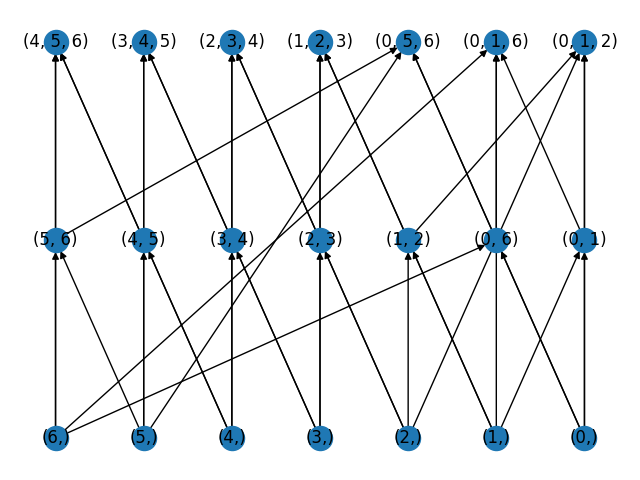
\includegraphics[width=.8\linewidth]{imagenes/7.png}
      \caption{$n = 7$}
    \end{subfigure}%
    \begin{subfigure}{.5\textwidth}
      \centering
      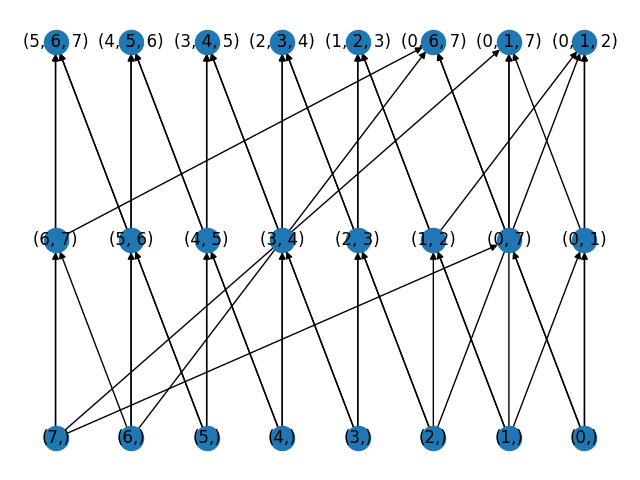
\includegraphics[width=.8\linewidth]{imagenes/8.png}
      \caption{$ n = 8 $}
    \end{subfigure}
    \begin{subfigure}{.5\textwidth}
        \centering
        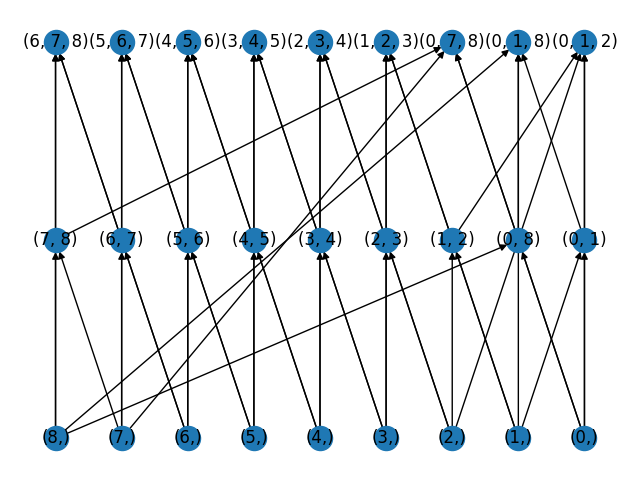
\includegraphics[width=.8\linewidth]{imagenes/9.png}
        \caption{$ n = 9 $}
      \end{subfigure}%
      \begin{subfigure}{.5\textwidth}
        \centering
        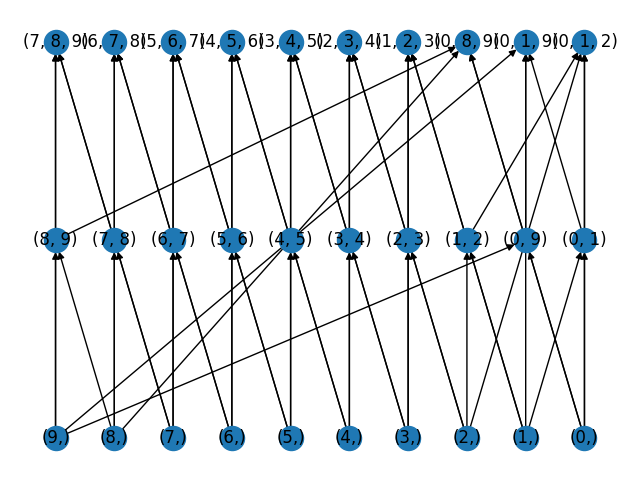
\includegraphics[width=.8\linewidth]{imagenes/10.png}
        \caption{$ n = 10 $}
      \end{subfigure}
\end{figure}
\begin{figure}[h]
     \begin{subfigure}{.5\textwidth}
        \centering
        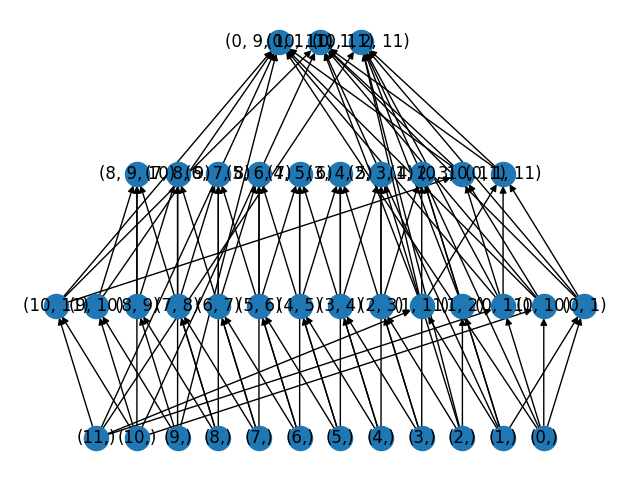
\includegraphics[width=.8\linewidth]{imagenes/11.png}
        \caption{$ n = 11 $}
      \end{subfigure}%
      \begin{subfigure}{.5\textwidth}
        \centering
        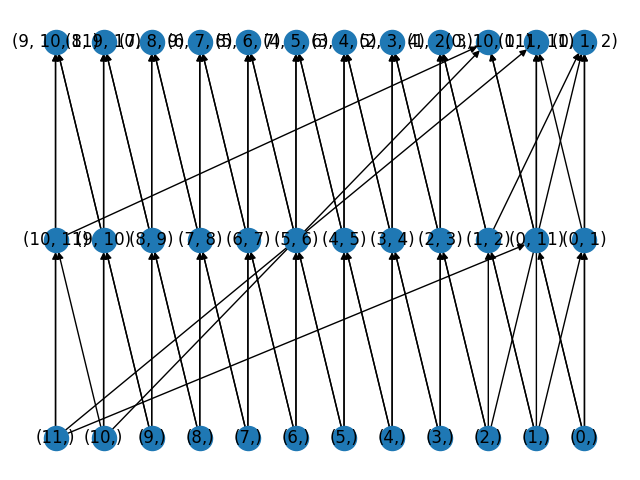
\includegraphics[width=.8\linewidth]{imagenes/12.png}
        \caption{$ n = 12 $}
      \end{subfigure}
\end{figure}
\begin{figure}[h]
      \begin{subfigure}{.5\textwidth}
        \centering
        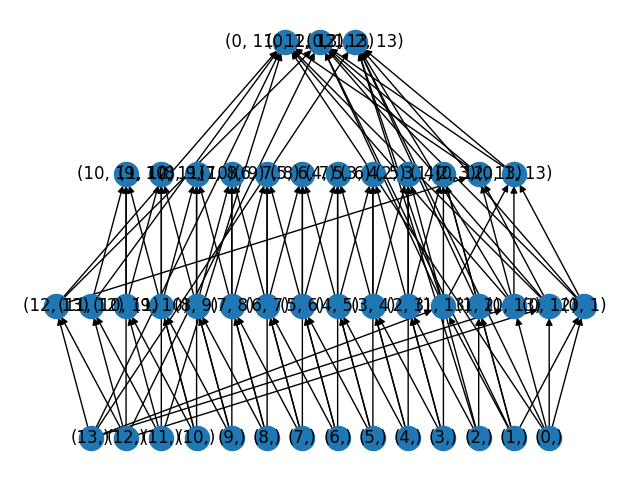
\includegraphics[width=.8\linewidth]{imagenes/13.png}
        \caption{$ n = 13 $}
      \end{subfigure}%
      \begin{subfigure}{.5\textwidth}
        \centering
        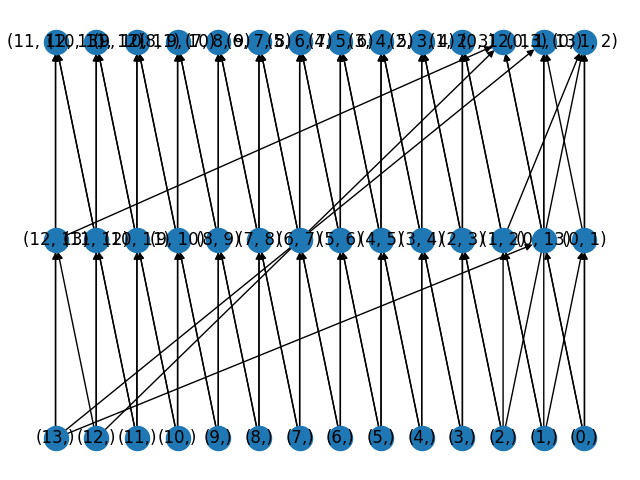
\includegraphics[width=.8\linewidth]{imagenes/14.png}
        \caption{$ n = 14 $}
      \end{subfigure}
    \caption{Distintas fases de la sucesión aproximativa de la circunferencia.}
    \label{circunferencia}
\end{figure}
\newpage
Si avanzamos más en la sucesión, podemos ver cómo se van a\~nadiendo puntos, pero se mantiene un claro patrón:
\begin{figure}[h]
    \begin{subfigure}{.5\textwidth}
      \centering
      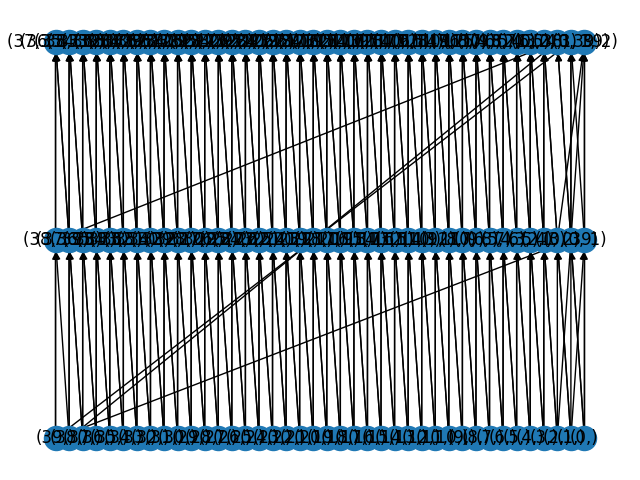
\includegraphics[width=.8\linewidth]{imagenes/40.png}
      \caption{$n = 40$}
    \end{subfigure}%
    \begin{subfigure}{.5\textwidth}
      \centering
      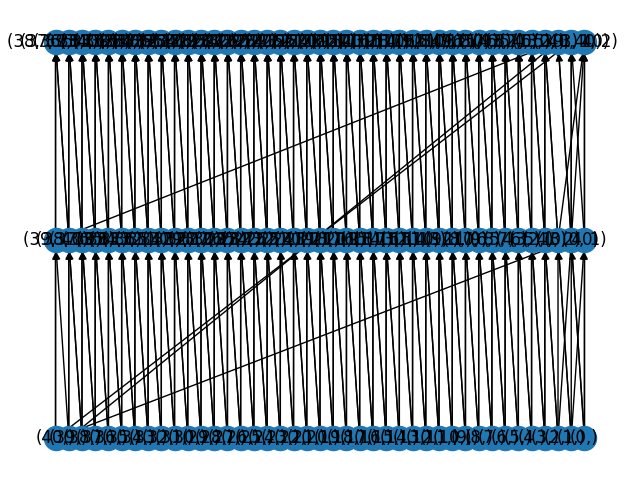
\includegraphics[width=.8\linewidth]{imagenes/41.png}
      \caption{$ n = 41 $}
    \end{subfigure}
    \begin{subfigure}{.5\textwidth}
        \centering
        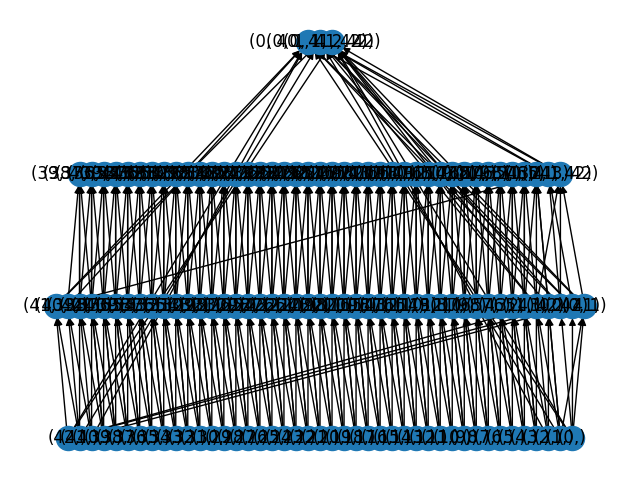
\includegraphics[width=.8\linewidth]{imagenes/42.png}
        \caption{$ n = 42 $}
      \end{subfigure}%
      \begin{subfigure}{.5\textwidth}
        \centering
        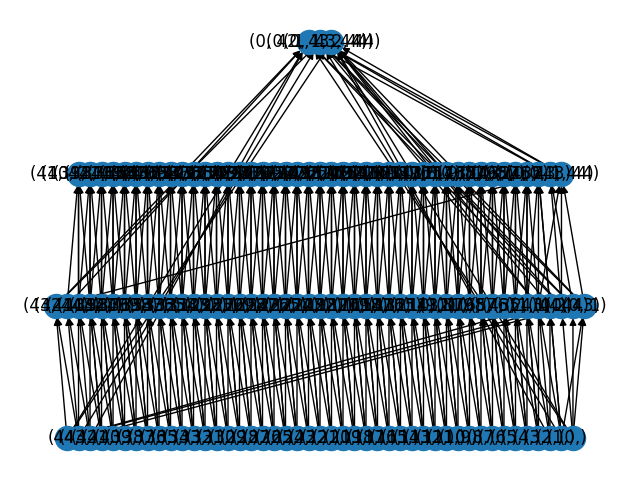
\includegraphics[width=.8\linewidth]{imagenes/44.png}
        \caption{$ n = 44 $}
      \end{subfigure}
\end{figure}

\appendix 
\chapter{Complejos simpliciales}\label{apendice}
En este apéndice vamos a definir brevemente los conceptos relacionados con los complejos simpliciales que aparecen a lo largo del trabajo. 
\begin{definition}
  Un complejo simplicial abstracto $ K $  es una dupla $ (V_K,S_K) $ formada por un conjunto de puntos $ V_K $ a los que llamaremos \textbf{vértices} y un subconjunto $ S_K\subc \pcal(V) $ tal que si $ \sigma\in S_K $, todo $ \tau\subc \sigma $, que llamaremos \textbf{cara} de $ \sigma $, está a su vez en $ S_K $, y además $ \{v\}\in S_K $ para todo $ v\in V_K $. A los elementos de $ S_K $ los llamaremos \textbf{símplices}. Normalmente identificaremos $ K $ con $ S_K $.
\end{definition}
Visto esto, tenemos que estudiar las aplicaciones entre complejos:
\begin{definition}
  Dados dos complejos $ K $ y $ L $, y una aplicación $ \vf:V_K\lra V_L $, decimos que es una \textbf{aplicación simplicial} si para todo $ \sigma \in K $, $ \vf(\sigma)\in L $.
\end{definition}
 
Ahora veamos cómo representarlos en el espacio:
\begin{definition}
  La realización geométrica de un símplice $ \sigma= \{v_0,...,v_n\} $ de un complejo abstracto es el conjunto de combinaciones lineales convexas formales
  \begin{gather*}
    \ol{\sigma } = \left\{\sum_{i=0}^n t_iv_i\mid \sum_{i}t_i = 1, t_i\in [0,1]\right\}.
  \end{gather*}
 Cada s'implice tiene una topolog'ia dada por la m'etrica 
 \begin{gather*}
     \dd(\sum_i t_iv_i ,\sum_i s_iv_i) = \sqrt{\sum_i (t_i-s_i)\sq }
 \end{gather*}
 El \textbf{baricentro} $ b(\sigma) $ de un símplice es el punto resultado de fijar todas las coordenadas $ t_i=\frac{1}{\#\sigma} $.
\end{definition}
\begin{definition}
  La realización geométrica $ \abs{K} $ de un complejo simplicial es la unión de las realizaciones de todos sus símplices con la topología cuyos cerrados son los $ C\subc \abs{K} $ tales que $ C\cap\ol{\sigma } $ es cerrado en $ \ol{\sigma} $ para todo $ \sigma\in K $ (la topolog'ia final con respecto a los $\ol{\sigma}$).
\end{definition}
Si $ K $ es finito, esta coincide con la topología  es la misma que induce la métrica 
\begin{gather*}
  \text{d}(\sum_{v\in K}\alf_v v,\sum_{v\in K}\beta_v v ) = \sqrt[]{\sum_{v\in K}(\alf_v-\beta_v)\sq }.
\end{gather*}

Al espacio m'etrico dado por $(\abs{K},\dd)$ lo denotaremos por $\abs{K}_m$.

\begin{definition}
  Dado un $ x\in \abs{K} $, que podemos representar como $ x = \sum_{v\in K}\alf_v v $ en general, llamamos \textbf{soporte} de $ x $ al símplice $ \{v\mid \alf_v>0\} $ y \textbf{estrella} de un v'ertice $v$ al conjunto $\St(v,\abs{K}) = \{x\in \abs{K}\mid v\in \sop(x)\}$.
\end{definition}

\begin{observation}
  Una aplicación simplicial $ \vf:K\lra L $ induce otra aplicación continua entre las realizaciones geométricas dada por 
  \begin{gather*}
    \begin{matrix}
    \abs{\vf}: \ &\abs{K} &\longrightarrow &\abs{L} \\
    &\sum_{v\in K}\alf_v v &\mapsto &\sum_{v\in K}\alf_v \vf(v).
    \end{matrix}
  \end{gather*}
  Está bien definida porque $\sop(v) $ siempre es un símplice de $ K $, y por tanto $ \vf(\sop(v)) $ lo es de $ L $.
\end{observation}



\begin{definition}\label{subdiv}
  La \textbf{subdivisión baricéntrica} $ K' $ de un complejo $ K $ es el complejo cuyos vértices son los símplices de $ K $ y cuyos símplices son las cadenas de símplices de $ K $. La aplicación lineal dada por
  \begin{gather*}
    \begin{matrix}
    s_K: \ &\abs{K'} &\longrightarrow &\abs{K} \\
    &\sigma  &\mapsto &s_K(\sigma)=b(\sigma) = \sum_{v\in \sigma }\frac{v}{\#\sigma}
    \end{matrix}
  \end{gather*}
  es un homeomorfismo. De hecho, ambas realizaciones se pueden construir de tal forma que sean iguales y $ \abs{s_K }$ sea la identidad.
\end{definition}
\begin{proposition}\label{subdivbar}
  Si escogemos como vértices de la realización de $ K'  $ los baricentros de los símplices de $ K  $, entonces $ \abs{K' } = \abs{K } $ como espacios topológicos y $s_K $ es la identidad.
\end{proposition}
\begin{proof}
  Si realizamos $ K  $ con un conjunto de vértices $ \{v_i\}_{i\in I}  $, cada símplice de $ K'  $ vendrá dado por unos  vértices $ \{b_{\sigma_0 },...,b_{\sigma_m }\} $ donde $ \sigma_0\subset \sigma_1\subset...\subset \sigma_m  $ es una cadena de símplices de $ K  $. Desde luego, todos los vértices de posibles símplices de $ K'  $ son puntos en la realización de un mismo símplice de $ K  $, y por ende toda realización de un símplice de $ K'  $ está contenida en una de un símplice  de $K  $. 
  
  Recíprocamente, queremos ver todo punto $x$ en la realización de un símplice $ \sigma = \{v_0,...,v_m \}\in K  $ está también en la realización de uno de $K'$. Si $ x\in \ol{\sigma } $, pongamos $ x = \sum_{i=0}^m t_iv_i $ y reordenemos y eliminemos vértices de tal forma que  $ t_0\geq t_1\geq...\geq t_m >0 $.  Queremos reescribir $ x  $ como combinación convexa de vértices de $K'$ que formen un símplice, es decir, de baricentros de una cadena de símplices de $K$. Observamos, según la intuición geométrica, que los baricentros que intervengan en la expresión de nuestro punto tendrán que ser los asociados a las caras más próximas al punto, y estas distancias vienen representadas por las coordenadas respecto a los vértices. De esta forma, si denotamos $ \tau_0 = \{v_0\},...,\tau_{m-1} = \{v_0,...,v_{m-1}\},\tau_m = \sigma  $, podemos plantear la ecuación 
  \begin{gather*}
    x = \sum_{i=0}^m t_i v_i = \alf_0 b_{\tau_0}+...+\alf_m b_{\tau_m}.
  \end{gather*}
  Sustituyendo cada baricentro por su valor, llegamos a las ecuaciones 
  \begin{gather*}
    \sum_{i=0}^m t_iv_{i} = \sum_{i=0}^m \left(\frac{\alf_i }{i+1}+...+\frac{\alf_m}{m+1}\right)v_i,
  \end{gather*}
  y reescribiéndolo como sistema, 
  \begin{gather*}
    \left\{ \begin{matrix}
        \alf_0 + & \frac{\alf_1 }{2} +...+&\frac{\alf_m }{m+1} = t_0\\ 
      & \frac{\alf_1 }{2} +...+&\frac{\alf_m }{m+1} = t_1 \\ 
      &&\vdots \\ 
      & & \frac{\alf_m }{m+1} = t_m
    \end{matrix}\right.
  \end{gather*}
  Este sistema tiene solución única y esta es $\alf_i = (t_{i}-t_{i+1})(i+1) \geq 0$. Sumando las ecuaciones del sistema se desprende también que $\sum_i \alf_i = \sum_i t_i =1 $ y podemos escribir $ x  $ como combinación de vértices de $ K'  $, de donde $ \abs{K' } = \abs{K } $ como conjuntos. En cuanto a la topología, si $ C$ es cerrado en $ \ol{\sigma } $, toda $ C\cap \ol{\tau } = C\cap \ol{\sigma }\cap \ol{\tau }$ es cerrada por ser intersección de cerrados, así que todo cerrado de $ \abs{K}  $ lo es de $ \abs{K' } $. Recíprocamente, todo $ \ol{\sigma } \subc \abs{K} $ es unión de una cantidad finita de $ \ol{\tau }\subc \abs{K' } $, y por tanto $ C\cap \ol{\sigma} = \bigcup_\tau C\cap\ol{\tau } $ es cerrada.
\end{proof}
Enunciamos ahora un lema que nos servir'a a para probar la siguiente proposici'on:
\begin{lemma}\label{idhomotopia}
    La identidad $\id : \abs{K}\lra \abs{K}_m$ es una equivalencia homot'opica.
\end{lemma}
\begin{proof}
    La prueba se puede encontrar en \cite[p. 302]{mardešić1982shape}.
\end{proof}

A lo largo de todo el trabajo haremos uso del siguiente criterio para probar que las realizaciones de dos aplicaciones simpliciales son hom'otopas:
\begin{definition}
  Diremos que dos aplicaciones continuas $ g,f: X \lra \abs{K } \ (\abs{K}_m) $ de un espacio topológico en la realización de un complejo simplicial son \textbf{simplicialmente cercanas} si, para todo $ x\in X  $, las imágenes $ f\px $ y $ g\px  $ pertenecen a la realización de un $ \sigma \in K  $.
\end{definition}
\begin{proposition}\label{simplicialmentecercanas}
  Dos aplicaciones simplicialmente cercanas son siempre homótopas.
\end{proposition}
\begin{proof}
  Hagamos primero el caso m'etrico. Por ser simplicialmente cercanas, la aplicaci'on
  \begin{gather*}
    \begin{matrix}
    H: \ &X \times I &\longrightarrow &\abs{K}_m \\
    &(x,t) &\mapsto &tf\px +(1-t)g\px
    \end{matrix}
  \end{gather*}
  está bien definida. La continuidad es sencilla gracias a la m'etrica:
  \begin{gather*}
      \dd(H(x,t),H(x_0,t_0)) = \dd(tf(x)+(1-t)g\px, t_0f(x_0)+(1-t_0)g(x_0)) = \\ 
      \dd(tf(x)+(1-t)g\px,tf(x_0)+(1-t)g(x_0)) +\\ 
      \dd(tf(x_0)+(1-t)g(x_0),t_0f(x_0)+(1-t_0)g(x_0)), 
  \end{gather*}
   donde las distancias anteriores se pueden reducir arbitrariamente por la continuidad de $f$ y $g$. En el caso de estar en la topolog'ia final, el Lema \ref{idhomotopia} y el caso m'etrico nos aseguran la homotop'ia $\id \circ f\simeq \id \circ g$. Si llamamos $j$ a la inversa homot'opica de la identidad, 
   \begin{gather*}
       f\simeq j\circ \id\circ  f\simeq j \circ \id \circ g \simeq g,
   \end{gather*}
   concluyendo la demostraci'on.
\end{proof}


\begin{definition}
  Dadas aplicaciones simpliciales entre complejos  $\vf,\psi :K\lra L$, diremos que son \textbf{contiguas} si para cada $ \sigma\in K $ se tiene $ \vf(\sigma)\cup \psi(\sigma)\in L $.
\end{definition}

\begin{proposition}\label{contiguashomotopas}
  Si dos aplicaciones simpliciales $ \vf  $ y $ \psi  $ son contiguas, sus aplicaciones asociadas entre las realizaciones son homótopas. 
\end{proposition}
\begin{proof}
  Tenemos dos aplicaciones $ \abs{\vf},\abs{\psi}:\abs{K}\lra\abs{L} $ continuas tales que dado $ x\in \abs{K} $, será $ x\in \ol{\sigma } $ para algún $ \sigma\in K $. Entonces $ \abs{\vf(x)}$ y $ \abs{\psi(x)}$ pertenecen a $ \ol{\vf(\sigma)\cup\psi(\sigma ) }$ para todo $ x\in \abs{K}$, es decir, son simplicialmente cercanas y por tanto homótopas.
\end{proof}
\iffalse
\begin{definition}
  Un \textbf{cono simplicial} es un complejo $ K $ que tiene un vértice $ a $ tal que para todo $ \sigma\in K $, $ \sigma\cup \{a\} $ también es símplice de $ K $.
\end{definition}
\begin{proposition}\label{conosimp}
  Si $ K $ es un cono simplicial, $ \abs{K} $ es contráctil.
\end{proposition}
\begin{proof}
  Basta usar la proposición anterior: la identidad es contigua a la aplicación que envía cada vértice a $ a $.
\end{proof}
\fi

\nocite{barmak2011algebraic}
\nocite{Hatcher:478079}
\nocite{jpmayfinitespaces}
\nocite{stong}

\newpage
\printbibliography

\end{document}